%%%%%%%%%%%%%%%%%%%%%%%%%%%%%%%%%%%%%%%%%%%%%%%%%%%%%%%%%%%%%%%%%%%
%%% Documento LaTeX 											%%%
%%%%%%%%%%%%%%%%%%%%%%%%%%%%%%%%%%%%%%%%%%%%%%%%%%%%%%%%%%%%%%%%%%%
% Título:	Entrenamiento cognitivo en realidad virtual
% Autor:  Antonio Jiménez Amador
% Fecha:  2023-09-04
%%%%%%%%%%%%%%%%%%%%%%%%%%%%%%%%%%%%%%%%%%%%%%%%%%%%%%%%%%%%%%%%%%%
%	Modo:					PDFLaTeX.
%%%%%%%%%%%%%%%%%%%%%%%%%%%%%%%%%%%%%%%%%%%%%%%%%%%%%%%%%%%%%%%%%%%







%%%%%%%%%%%%%%%%%%%%%%%%%%%%%%%%%%%%%%%%%%%%%%%%%%%%%%%%%%%%%%%%%%%
%
% IMPORTANTE. PARA MANTENER LA ESTRUCTURA DE CARPETAS DEL PROYECTO
% Configurar TeXstudio -> Órdenes
% PdfLaTex -> pdflatex.exe -synctex=1 -interaction=nonstopmode --output-directory=00.Auxiliar/01.Output --aux-directory=00.Auxiliar/02.Build %.tex
% BibTex -> bibtex.exe 00.Auxiliar/02.Build/% -include-directory=00.Auxiliar/02.Build
%
%%%%%%%%%%%%%%%%%%%%%%%%%%%%%%%%%%%%%%%%%%%%%%%%%%%%%%%%%%%%%%%%%%%



% Preámbulo del documento.
%-----------------------------------------------------------------%
% Clase de documento: libro
\documentclass[12pt,a4paper]{book} % article, report, book.

% Preámbulo: paquetes, comandos, entornos, estilos y título de página.
%4 Estilo y formato%
\usepackage{imakeidx} %MakeIndex%
%Comando para crear glosario (index en inglés)
\makeindex[columns=2, title=Glosario, intoc]
%\usepackage{showidx} % Hace que cada comando \index se imprima en la página donde se ha puesto (útil para corregir los índices)
\usepackage{fancyhdr}	%cabeceras y pies mejor que con \pagestyle{}%
\setlength{\headheight}{16pt}% ...at least 16pt
\usepackage{titlesec,titletoc} %Formateo de secciones y títulos%
\raggedbottom %Para fragmentar versos en varias páginas%
\usepackage{alltt} % Define el environment alltt, como verbatim, excepto que \, { y } tienen su significado normal. Se describe en el fichero alltt.dtx.
\usepackage[pdftex,bookmarksnumbered,hidelinks]{hyperref} %hyper-references%
\usepackage{minitoc} % Para poner tablas de contenido en cada capítulo.
\usepackage{listings} % Para escribir piezas de código C, Python, etc. %
%listings configuration
\lstset{
  language=Python, %Puede ser C, C++, Java, etc.
  showstringspaces=false,
  formfeed=\newpage,
  tabsize=4,
  commentstyle=\itshape,
  basicstyle=\footnotesize\ttfamily,
  escapeinside={(@}{@)},
  morekeywords={models, lambda, forms}
}
\renewcommand{\lstlistingname}{Listado}

\usepackage{tipa} % tipografía IPA (International Phonetic Alphabet)
\usepackage{longtable} %Entorno Longtable, fracciona tablas a lo largo de páginas%
\usepackage{xcolor}
\usepackage{colortbl}
\usepackage{acronym}  %Para expandir automáticamente los acrónimos
\usepackage{emptypage} %Para eliminar el número de página en páginas sin contenido (\cleardoublepage)

\usepackage{graphicx}
\graphicspath{{figuras/}}
\usepackage{datenumber}
\usepackage{multirow}
%\usepackage{babel}

\usepackage{subcaption}
\usepackage[font=scriptsize,labelfont=bf]{caption}

\usepackage{float}

%1 Codificación e idioma%
\usepackage[utf8]{inputenc} %Codificación en latin-1%
\usepackage[T1]{fontenc} %Codificación de fuente%
\usepackage[spanish]{babel}  %Hyphenation (Guionado) en español%
\usepackage{eurosym} %Tipografía euro ()%

%---------------------------------
%\setlength{\marginparwidth}{2cm}
\usepackage{todonotes}
%\usepackage[disable]{todonotes}
%---------------------------------

\input{01.Estructura/01.Configuracion/02.Comandos.tex}
\input{01.Estructura/01.Configuracion/03.Entornos.tex}
\input{01.Estructura/01.Configuracion/04.EstiloPagina.tex}

% Document body.
%-------------------------------------------------------------------%
\begin{document}

% Formato de documento hasta el capítulo 1 (sin incluirlo)
\frontmatter


% ToDo List.
%%%%%%%%%%%%%%%%%%%%%%%%%%%%%%%%%%%%%%%%%%%%%%%%%%%%%%%%%%%%%%%%%%%%
%%% Documento LaTeX 																						%%%
%%%%%%%%%%%%%%%%%%%%%%%%%%%%%%%%%%%%%%%%%%%%%%%%%%%%%%%%%%%%%%%%%%%
% Título:	Lista de acrónimos
% Autor:  Ignacio Moreno Doblas
% Fecha:  2014-02-01, actualizado 2019-11-11
%%%%%%%%%%%%%%%%%%%%%%%%%%%%%%%%%%%%%%%%%%%%%%%%%%%%%%%%%%%%%%%%%%%
% !TEX root = A0.TFG.tex

%Lista de acrónimos
%\chapterbeginx{Cosas por hacer}

\listoftodos

%\chapterend


% Los tres ficheros siguientes simulan el formato de las páginas
% iniciales que también puedes descargar en word de la web de la ETSITT.
%
% Portada.
%%% Tipos de portada %%%
%	1. \maketitle
%	2. titlepage
%%%%%%%%%%%%%%%%%%%%%%%%

%	1. \maketitle
%%%%%%%%%%%%%%%%%%%%%%%%
%\maketitle
\thispagestyle{empty}

%	2. titlepage
%%%%%%%%%%%%%%%%%%%%%%%%
\begin{titlepage}
 
 
\newlength{\centeroffset}
\setlength{\centeroffset}{-0.5\oddsidemargin}
\addtolength{\centeroffset}{0.5\evensidemargin}
\thispagestyle{empty}

\noindent\hspace*{\centeroffset}\begin{minipage}{\textwidth}

\centering
\includegraphics[width=0.8\textwidth]{01.Estructura/02.Portada/00.Figuras/01.logo_ugr.jpg}\\[1.4cm]

\textsc{ \Large TRABAJO FIN DE GRADO\\[0.2cm]}
\textsc{ INGENIERÍA INFORMÁTICA}\\[1cm]
% Upper part of the page
% 
% Title
{\Large\bfseries \tfgtitlename\\
}
\noindent\rule[-1ex]{\textwidth}{3pt}\\[3.5ex]
{\large\bfseries \tfgsubtitlename}
\end{minipage}

\vspace{0.5cm}
\noindent\hspace*{\centeroffset}\begin{minipage}{\textwidth}
\centering



\textbf{Autor}\\ \tfgauthorname \\[2.5ex]
\textbf{Directores}\\
{\tfgtutornameA\\
\tfgtutornameB}\\[1cm]
\includegraphics[width=0.3\textwidth]{01.Estructura/02.Portada/00.Figuras/02.etsiit_logo.png}\\[0.1cm]
\textsc{Escuela Técnica Superior de Ingenierías Informática y de Telecomunicación}\\
\textsc{---}\\
Granada, \tfgmes{} de \tfganno
\end{minipage}

%\addtolength{\textwidth}{\centeroffset}
%\vspace{\stretch{2}}
\end{titlepage}








% Resumen del TFG en español
%%%%%%%%%%%%%%%%%%%%%%%%%%%%%%%%%%
% Página de resumen del proyecto %
%%%%%%%%%%%%%%%%%%%%%%%%%%%%%%%%%%
% !TEX root = A0.TFG.tex

\pagestyle{fancy}
\renewcommand{\headrulewidth}{0pt}
\addstarredchapter{Resumen}

\begin{center}
	\scshape
	E.T.S. de Ingenierías Informática y de Telecomunicación, Universidad de Granada
\end{center}

\bigskip

\begin{center}
	\Large \scshape
	\textbf{\tfgtitlename}
\end{center}

\bigskip \bigskip \bigskip

\begin{minipage}{\textwidth}

\textbf{Autor:} \tfgauthorname

\medskip

\textbf{Tutores:} \tfgtutornameA , \tfgtutornameB

\medskip

%\textbf{Cotutor:} <Nombre del cotutor>\ (elimina esta línea si no hay cotutor)

\medskip

\textbf{Departamento:} Lenguajes y Sistemas Informáticos

\medskip

\textbf{Titulación:} Grado en Ingeniería Informática

\medskip

\textbf{Palabras clave:} Realidad virtual, entrenamiento cognitivo, deterioro cognitivo, mayores, videojuegos, juego serio, Unity, Oculus.

\bigskip \bigskip


\end{minipage}

\begin{center}
	\textbf{Resumen}
\end{center}


\todo[inline, size=\tiny]{Resumen español}

El resumen debe ser una breve descripción del contexto del proyecto,
sus objetivos y los resultados obtenidos. Se recomienda que no exceda
esta página.


\blankpage


% Resumen del TFG en inglés
%%%%%%%%%%%%%%%%%%%%%%%%%%%%%%%%%%%%%%%%%%%
% Página de resumen del proyecto en inglés%
%%%%%%%%%%%%%%%%%%%%%%%%%%%%%%%%%%%%%%%%%%%
% !TEX root = A0.TFG.tex

\pagestyle{fancy}
\addstarredchapter{Abstract}

\begin{center}
	\scshape
	E.T.S. de Ingenierías Informática y de Telecomunicación, Universidad de Granada
\end{center}

\bigskip

\begin{center}
	\Large \scshape
	\textbf{\tfgtitlenameENG}
\end{center}

\bigskip \bigskip \bigskip

\begin{minipage}{\textwidth}

\textbf{Author:} \tfgauthorname

\medskip

\textbf{Supervisors:} \tfgtutornameA , \tfgtutornameB

\medskip

%\textbf{Co-supervisor:} <Nombre del cotutor>\ (elimina esta línea si no hay cotutor)

\medskip

\textbf{Department:} <Department name>

\medskip

\textbf{Degree:} Grado en Ingeniería de <nombre de la titulación>

\medskip

\textbf{Keywords:} Keywords (separated by commas) describing and characterizing the topic of the work.

\bigskip \bigskip


\end{minipage}

\begin{center}
	\textbf{Abstract}
\end{center}

The abstract should briefly describe the project context, goals and
obtained results. It should not exceed this page.

\blankpage


% Autorización alumno.
\chapter*{}
\thispagestyle{empty}

\noindent\rule[-1ex]{\textwidth}{2pt}\\[4.5ex]

Yo, \textbf{\tfgauthorname}, alumno de la titulación Ingeniería Informática de la \textbf{Escuela Técnica Superior
de Ingenierías Informática y de Telecomunicación de la Universidad de Granada}, con DNI 75574393G, autorizo la
ubicación de la siguiente copia de mi Trabajo Fin de Grado en la biblioteca del centro para que pueda ser
consultada por las personas que lo deseen.

\vspace{6cm}

\noindent Fdo: \tfgauthorname

\vspace{2cm}

\begin{flushright}
Granada a  de \tfgmes{} de \tfganno .
\end{flushright}


% Autorización tutores.
\chapter*{}
\thispagestyle{empty}

\noindent\rule[-1ex]{\textwidth}{2pt}\\[4.5ex]

D. \textbf{\tfgtutornameA}, profesor del Departamento de Lenguajes y Sistemas Informáticos de la Universidad de Granada.

\vspace{0.5cm}

Dña. \textbf{\tfgtutornameB}, profesora del Departamento de Lenguajes y Sistemas Informáticos de la Universidad de Granada.


\vspace{0.5cm}

\textbf{Informan:}

\vspace{0.5cm}

Que el presente trabajo, titulado \textit{\textbf{\tfgtitlename, \tfgsubtitlename}},
ha sido realizado bajo su supervisión por \textbf{\tfgauthorname}, y autorizamos la defensa de dicho trabajo ante el tribunal
que corresponda.

\vspace{0.5cm}

Y para que conste, expiden y firman el presente informe en Granada a 1 de \tfgmes{} de \tfganno.


\vspace{0.5cm}

\textbf{Los directores:}

\vspace{4cm}

\noindent \textbf{\tfgtutornameA \ \ \ \ \ \tfgtutornameB}

% Los dos siguientes archivos son opcionales
% Coméntalos si no los quieres usar

% Dedicatoria.

\cleardoublepage
\thispagestyle{empty} % No queremos mostrar ningún encabezamiento ni pie de página.

\begin{minipage}[c][\textheight][c]{\textwidth} %[pos][height][inner-pos]{width}
\raggedleft %\flushleft


A mi familia. \\
Por apoyarme durante\\
este largo camino.

\bigskip

\emph{\tfgauthorname}

\end{minipage}

\blankpage


% Agradecimientos.
%%%%%%%%%%%%%%%%%%%%%%%%%%%%%%%%%%%
% Página de resumen del proyecto %
%%%%%%%%%%%%%%%%%%%%%%%%%%%%%%%%%%
% !TEX root = A0.TFG.tex

\pagestyle{fancy}
%\renewcommand{\headrulewidth}{0pt}


\chapterbeginx{Agradecimientos}

\todo[inline, size=\tiny]{Agradecimientos}

Este apartado es opcional. En él se incluirían los agradecimientos personales y profesionales. Si no los hubiere, debe eliminarse esta página y la siguiente (para ello puedes comentar la línea 58 de A0.TFG.tex).

\chapterend


\blankpage


% Acrónimos
%%%%%%%%%%%%%%%%%%%%%%%%%%%%%%%%%%%%%%%%%%%%%%%%%%%%%%%%%%%%%%%%%%%
%%% Documento LaTeX 																						%%%
%%%%%%%%%%%%%%%%%%%%%%%%%%%%%%%%%%%%%%%%%%%%%%%%%%%%%%%%%%%%%%%%%%%
% Título:	Lista de acrónimos
% Autor:  Ignacio Moreno Doblas
% Fecha:  2014-02-01, actualizado 2019-11-11
%%%%%%%%%%%%%%%%%%%%%%%%%%%%%%%%%%%%%%%%%%%%%%%%%%%%%%%%%%%%%%%%%%%
% !TEX root = A0.TFG.tex

%Lista de acrónimos
\chapterbeginx{Acrónimos}

\begin{acronym}[DLMS/COSEMM]
%Añade los acrónimos por orden alfabético

	\acro{ETSITT}{Escuela Técnica Superior de Ingenierías Informática y de Telecomunicación}
	\acro{GDD}{Game Design Document}
	\acro{HMD}{Head Mounted Display}
	\acro{JSON}{JavaScript Object Notation}
	\acro{RV}{Realidad Virtual}
	\acro{TFG}{Trabajo Fin de Grado}
	\acro{UGR}{Universidad de Granada}
	\acro{VRTK}{Virtual Reality Toolkit}
	
\end{acronym}

\chapterend


% Tabla de contenidos, figuras y tablas.
\input{01.Estructura/06.Contenido/02.TablaContenidos.tex}
\input{01.Estructura/06.Contenido/03.TablaFiguras.tex}
\input{01.Estructura/06.Contenido/04.TablaTablas.tex}

% Formato de documento durante los capítulos.
\mainmatter

% Prólogo. Opcional
%\input{01.Estructura/07.Prologo/01.Prologo.tex}

% Parte I. Introducción
\part{Introducción}

% Capítulo 01. Introducción y objetivo
%%%%%%%%%%%%%%%%%%%%%%%%%%%%%%%%%%%%%%%%%%%%%%%%%%%%%%%%%%%%%%%%%%%
%%% Documento LaTeX 																						%%%
%%%%%%%%%%%%%%%%%%%%%%%%%%%%%%%%%%%%%%%%%%%%%%%%%%%%%%%%%%%%%%%%%%%
% Título:		Introducción
% Autor:  	Ignacio Moreno Doblas
% Fecha:  	2014-02-01, actualizado 2019-11-11
% Versión:	0.5.0
%%%%%%%%%%%%%%%%%%%%%%%%%%%%%%%%%%%%%%%%%%%%%%%%%%%%%%%%%%%%%%%%%%%
% !TEX root = A0.TFG.tex

\chapterbegin{Introducción}
\label{chp:Introduccion}

\section{Introducción}


El ser humano está en constante desarrollo desde que nace. Este proceso no es únicamente físico y biológico, si no que da forma a cada persona desde temprana edad mediante cambios psicológicos y cognitivos. La cognición es la capacidad de percibir información del entorno para posteriormente procesarla y obtener conocimientos y valoraciones. Esto engloba procesos cognitivos como el razonamiento, la memoria, la atención, la capacidad de resolución de problemas y los sentimientos.

 Durante la vida de una persona, la cognición se desarrolla rápidamente durante sus primeros años de vida y, en condiciones normales, se mantiene estable durante la vida adulta. Ciertos motivos externos pueden causar un deterioro anormal de las capacidades cognitivas de un individuo, como son por ejemplo algunas enfermedades neurodegenerativas como el Alzheimer u otros tipos de demencia. Incluso en personas sanas, existe un deterioro natural de las habilidades cognitivas que va ligado a la edad, por lo que es común que las personas de la tercera edad sufran de problemas cognitivos como pérdidas de memoria, dificultades de comunicación o faltas de atención. Estos son problemas que las personas mayores sufren en su día a día y que en ocasiones no les permite disfrutar plenamente de su vida y ocio diario.
 
Afortunadamente, la cognición es una característica humana y como muchas otras, puede ser entrenada, reforzada e incluso recuperada después de verse deteriorada. Para esto existen los llamados entrenamientos cognitivos, que suelen venir asociados a ejercicios mentales. Cualquier persona puede realizar estos ejercicios y ver reforzadas sus capacidades cognitivas, pero son especialmente útiles para prevenir un deterioro anticipado de la cognición en personas mayores y como método de rehabilitación para personas que a causa de alguna enfermedad han visto sus capacidades cognitivas dañadas.

Estos entrenamientos existen desde hace décadas, pero han ido evolucionando con el avance de las nuevas tecnologías. Ahora en vez de tratarse de ejercicios en papel que deben realizarse de manera supervisada, se puede acceder a ellos mediante aplicaciones móviles o páginas web, que permiten un uso más cómodo y atractivo.

Sin embargo, esto tiene un problema asociado: y es que, aunque los ejercicios hayan evolucionado con la tecnología, los principales usuarios de estos ejercicios cognitivos son personas mayores que suelen no estar familiarizados en absoluto con dichas tecnologías. Por tanto, esto genera una barrera adicional para su uso ya que la mayoría de las personas mayores no sabe cómo utilizar estas aplicaciones o páginas web.

Para solventar este problema es necesario facilitar al máximo su uso para los mayores, pero es aún más importante, si cabe, que las personas estén motivadas a realizar los ejercicios. Una falta de motivación puede llegar a reducir en gran medida la efectividad de los entrenamientos cognitivos. 



\section{Motivación}

Hoy en día existen tecnologías como la realidad virtual o RV, que mediante el uso de un visor especial permiten sumergir al usuario en un mundo virtual con un grado de inmersión que ninguna otra tecnología puede alcanzar. Incluso para personas jóvenes y con experiencia tecnológica, la realidad virtual provoca sensaciones extraordinarias y permite vivir experiencias imposibles en la vida real. La RV es una herramienta que usada de forma adecuada puede incrementar de manera considerable la motivación de una persona, especialmente una persona mayor, ya que le abre las puertas a un mundo virtual con el que nunca ha tenido contacto, y el factor sorpresa puede motivarlo a continuar avanzando y descubriendo cosas nuevas.

Es por este motivo, que este proyecto trata de demostrar un posible uso de la realidad virtual aplicada a la realización de ejercicios cognitivos enfocados a personas mayores. Se busca resolver los dos problemas planteados: la falta de motivación y la desconexión tecnológica de las personas mayores.


\section{Objetivo}

El objetivo principal de este proyecto es crear un prototipo de un videojuego que pueda utilizarse para comprobar la efectividad del uso de la realidad virtual como herramienta para el entrenamiento cognitivo en personas mayores.

Para alcanzar este objetivo se va a desarrollar un juego serio\footnote{Juego que tiene un propósito principal no recreativo.}, dentro del cual se presentarán al jugador distintos ejercicios cognitivos basados en ejercicios ya existentes y adaptados al uso de la RV.


\subsection{Objetivos específicos}

Para considerar cumplido el objetivo principal de este proyecto, es necesario cumplir a su vez varios subobjetivos que permitirán el desarrollo del videojuego de forma exitosa:


\begin{itemize}
	\item{Creación de un entorno de realidad virtual especialmente diseñado para ser utilizado por personas mayores.}

	\item{Evaluación de dicho entorno para comprobar que una persona mayor y sin conocimientos tecnológicos sea capaz de interactuar con él de manera cómoda.}

	\item{Diseñar ejercicios de entrenamiento cognitivos adaptados a la realidad virtual a partir de ejercicios tradicionales, manteniendo su funcionamiento central inalterado, asegurando que son efectivos.}

	\item{Diseñar ejercicios cognitivos completamente nuevos, dando pleno uso a las capacidades de la RV de las que carecen los métodos tradicionales.}

	\item{Obtener un videojuego final que sea atractivo y motivador para las personas mayores.}

	\item{El videojuego podrá ser usado de forma personal, o como herramienta guiada por profesionales.}

	\item{Reducir al mínimo las dificultades e inconvenientes que conlleva la RV, especialmente a nivel físico: incomodidades con el casco, posibles cables que limiten el movimiento del usuario, etc.}


\end{itemize}


\section{Estructura de la memoria}

En primer lugar, se va a estudiar la cognición humana y cómo esta puede ser entrenada y desarrollada. Para ello se utilizan diferentes tipos de ejercicios cognitivos, que han ido cambiando con la evolución de las tecnologías. 

Este proyecto busca desarrollar un videojuego de realidad virtual para continuar adaptando estos ejercicios a nuevas tecnologías. Por ello se va a hablar sobre la realidad virtual, su historia y la importancia que tiene hoy en día. Posteriormente se estudiarán cuatro motores de videojuegos, que son los conjuntos de software y tecnologías utilizadas para la creación de videojuegos.

Una vez estudiados estos conceptos fundamentales para el proyecto, se detallará el conjunto de herramientas software y hardware que serán utilizadas para el desarrollo del videojuego, así como la metodología que se seguirá durante el progreso de este TFG.

A continuación, se presenta un diario de desarrollo del videojuego en el que se cuenta paso a paso, y con el apoyo de figuras, todo lo relacionado al diseño y creación del videojuego para la consecución del objetivo del proyecto. Finalmente se cierra esta memoria con unas conclusiones, pensamientos finales y posibles líneas futuras que puede seguir el proyecto.





\chapterend


\part{Estudio del problema}

% Estado del arte.
%%%%%%%%%%%%%%%%%%%%%%%%%%%%%%%%%%%%%%%%%%%%%%%%%%%%%%%%%%%%%%%%%%%
%%% Documento LaTeX 																						%%%
%%%%%%%%%%%%%%%%%%%%%%%%%%%%%%%%%%%%%%%%%%%%%%%%%%%%%%%%%%%%%%%%%%%
% Título:		Introducción
% Autor:  	Ignacio Moreno Doblas
% Fecha:  	2014-02-01, actualizado 2019-11-11
% Versión:	0.5.0
%%%%%%%%%%%%%%%%%%%%%%%%%%%%%%%%%%%%%%%%%%%%%%%%%%%%%%%%%%%%%%%%%%%
% !TEX root = A0.TFG.tex

\chapterbegin{Estado del arte}
\minitoc

\todo[inline, size=\tiny]{Citar las referencias en la bibliografía de las que he obtenido la información del estado del arte}

\section{Cognición}
\label{sec:estadoArte:cognicion}

Uno de los factores que separa a los seres humanos del resto de animales es su mayor desarrollo cognitivo. La cognición es la capacidad para captar, asimilar, procesar y utilizar información obtenida del entorno. Bajo este nombre se incluyen diversos procesos cognitivos como: el aprendizaje, la memoria, la toma de decisiones, la comprensión y el razonamiento.

Los primeros estudios sobre la cognición, desarrollados por Aristóteles, datan del siglo IV A.C. Aristóteles estudió el funcionamiento interno de la mente humana centrándose en la memoria y la percepción. Siempre trató de basar sus estudios en técnicas puramente empíricas mediante la experimentación y la observación. \cite{EA_cog_aristoteles}

No fue hasta el siglo XV durante la Ilustración, que se retomaron los estudios sobre la mente y su funcionamiento. Y más significativamente, durante los siglos XIX y XX.

Durante la segunda mitad del siglo XIX, el auge y desarrollo de la psicología y especialmente de la psicología experimental, impulsó la investigación en el campo cognitivo. El filósofo y psicólogo alemán Wilhelm Wundt (1832-1920) desarrolló el concepto de introspección, una técnica consistente en el autoanálisis de los sentimientos de la persona, exponiéndolos de la forma más objetiva posible. \cite{EA_cog_wundt} La introspección sentó las bases para el desarrollo de las técnicas posteriores, aunque debido a ser puramente subjetiva los psicólogos posteriores intentarán no depender de ella.

Hermann Ebbinghaus (1850-1909), otro psicólogo alemán, dedicó su carrera a la investigación de la memoria. Desarrolló un experimento con el que probar la capacidad de aprendizaje de nueva información, así como la pérdida de ella mediante el olvido. Debido a que el experimento debía evitar la intervención de cualquier conocimiento previo, Ebbinghaus creó hasta 2300 sílabas inexistentes y sin sentido para evitar ser asociadas con palabras reales. La prueba consistía en memorizar en orden aleatorio la mayor cantidad de dichas sílabas y recitarlas posteriormente. El experimento concluyó que el cerebro humano siempre intenta relacionar la nueva información con algún conocimiento anterior, y cuanto mayor es la relación encontrada mejor es la retención en la memoria de la nueva información. \cite{EA_cog_ebbinghaus}

Los estudios de Ebbinghaus le permitieron definir el efecto de posición serial (figura \ref{fig:EA_posicionSerial}): a la hora de memorizar y recitar una lista de elementos, la posición en la lista que ocupan los elementos tiene efecto en la capacidad para memorizarlos. El cerebro humano es capaz de retener mejor la información al principio de una lista (efecto de primacía) así como al final de esta (efecto de recencia), sin embargo, los elementos centrales son que mayor esfuerzo requieren para ser memorizados.



\begin{figure}
  \centering
\includegraphics[width=0.5\textwidth]{03.EstudioProblema/01.EstadoArte/00.Figuras/01.efecto_serial.jpg}
    \caption{Gráfica que representa la curva creada por el efecto se posición serial. \cite{EA_img_efectoPosicionSerial}}
    \label{fig:EA_posicionSerial}
\end{figure}


La cognición y las habilidades y procesos cognitivos van evolucionando a lo largo de la vida de las personas.

Jean Piaget fue un psicólogo suizo que investigó el desarrollo cognitivo en el ser humano durante los primeros años de vida. Tras sus investigaciones concluyó que el desarrollo de los procesos cognitivos puede ser clasificado por etapas de crecimiento: \cite{EA_cog_piaget}

\begin{itemize}
	\item{Etapa sensomotora (0-2 años): Existe inteligencia, pero el conocimiento se basa únicamente en las experiencias. Se desarrollan las capacidades básicas de habla y de comprensión del espacio y el tiempo.}

	\item{Etapa preoperacional (2-7 años): Se desarrolla la memoria y la imaginación. Predomina la resolución intuitiva de problemas y el pensamiento egocéntrico.}

	\item{Etapa operacional concreta (7-12 años): El pensamiento deja de ser egocéntrico y pasa a ser más sistemático y lógico. Se entienden conceptos complejos espaciales y la persona puede utilizar un proceso de pensamiento reversible.}

	\item{Etapa operacional formal (+12 años): La capacidad de pensamiento se vuelve mucho más flexible, con la posibilidad de comprender conceptos abstractos y formular hipótesis para resolver problemas complejos.}

\end{itemize}

Durante la vida de una persona estas capacidades cognitivas adquiridas durante la infancia pueden resultar dañadas, degradadas o incluso perdidas completamente, dificultando o impidiendo a la persona realizar procesos como la toma de decisiones, aprendizaje o la evaluación crítica, así como llevando a la pérdida de memoria, capacidad de expresión o velocidad de procesado de información. \cite{EA_cog_deterioro}

La pérdida de estas capacidades puede estar causada o ser la causa de alguna enfermedad, por ejemplo: el deterioro cognitivo leve, en la que el paciente no puede llevar a cabo algunos procesos cognitivos de la forma esperada pero no afecta en gran medida a su vida diaria.

Trastornos más graves como la enfermedad de Alzheimer pueden llevar a peores consecuencias como la pérdida completa de la memoria inmediata, degradación en las capacidades cognitivas superiores y dificultad en la comunicación movimiento y resolución de problemas abstractos sencillos. \cite{EA_cog_alzheimer}

Incluso en personas sanas, las capacidades cognitivas van disminuyendo con el tiempo, especialmente durante la vejez. Esta degradación es esperada y no conlleva grandes problemas a la vida diaria de las personas. Para frenar y limitar lo máximo posible está degeneración es imprescindible mantener un alto nivel de actividad cognitiva. Este es el objetivo del entrenamiento cognitivo.




\section{Entrenamiento cognitivo}

El entrenamiento cognitivo, también llamado brain training, engloba al conjunto de actividades diseñadas para mantener o mejorar las capacidades cognitivas propias de una persona.

Estas actividades se basan en la neuroplasticidad humana, que significa que el cerebro es capaz de desarrollarse y transformarse en base a las experiencias vividas. Esto implica que el cerebro puede ser entrenado para fomentar el desarrollo de ciertas áreas de este involucradas con los procesos cognitivos. \cite{EA_ent_plasticidad}

Las áreas objetivo de entrenamientos más usuales son aquellas con mayor relación con actividades diarias y por tanto pueden conllevar una mejora notable de las habilidades. La capacidad de memorizar, mantener la atención y la resolución de problemas son los principales procesos que entrenar.

El entrenamiento cognitivo se centra en grupos de personas con carencias cognitivas como aquellas con enfermedades neurodegenerativas como la demencia o el Alzheimer. Aunque todas las personas pueden beneficiarse del entrenamiento, especialmente personas de edad avanzada que con el paso de los años han visto mermadas sus capacidades habituales en memorización, velocidad de procesamiento, razonamiento o psicomotricidad.

El resultado del brain training puede ser muy diverso entre las personas debido a que cada una tiene un rendimiento máximo en cada habilidad. Una vez que el individuo alcanza su estado óptimo en dicha habilidad, le supondrá un esfuerzo mucho mayor continuar mejorando.

Además, hay que tener en cuenta que incluso cuando el entrenamiento mejora las capacidades cognitivas básicas, estas mejoras pueden no trasladarse a acciones más complejas, a pesar de que dichas acciones sean combinaciones de habilidades sencillas.

A día de hoy, la verdadera efectividad del entrenamiento cognitivo está en duda. Los estudios más recientes demuestran que los grandes efectos de antienvejecimiento y prevención de la enfermedad de Alzheimer son falsos y exagerados por las técnicas de marketing. Si bien el entrenamiento tiene un efecto positivo en las habilidades cognitivas, existen otros factores con mayor importancia, como la genética de cada persona. \cite{EA_ent_efectividad}


\section{Ejercicios de Brain Training}
\label{sec:estadoArte:ejerciciosBrainTraining}

Los ejercicios de entrenamiento cognitivo se pueden presentar en multitud de formatos, comenzando por el formato físico en papel. Los cuadernos de ejercicios han sido el medio clásico de realizar entrenamientos cognitivos. Permiten la estimulación mediante el uso de una herramienta conocida, como es el lápiz y papel, a la vez que presenta ejercicios muy variados: memoria, razonamiento, resolución de problemas o comprensión lectora, adaptados a cualquier nivel, desde niños pequeños hasta personas mayores o enfermos. Su sencillez permite que sean fáciles de diseñar, fabricar y distribuir.

\subsection{Cuadernos de ejercicios}

Los cuadernos de estimulación cognitiva de Esteve (figura \ref{fig:EA_cuadernoEsteve}) y Rubio (figura \ref{fig:EA_cuardernoRubio}) son las más populares en España, están enfocados a personas con algún tipo de deterioro cognitivo (leve, moderado o grave) y su estructura de niveles permite una fácil clasificación y progreso en los ejercicios. \cite{EA_ent_esteve}






\begin{figure}[H]
\centering
\begin{minipage}{.5\textwidth}
  \centering
  \includegraphics[width=.7\linewidth]{03.EstudioProblema/01.EstadoArte/00.Figuras/02.cuaderno_esteve.png}
  \captionof{figure}{Cuaderno Esteve. \cite{EA_img_cuadernoEsteve}}
  \label{fig:EA_cuadernoEsteve}
\end{minipage}%
\begin{minipage}{.5\textwidth}
  \centering
  \includegraphics[width=.9\linewidth]{03.EstudioProblema/01.EstadoArte/00.Figuras/03.cuaderno_rubio.jpg}
  \captionof{figure}{Cuaderno Rubio. \cite{EA_img_cuardernoRubio}}
  \label{fig:EA_cuardernoRubio}
\end{minipage}
\end{figure}



\subsection{Juegos grupales}

En ocasiones donde varias personas que vayan a realizar un entrenamiento cognitivo se encuentren juntas, como residencias o centros de día para mayores, se pueden realizar juegos grupales. Estos juegos permiten no solo la mejora de las capacidades cognitivas por los ejercicios si no que también impulsan las relaciones interpersonales y fomentan la creación de un ambiente amigable y alegre durante la sesión de entrenamiento. \cite{EA_ent_grupos}

Estos juegos están diseñados para ser llevados a cabo en grupos: ya sea de forma simétrica, donde cada participante tiene un rol idéntico, o no, en los que una o varias personas ocupan un papel principal en la acción y el resto los complementa con diferentes acciones.

Existen multitud de juegos de este tipo, algunos de ellos son:

\begin{itemize}
	\item{Juego del abanico: Una persona toma el papel principal y debe transmitir al resto una emoción que elija mediante el uso únicamente de movimientos del abanico.}

	\item{Juego de expresiones: Una persona intenta expresar un sentimiento con expresiones faciales y el resto tendrá que adivinarlo.}

	\item{Juego de los nombres: Todos los participantes forman un círculo y por orden deberán decir su nombre y pasar una pelota al siguiente participante. Tras una vuelta completa, cada persona tendrá que decir algo que le guste y lanzar la pelota a cualquier participante diciendo su nombre. Véase figura \ref{fig:EA_juegosAncianos}}

\end{itemize}


\begin{figure}
  \centering
\includegraphics[width=0.8\textwidth]{03.EstudioProblema/01.EstadoArte/00.Figuras/04.juegos_ancianos.jpg}
    \caption{Juego de grupo con pelota. \cite{EA_img_juegoGrupoPelota}}
    \label{fig:EA_juegosAncianos}
\end{figure}

\subsection{Juegos y plataformas online}

Con la proliferación de las nuevas tecnologías en la vida diaria de las personas, los ejercicios de estimulación se han adaptado para sacar todo el provecho que estas tecnologías ofrecen. Los ejercicios clásicos en papel que ofrecen los cuadernos son fácilmente adaptables a un entorno digital mediante el uso de aplicaciones, juegos y páginas web, que son presentados al usuario a través de un ordenador o de un dispositivo móvil como una Tablet.

Este formato es capaz de enriquecer los ejercicios ya que añade la posibilidad de personalizar cada ejercicio para el nivel y las características del usuario, así como usar animaciones, sonidos y nuevos métodos de interacción: pantalla táctil, movimiento del propio dispositivo, reconocimiento de voz, etc.

Estas plataformas online permiten un monitoreo constante de un profesional sin necesidad de estar físicamente presente con el paciente lo que puede aumentar su utilidad y eficacia frente a los cuadernos tradicionales.

\subsubsection{Lumosity}

Lumosity es una aplicación que reúne una serie de juegos muy llamativos para entrenar la mente de manera amena y dinámica. Se categorizan según la habilidad cognitiva que tratan: velocidad de procesamiento, memoria, atención, flexibilidad mental y resolución de problemas. En la figura \ref{fig:EA_lumosity} se pueden ver varios de estas categorías y sus juegos. \cite{EA_ent_lumosity}

\begin{figure}
  \centering
\includegraphics[width=0.5\textwidth]{03.EstudioProblema/01.EstadoArte/00.Figuras/05.lumosity.png}
    \caption{Algunos de los juegos disponibles en Lumosity.}
    \label{fig:EA_lumosity}
\end{figure}


\subsubsection{NeuronUp}

NeuronUp es una plataforma multidispositivo (figura \ref{fig:EA_neuronUp}) enfocada al uso de profesionales para monitorizar los entrenamientos de sus pacientes. Los juegos son más simples que los de Lumosity, pero ofrece una conexión directa y constante con los profesionales, que es importante para llevar un correcto entrenamiento. \cite{EA_ent_neuronup}

\begin{figure}
  \centering
\includegraphics[width=0.5\textwidth]{03.EstudioProblema/01.EstadoArte/00.Figuras/06.neuronup.jpg}
    \caption{Demostración de NeuronUp multidispositivo. \cite{EA_img_neuronup}}
    \label{fig:EA_neuronUp}
\end{figure}


\subsubsection{Brain training RV}

En los últimos años se ha producido un gran auge de la realidad virtual, llegando a estar al alcance de cualquier persona con un teléfono inteligente. Los juegos de entrenamiento cognitivo han aprovechado este entorno virtual para mejorar la inmersión y realismo de sus ejercicios. Actualmente la RV está evolucionando día a día, y los juegos brain training asociados a ella también.

La RV puede usarse para mejorar ejercicios previos como los de orientación espacial o los de habilidades motoras. También permite la aparición de nuevos tipos de ejercicios, especialmente aquellos relacionados con la cognición auditiva ya que en un entorno de RV se pueden generar sonidos que provengan desde cualquier punto del espacio. Además, también mejora el resto de los ejercicios y juegos ya que permite al usuario una inmersión casi completa en el entorno virtual, maximizando el impacto de cada juego.


\subsubsection{NeuroReality}

NeuroReality es una empresa que diseña software y hardware enfocado a la rehabilitación cognitiva en realidad virtual. Su principal exponente es el juego Koji’s Quest (figura \ref{fig:EA_kojisQuest}). Este juego está compuesto de cinco minijuegos que se adaptan al nivel de cada jugador para mantener un reto adecuado. Koji’s Quest está disponible en casi todas las plataformas de RV: smartphone, Oculus Rift/Go/Quest, HTC Vive y Google Cardboard. \cite{EA_ent_neuroreality}


\begin{figure}
  \centering
\includegraphics[width=0.5\textwidth]{03.EstudioProblema/01.EstadoArte/00.Figuras/07.kojis_quest.png}
    \caption{Juego de cálculo en Koji's Quest. \cite{EA_img_kojisQuest}}
    \label{fig:EA_kojisQuest}
\end{figure}

\subsubsection{Virtuleap}

Virtuleap ofrece su aplicación Enhance que es una compilación de juegos brain training en RV (figura \ref{fig:EA_enhance}). Estos juegos abarcan una amplia selección de habilidades cognitivas: memoria, resolución de problemas, orientación espacial, control motor y cognición auditiva entre otras. Su catálogo de juegos se incrementa mes a mes, lo que hace a Enhance una herramienta muy valiosa en el entrenamiento cognitivo con realidad virtual. \cite{EA_ent_virtuleap}


\begin{figure}
  \centering
\includegraphics[width=0.5\textwidth]{03.EstudioProblema/01.EstadoArte/00.Figuras/08.enhance.jpg}
    \caption{Demostración de Enhance. \cite{EA_img_enhance}}
    \label{fig:EA_enhance}
\end{figure}

\section{Realidad Virtual}

La realidad virtual es una tecnología que busca simular objetos, entornos o cualquier sensación de modo que parezcan reales para un usuario. Para alcanzar este objetivo se necesita que el usuario tenga la mayor inmersión posible dentro del entorno virtual, para ello se suelen utilizar gafas o cascos de realidad virtual, conocidos en inglés por las siglas HMD (Head Mounted Display).

Estos dispositivos proveen al usuario de visión estereoscópica que permite ver las imágenes recibidas en 3D, así como audio tridimensional basado en el entorno virtual u otras sensaciones hápticas mediante motores de vibración incorporados en el dispositivo. 

A pesar de que los HMD son el elemento principal de la RV, tienen gran importancia también otros dispositivos que permiten la interacción del usuario con el entorno virtual, como son los mandos de juego que dan presencia en el entorno a las manos del usuario o guantes con retroalimentación que permiten a jugador sentir mediante el tacto, los objetos simulados dentro del entorno.

Actualmente la realidad virtual es una tecnología muy utilizada en una gran variedad de campos debido a la capacidad de reproducir entornos o situaciones similares a la realidad que se pueden utilizar tanto para estudio como diversión. Se utiliza por ejemplo, para simular casos médicos donde personal sanitario puede practicar cirugías sin riesgo para un paciente real, pudiendo incluso simular una representación real de un paciente concreto que previamente haya sido estudiado y escaneado para plasmar la realidad en el entorno virtual. 

Aunque la realidad virtual es una tecnología en alza en la actualidad, esta idea data de muchos años antes de la invención de los computadores, principalmente durante el siglo XIX en Europa, aunque el primer gran salto en la inmersión y el realismo de las obras artísticas surgió durante el Renacimiento.




\subsection{Renacimiento}

El arte de la Edad Media estaba caracterizado por su representación rudimentaria de formas tridimensionales, apareciendo completamente planas (véase la ilustración del poema 'Roman de la Rose' del siglo XIII presentada en la figura \ref{fig:EA_roman}, dificultando la inmersión del espectador por su gran diferencia con el mundo en el que vive.

Esto cambió durante el Renacimiento en Europa con la introducción de la perspectiva en la pintura. La perspectiva es una técnica geométrica para representar volúmenes en un espacio 3D mediante el uso de una línea de horizonte y uno o varios puntos de fuga.

La línea de horizonte representa objetos a una distancia infinita del espectador, y el resto de los objetos de la escena escalaran en tamaño dependiendo de su cercanía al punto de vista. Las líneas paralelas a la visión del espectador convergen en alguno de los puntos de fuga existentes, creando una deformación aparente en el objeto, pero que consigue una visión más realista del mismo. Esta técnica es especialmente visible en pinturas como 'La última cena' de Leonardo Da Vinci (figura \ref{fig:EA_cenaLeonardo}) o la 'Entrega de las llaves a San Pedro' de Pietro Perugino (figura \ref{fig:EA_llaves}).



\begin{figure}
  \centering
\includegraphics[width=0.5\textwidth]{03.EstudioProblema/01.EstadoArte/00.Figuras/09.renacimiento_roman_rose.jpg}
    \caption{Roman de la Rose. \cite{EA_img_roman}}
    \label{fig:EA_roman}
\end{figure}


\begin{figure}
\centering
\begin{minipage}{.5\textwidth}
  \centering
  \includegraphics[width=.9\linewidth]{03.EstudioProblema/01.EstadoArte/00.Figuras/10.renacimiento_ultima_cena.jpg}
  \captionof{figure}{La última Cena. Leonardo Da Vinci. \cite{EA_img_cenaLeonardo}}
  \label{fig:EA_cenaLeonardo}
\end{minipage}%
\begin{minipage}{.5\textwidth}
  \centering
  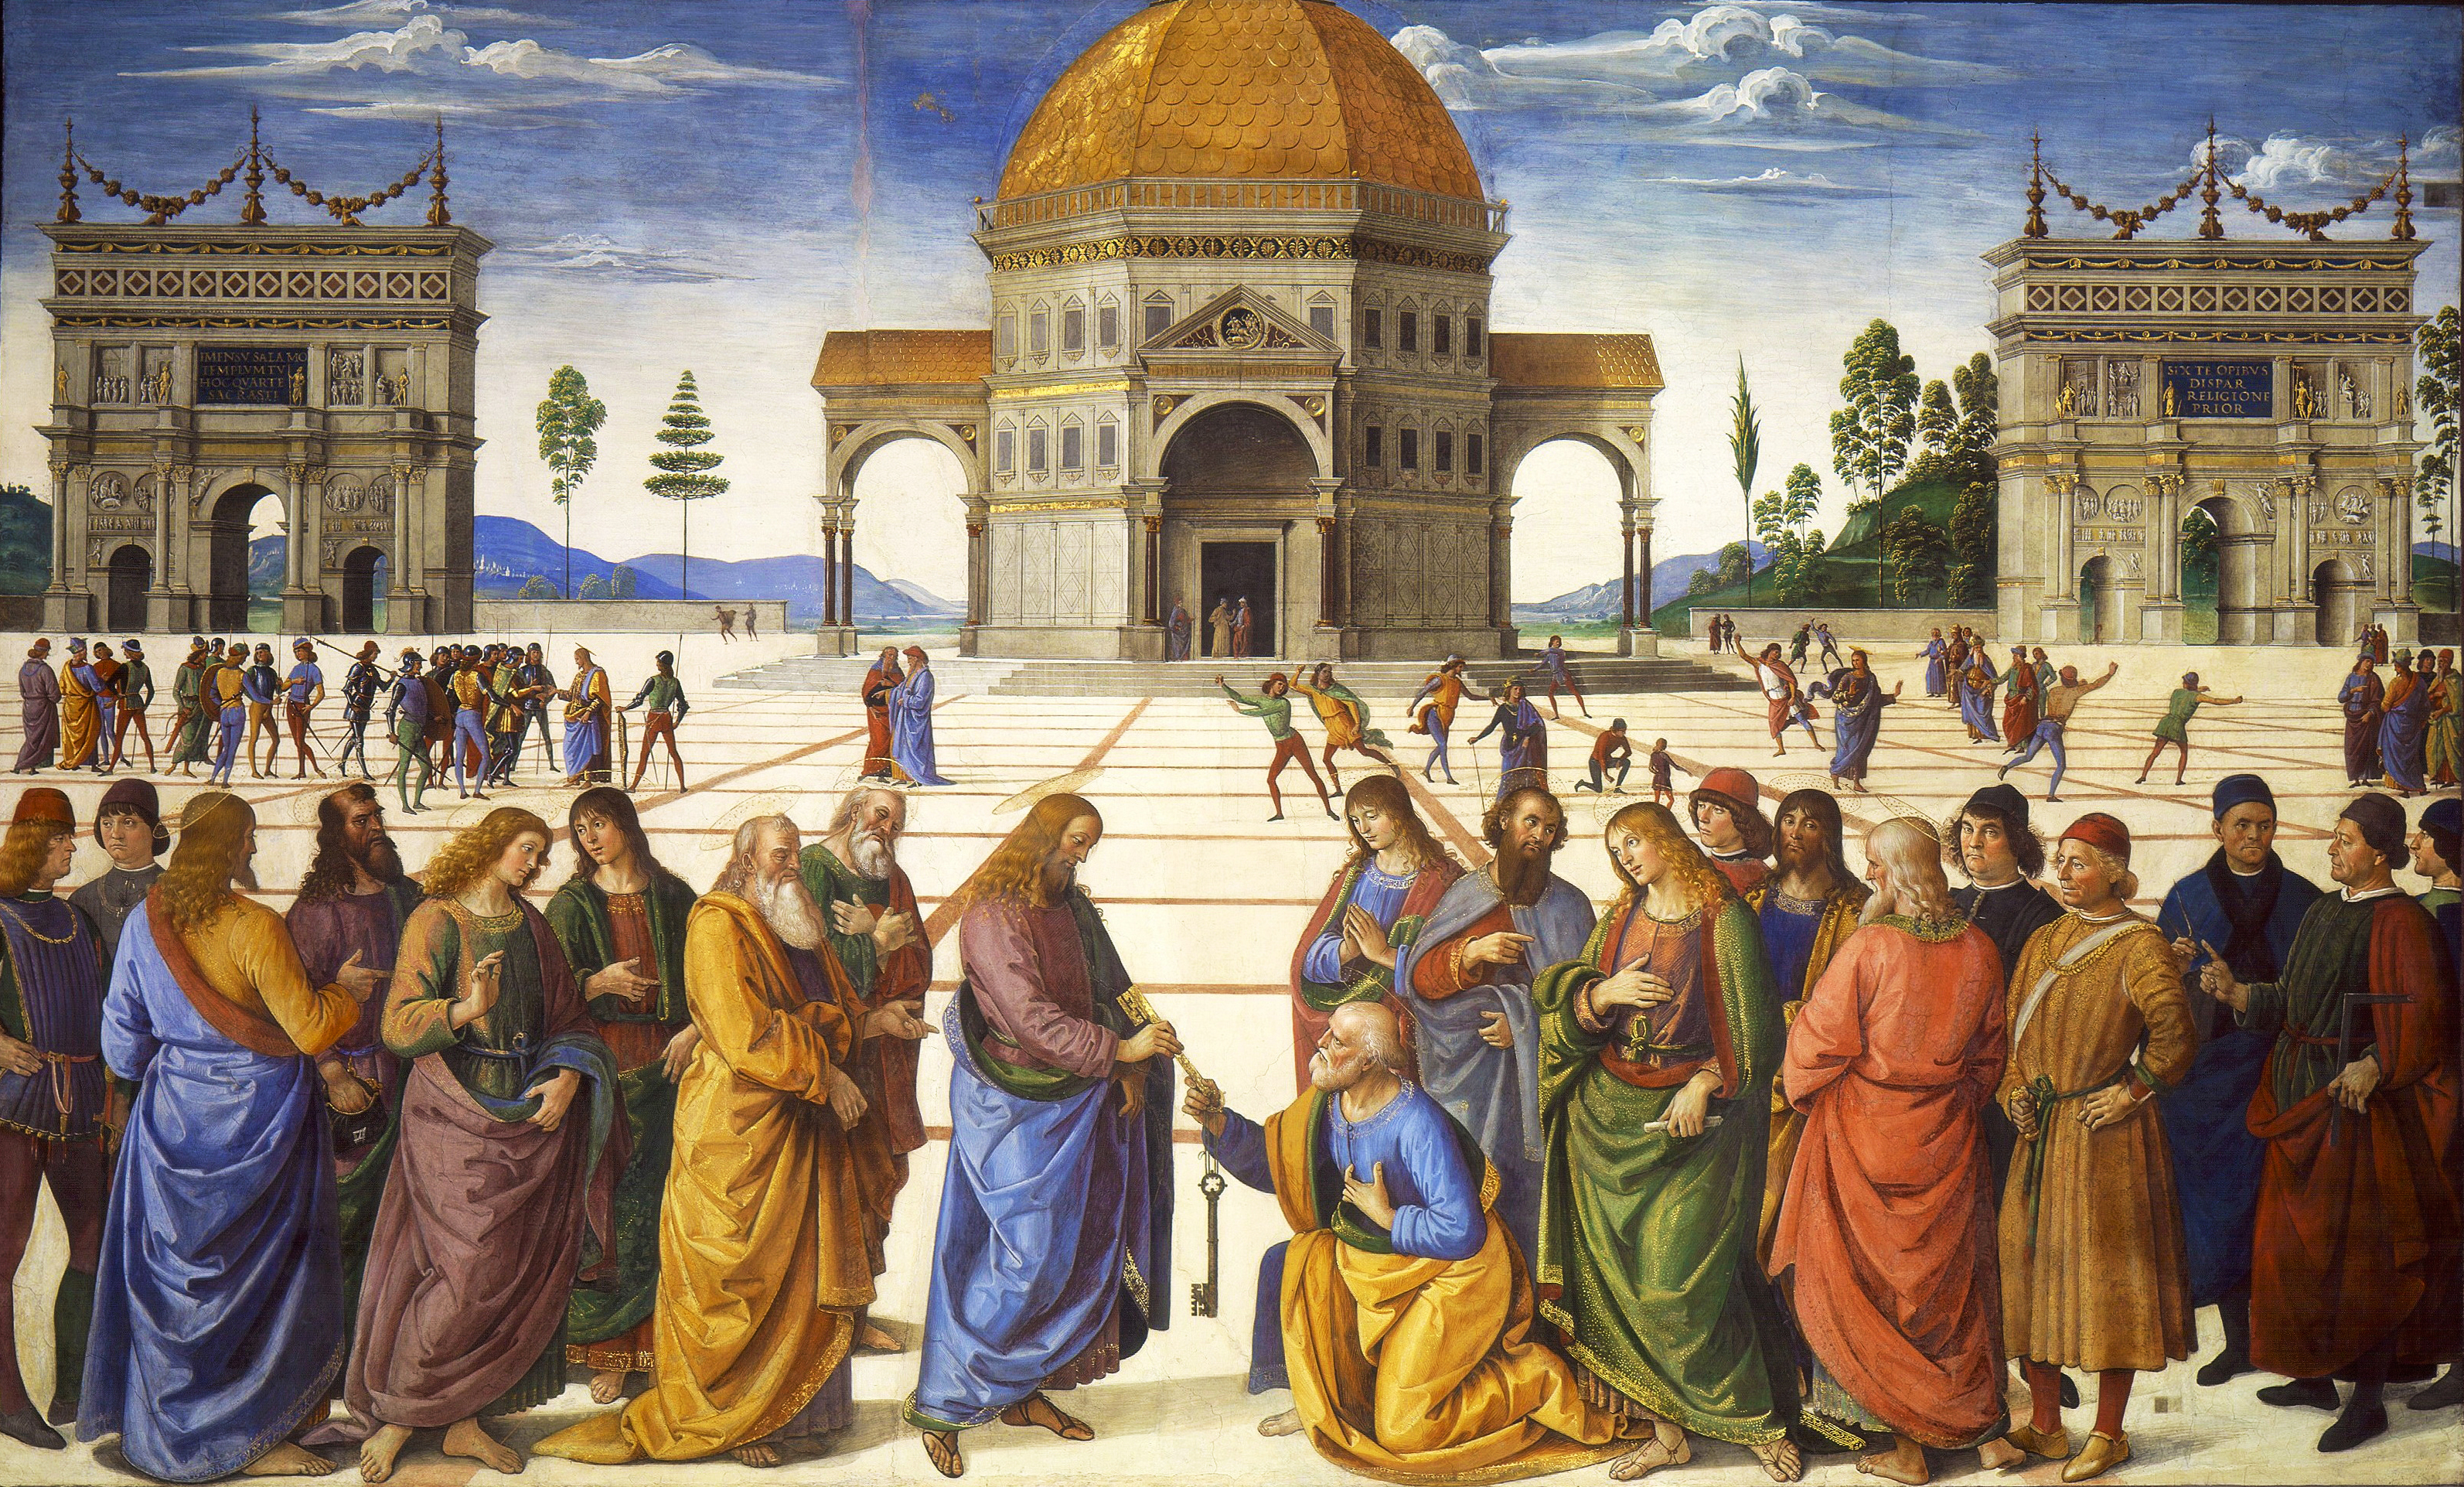
\includegraphics[width=.9\linewidth]{03.EstudioProblema/01.EstadoArte/00.Figuras/11.renacimiento_llaves_san_pedro.jpg}
  \captionof{figure}{Entrega de las llaves a San Pedro. Pietro Perugino. \cite{EA_img_llaves}}
  \label{fig:EA_llaves}
\end{minipage}
\end{figure}






\subsection{Siglo XIX}

Durante el siglo XIX se populariza en Europa el uso de imágenes panorámicas que ocupan los 360º de visión horizontal del espectador para transportarlo al lugar o evento representado. Comenzaron a crearse edificios de ocio dedicados a la presentación de imágenes panorámicas en los que los espectadores eran situados en el centro de una sala circular desde donde podían contemplar una o varias pinturas, normalmente de paisajes naturales, ciudades y zonas urbanas, así como grandes batallas militares, siendo una de las más populares el panorama de Londres de Robert Barker presentado en la figura \ref{fig:EA_london}.

El pintor Robert Barker fue el gran impulsor de este tipo de entretenimiento con su Rotunda en Leicester Square (véase figura \ref{fig:EA_rotunda}), donde exponía sus pinturas.



\begin{figure}
  \centering
\includegraphics[width=0.9\textwidth]{03.EstudioProblema/01.EstadoArte/00.Figuras/12.panorama_london.jpg}
    \caption{Panorama de Londres. \cite{EA_img_london}}
    \label{fig:EA_london}
\end{figure}

\begin{figure}
  \centering
\includegraphics[width=0.5\textwidth]{03.EstudioProblema/01.EstadoArte/00.Figuras/13.panorama_rotunda.jpg}
    \caption{Sección de la Rotunda en Leicester Square. \cite{EA_img_rotunda}}
    \label{fig:EA_rotunda}
\end{figure}


\label{par:estadoArte:estereoscopio}
En 1836 se descubre que el cerebro humano procesa por separado las imágenes de ambos ojos para crear una única imagen con profundidad debido a las ligeras diferencias entre la visión de cada ojo. Esto lleva al nacimiento de los primeros visores de imágenes estereoscópicas (figura \ref{fig:EA_estereoscopio}). En estos visores era posible insertar una serie de diferentes tarjetas que contenían dos imágenes tomadas con una cámara estereoscópica y permitían disfrutar de su visualización con una inmersión mayor a lo común para la época.


\begin{figure}
  \centering
\includegraphics[width=0.5\textwidth]{03.EstudioProblema/01.EstadoArte/00.Figuras/14.panorama_estereoscopico.jpg}
    \caption{Estereoscopio de David Brewster. \cite{EA_img_estereoscopio}}
    \label{fig:EA_estereoscopio}
\end{figure}




\subsection{Headsight}

En 1960 Morton Heilig creó el primer visor que se colocaba en la cabeza y permitía ver una película estereoscópica. Este dispositivo era muy limitado, pero en el año siguiente (1961) Philco Corporation creó el primer casco de realidad virtual con sensores de movimiento, el Headsight (figura \ref{fig:EA_headsight}). Headsight fue desarrollado para un uso militar y permitía al usuario controlar la rotación de una cámara de vigilancia según los movimientos de su cabeza mediante el uso de sensores magnéticos que controlaban la posición del visor.



\begin{figure}[H]
  \centering
\includegraphics[width=0.5\textwidth]{03.EstudioProblema/01.EstadoArte/00.Figuras/15.headsight.png}
    \caption{Headsight de Philco Corporation. \cite{EA_img_headsight}}
    \label{fig:EA_headsight}
\end{figure}



\subsection{Espada de Damocles}

En 1968 se dio un paso más hacia la realidad virtual que se conoce hoy en día. Ivan Sutherland y Bob Sproull tomaron la idea del Headsight y la transformaron de forma que en lugar de estar conectado una cámara de vigilancia se conectaría a un ordenador que generaría gráficos tridimensionales sencillos. Este dispositivo era tan grande y pesado que necesitaba ser sostenido del techo sobre el usuario, dándole así su nombre en referencia a la leyenda de Damocles en la cultura griega clásica. En la figura \ref{fig:EA_damocles} se puede comprobar el tamaño del dispositivo y su colocación sobre el usuario.


\begin{figure}[H]
  \centering
\includegraphics[width=0.5\textwidth]{03.EstudioProblema/01.EstadoArte/00.Figuras/16.damocles.jpg}
    \caption{Espada de Damocles de Ivan Sutherland y Bob Sproull. \cite{EA_img_damocles}}
    \label{fig:EA_damocles}
\end{figure}


\subsection{Realidad virtual}

A pesar de todos estos avances en la reproducción de una realidad artificial, no se disponía de un nombre y fue en 1987 cuando el término realidad virtual es definido por Jaron Lanier un informático y compositor estadounidense. Tras fundar una compañía llamada Visual Programming Lab, diseñó y desarrolló los que serían los primeros dispositivos de realidad virtual disponibles para ser adquiridos por el público: el EyePhone y el Dataglove, un visor y un guante para interactuar con el espacio virtual.

Pese al gran avance que suponen estos productos, la tecnología aún tenía mucho por mejorar. El sistema del EyePhone junto con el ordenador necesario para generar las imágenes del mundo virtual costaban hasta 250.000 dólares, y aun así solo eran capaces de alcanzar una tasa de imágenes de 5 fotogramas por segundo, una cifra insuficiente para ofrecer una experiencia fluida al usuario.

Este visor contenía elementos nunca vistos en el ámbito de la realidad virtual. Utilizaba sensores capaces de reconocer las expresiones faciales del usuario, todos los sonidos eran procesados por el ordenador para darles un efecto 3D de forma que su fuente se movía por el espacio dependiendo de los movimientos de la cabeza del usuario. El Dataglove solo era capaz de transmitir sensaciones hápticas al usuario si no que también actuaba como sensor, pudiendo generar en el espacio virtual un modelo de la mano del usuario que éste podía utilizar para interactuar con el ambiente.

A pesar de que este dispositivo fue el primero que se asemejaba a la visión actual de un visor de realidad virtual, requería de una gran potencia informática para la época, resultando en un producto demasiado caro y voluminoso, como se puede ver en la figura \ref{fig:EA_eyePhone}.




%\begin{figure}
%\centering
%\begin{minipage}{.5\textwidth}
%  \centering
%  \includegraphics[width=.9\linewidth]{03.EstudioProblema/01.EstadoArte/00.Figuras/eyephone.jpg}
%  \captionof{figure}{Demostración de EyePhone y Dataglove.
%. \cite{EA_img_eyePhone}}
%  \label{fig:EA_eyePhone}
%\end{minipage}%
%\begin{minipage}{.5\textwidth}
%  \centering
%  \includegraphics[width=.9\linewidth]{03.EstudioProblema/01.EstadoArte/00.Figuras/eyephoneDataglove.jpg}
%  \captionof{figure}{Dataglove siendo usado por Chad Leeper durante una conferencia.
%. \cite{EA_img_dataglobe}}
%  \label{fig:EA_dataglobe}
%\end{minipage}
%\end{figure}

\begin{figure}[H]
  \centering
\includegraphics[width=0.5\textwidth]{03.EstudioProblema/01.EstadoArte/00.Figuras/17.eyephone_dataglove.jpg}
    \caption{Eyephone y Dataglove junto al sistema de seguimiento Polhemus en exposición Nissho Iwai en Tokio en 1999. \cite{EA_img_eyePhone}}
    \label{fig:EA_eyePhone}
\end{figure}


\subsection{Virtual Boy}

En 1995 la compañía de videojuegos japonesa Nintendo lanza al mercado su Virtual Boy, la primera consola portátil con gráficos verdaderamente tridimensionales (figura \ref{fig:EA_virtualBoy}). Esta consola prometía ser un gran éxito, pero acabó siendo un fracaso. Su precio, aun siendo más asequible que el EyePhone, seguía siendo elevado para lo que ofrecía: 180 dólares.

La Virtual Boy disponía de dos matrices lineales de láser de 1x224 que escaneaban constantemente el campo visual de cada ojo con la ayuda de dos espejos que oscilaban rápidamente. Por esto, la consola emitía un constante murmuro mientras estaba en uso.

La consola solo podía reproducir un único color, junto con el negro. Se escogió el color rojo por las características de los LED de este color: son más baratos y consumen menos energía que otros colores.

Esta consola utilizaba un procesador NEC V810 de arquitectura RISC y 32 bit a 20MHz, que era acompañado de 1MB de memoria RAM. La resolución efectiva de las pantallas era de 384x224 píxeles. Toda la consola era alimentada a partir de 6 pilas AA situadas en el mando.

Por desgracia, el uso prolongado de este dispositivo causaba dolores de cabeza y mareos, que, junto con su pequeña y básica selección de juegos (entre ellos, el más popular: Mario's Tennis, representado en la figura \ref{fig:EA_virtualBoyJuego}), llevaron a que la consola fuera descontinuada menos de un año después de su lanzamiento.



\begin{figure}
\centering
\begin{minipage}{.5\textwidth}
  \centering
  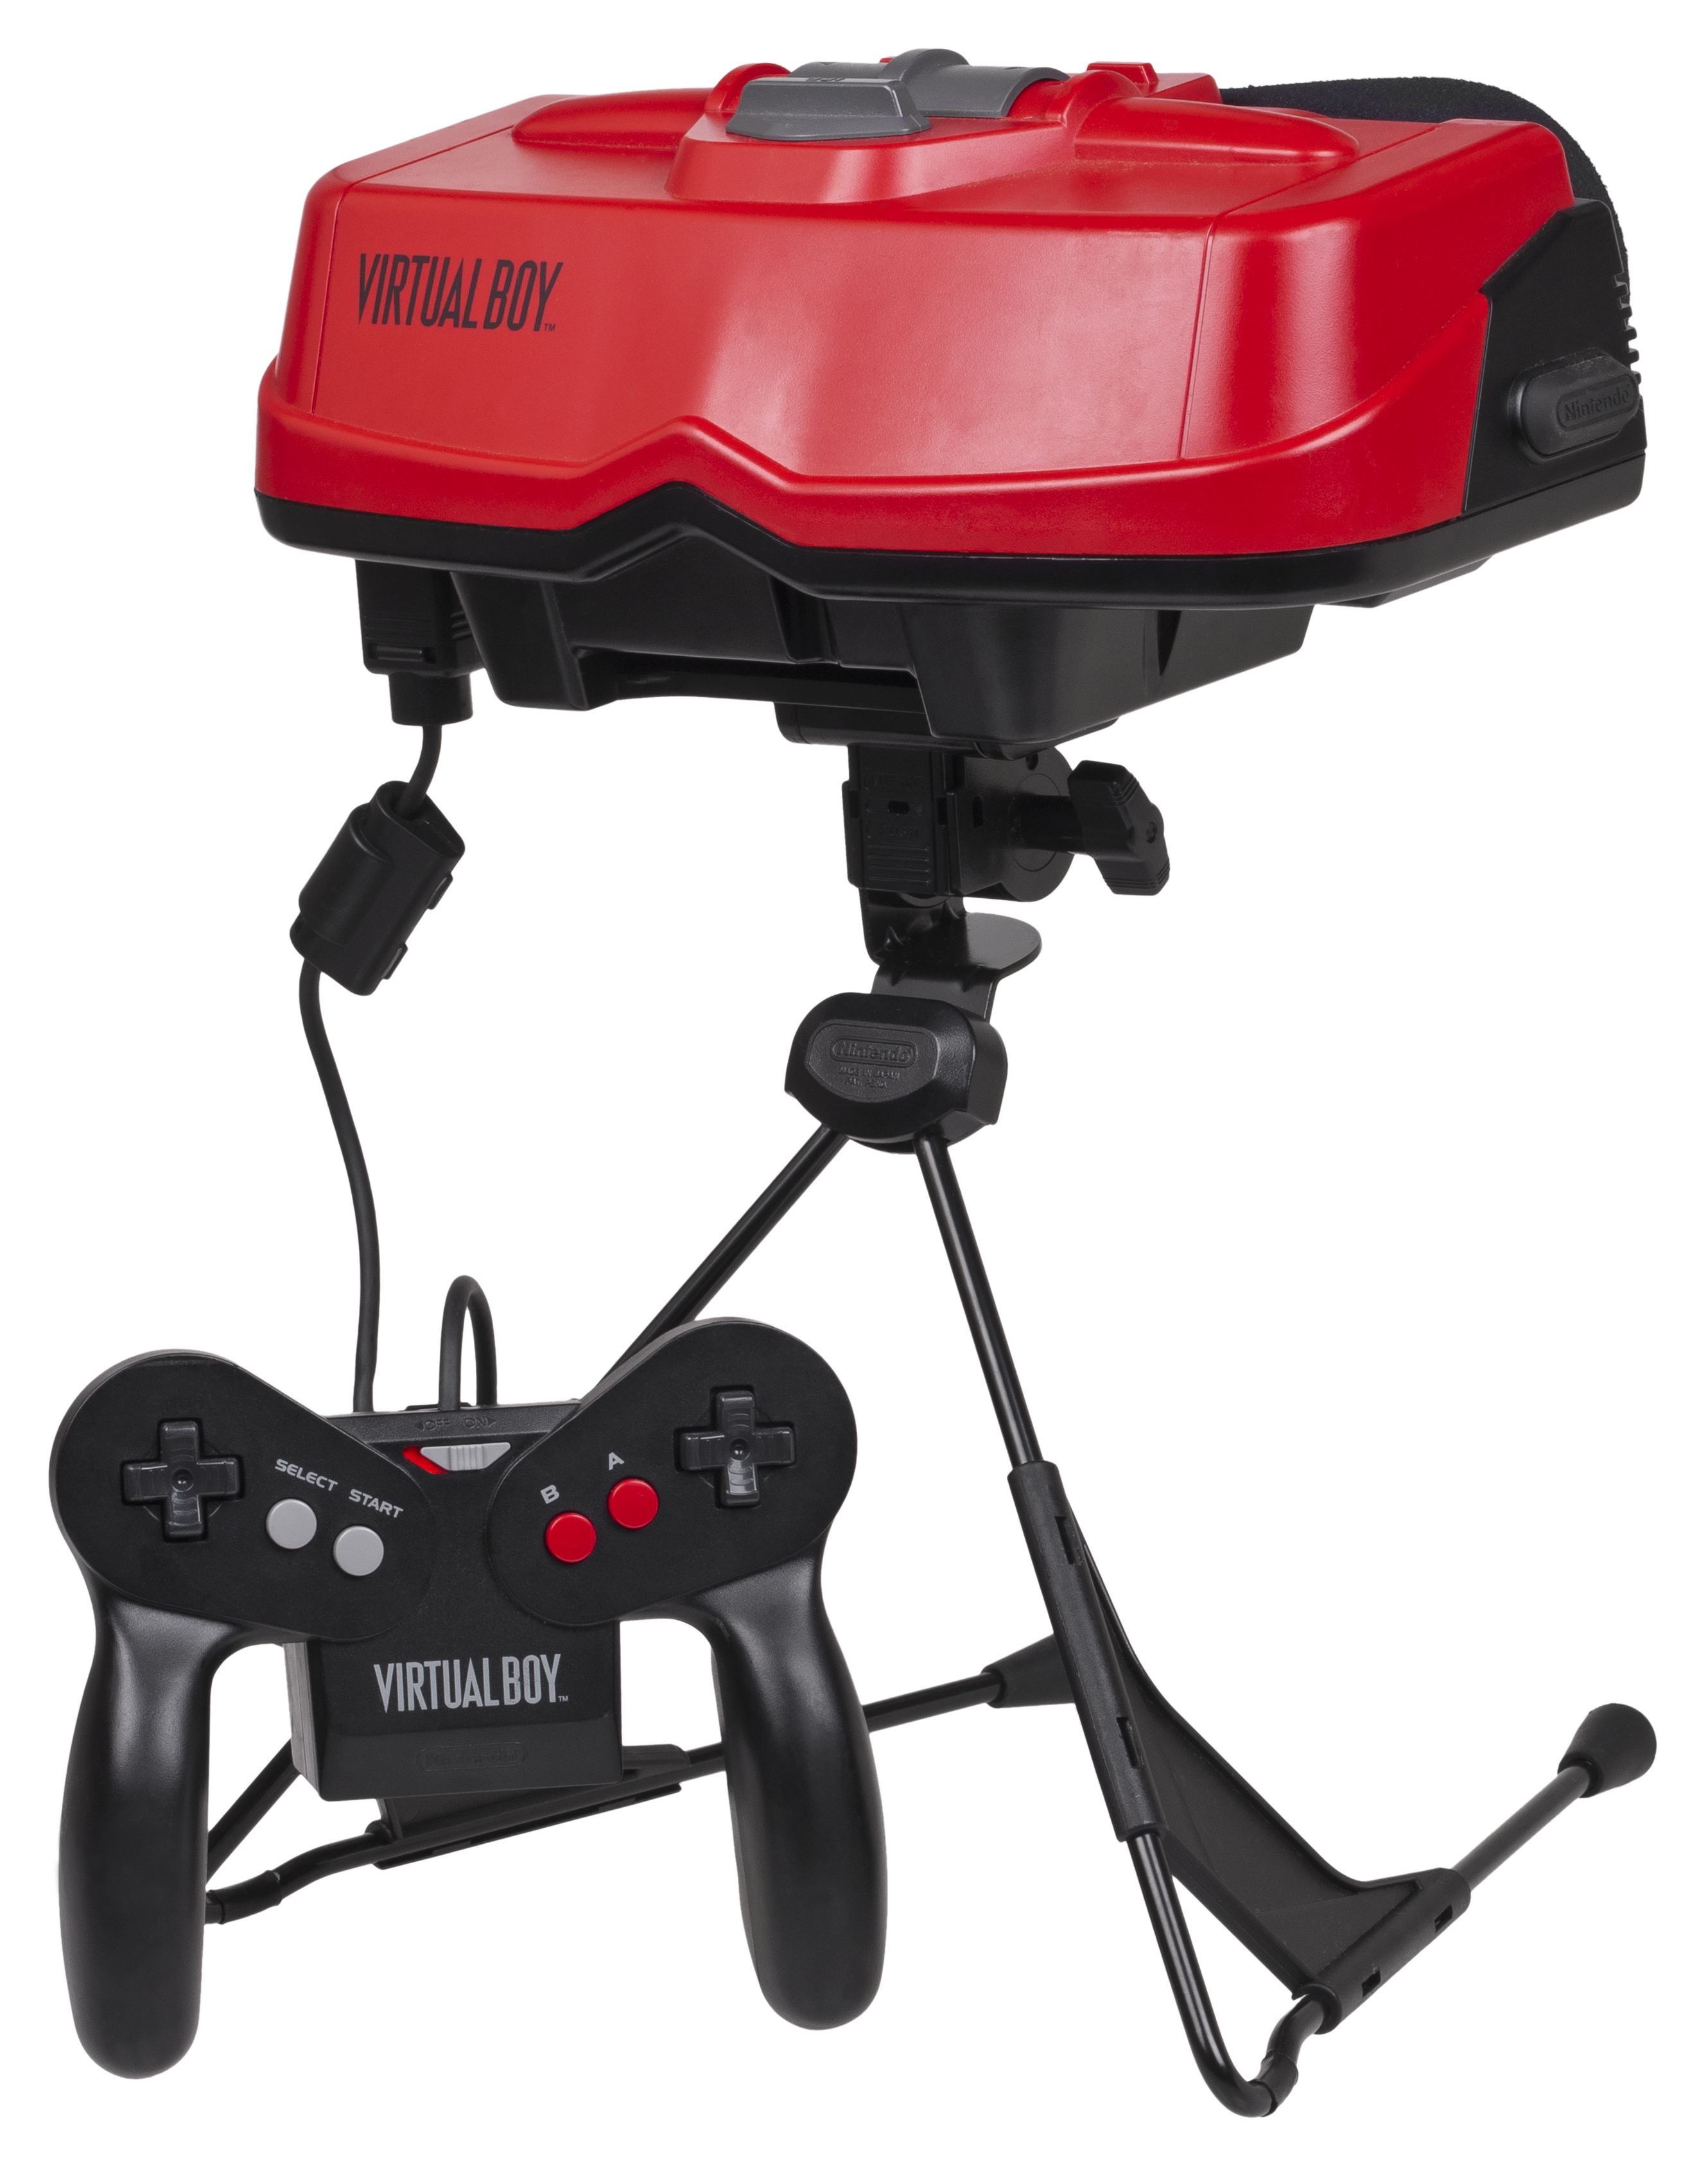
\includegraphics[width=.7\linewidth]{03.EstudioProblema/01.EstadoArte/00.Figuras/18.virtualboy.png}
  \captionof{figure}{Virtual Boy de Nintendo. \cite{EA_img_virtualBoy}}
  \label{fig:EA_virtualBoy}
\end{minipage}%
\begin{minipage}{.5\textwidth}
  \centering
  \includegraphics[width=.9\linewidth]{03.EstudioProblema/01.EstadoArte/00.Figuras/19.marios_tennis.png}
  \captionof{figure}{Mario's Tennis. Videojuego de Nintendo para Virtual Boy. \cite{EA_img_virtualBoyJuego}}
  \label{fig:EA_virtualBoyJuego}
\end{minipage}
\end{figure}



\subsection{Siglo XXI}

En los últimos años ha habido un crecimiento acelerado de la tecnología: los ordenadores han multiplicado su potencia y capacidad de procesamiento paralelo, los dispositivos móviles se han vuelto mucho más sofisticados que cualquier ordenador del siglo XX, las pantallas son capaces de reproducir millones de colores a altas frecuencias de refresco y el acceso a Internet de alta velocidad es algo común. Estos avances han hecho resurgir con más fuerza que nunca la realidad virtual, especialmente en el ámbito de los videojuegos.

En 2010, el joven empresario Palmer Luckey creó el prototipo de un casco de realidad virtual al que llamó Oculus Rift, véase la figura \ref{fig:EA_kitOculus}. Este dispositivo podía representar imágenes de alta resolución con un campo de visión de 90º, algo muy superior a lo existente hasta el momento. Dos años después, Oculus Rift logró financiación a partir de una campaña de micro financiación.


\begin{figure}
  \centering
\includegraphics[width=0.5\textwidth]{03.EstudioProblema/01.EstadoArte/00.Figuras/20.oculus_rift_dk1.jpg}
    \caption{Primer kit de desarrollo de Oculus Rift. \cite{EA_img_kitOculus}}
    \label{fig:EA_kitOculus}
\end{figure}



Entre los años 2014 y 2015 se produjo un boom en la realidad virtual de consumo, apareciendo muchas alternativas para el público general:

\begin{itemize}
	\item{Sony anuncia PlayStation VR un casco de RV para su consola PlayStation 4. Figura \ref{fig:EA_psvr}.}

	\item{Samsung lanza al mercado su Samsung Gear VR, un visor que utiliza un smartphone (Samsung Galaxy) como centro de procesamiento y pantalla.}

	\item{Google produce las Google Cardboard, una alternativa barata que permite al usuario crear su propio visor y utilizar su propio dispositivo móvil con Android como pantalla. Figura \ref{fig:EA_cardboard}.}

\end{itemize}


\begin{figure}
  \centering
\includegraphics[width=0.5\textwidth]{03.EstudioProblema/01.EstadoArte/00.Figuras/21.psvr.png}
    \caption{PlayStation VR. \cite{EA_img_psvr}}
    \label{fig:EA_psvr}
\end{figure}

\begin{figure}
  \centering
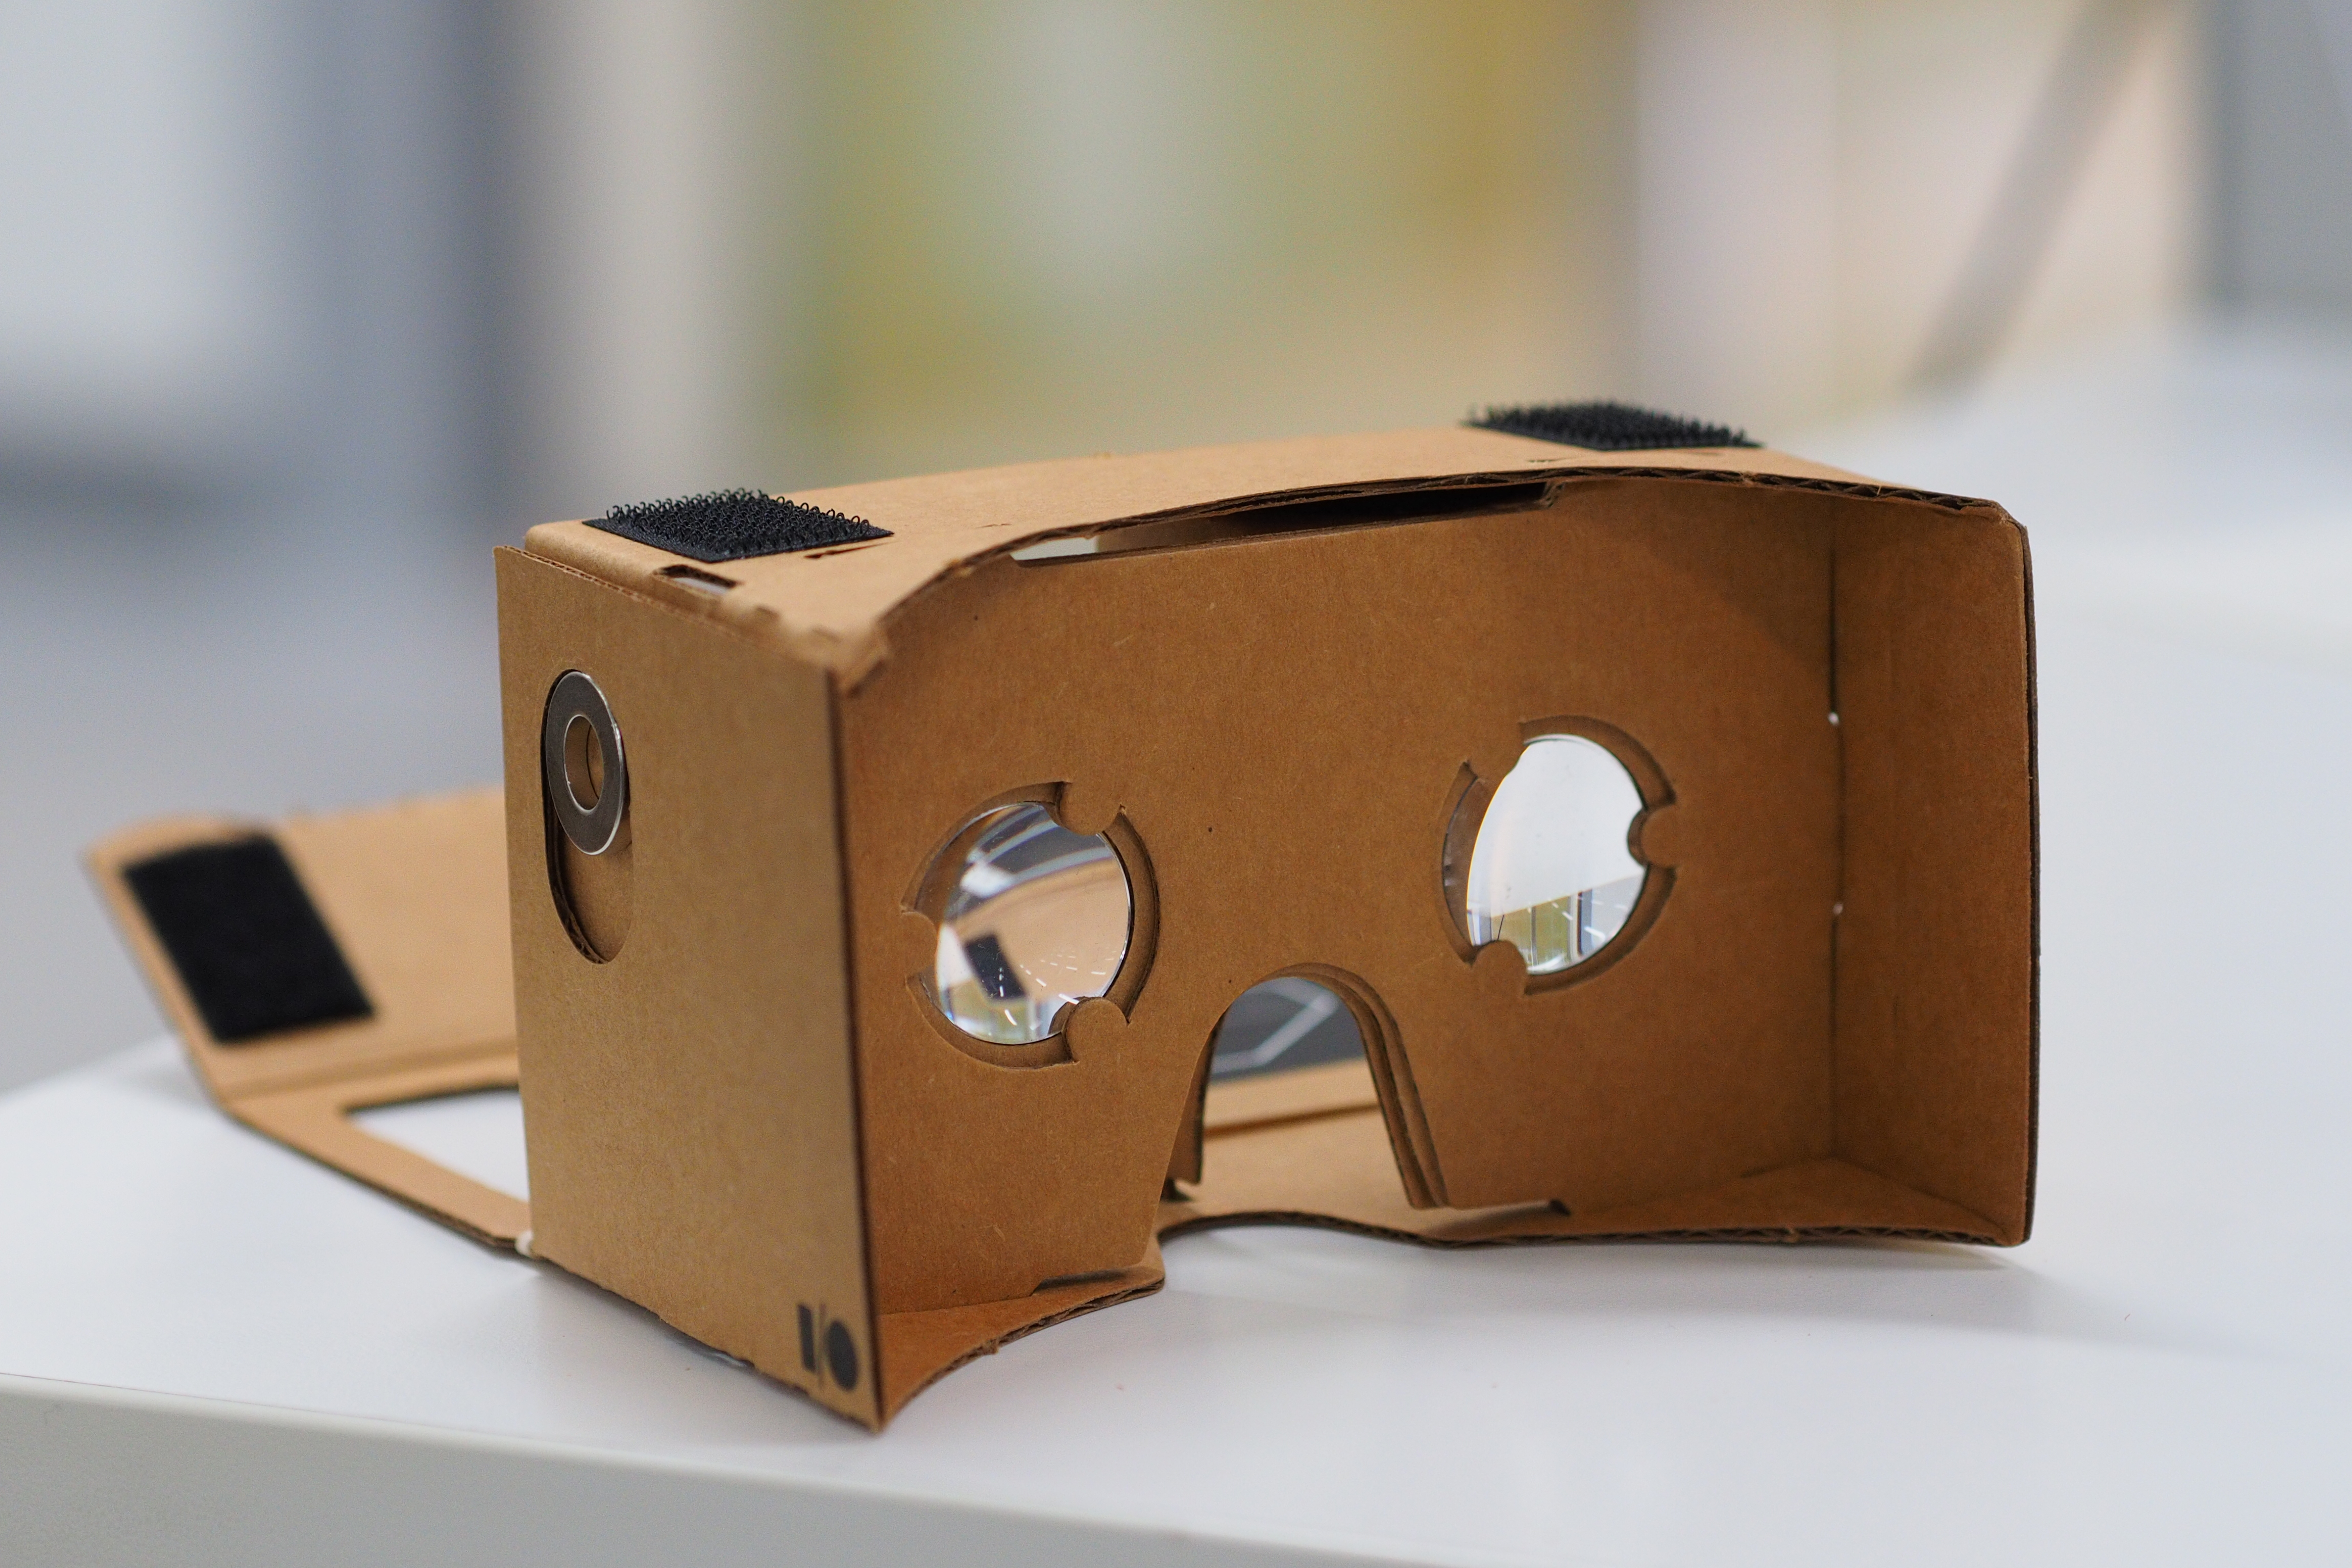
\includegraphics[width=0.5\textwidth]{03.EstudioProblema/01.EstadoArte/00.Figuras/22.cardboard.jpg}
    \caption{Google Cardboard ensamblada. \cite{EA_img_cardboard}}
    \label{fig:EA_cardboard}
\end{figure}


Con la aparición de dispositivos capaces de reproducir contenido de realidad virtual, también fueron apareciendo videojuegos y otras experiencias para los mismos. La RV era ya una parte fundamental del ocio y los videojuegos.

En 2016 se lanza al mercado HTC Vive, un completo sistema de realidad virtual (véase figura \ref{fig:EA_vive}) producido en colaboración entre HTC y Valve, productores de hardware y software respectivamente. El HTC Vive pasó a ser el casco de RV de referencia en el sector: contaba con pantallas OLED de alta resolución (1080x1200 píxeles) y tasa de refresco de 90Hz que ofrecían un campo de visión de 110º, contaba con dos mandos de control táctiles con respuesta háptica, así como un sistema de sensores colocados en la habitación que permitían definir un espacio de juego de hasta 25 m2 en el que el jugador podía moverse libremente.


\begin{figure}
  \centering
\includegraphics[width=0.5\textwidth]{03.EstudioProblema/01.EstadoArte/00.Figuras/23.htc_vive.jpeg}
    \caption{HTC Vive y todos sus complementos. \cite{EA_img_vive}}
    \label{fig:EA_vive}
\end{figure}


\subsection{Actualidad}


Actualmente, en el año 2019, la realidad virtual continua sin ser perfecta pero también continúa mejorando cada día. A pesar de no ser el más avanzado tecnológicamente, el dispositivo de Sony (PSVR) ha tenido una gran aceptación entre el público debido a su menor precio y especialmente a la enorme acogida de la consola PlayStation 4. Incluso 3 años después de su salida al mercado, y de las nuevas opciones disponibles, PSVR continúa siendo el dispositivo de realidad virtual más vendido en el mundo con 2.2 millones de unidades vendidas frente a los 1.7 millones de su competidor más cercano: Oculus.

En este último año, además, se han originado dos enfoques para la RV claramente diferenciados y liderados por dos empresas principalmente: Valve y Oculus.

En verano de 2019 Valve lanza al mercado un nuevo producto. Tras romper su alianza comercial con HTC, Valve desarrolla su propio visor de RV llamado Valve Index, mostrado en la figura \ref{fig:EA_index}. Este dispositivo mejora en todos los aspectos a su predecesor, el HTC Vive:


\begin{itemize}
	\item{Dispone de pantallas OLED de 1440x1600 píxeles con refresco de hasta 144Hz.}

	\item{Dos cámaras estereoscópicas situadas al frente del dispositivo permiten su uso durante el juego como cámaras de video o como sensores.}

	\item{Los mandos de control han sido mejorados y ahora son capaces de detectar movimientos de cada dedo individualmente gracias a sensores de proximidad.}
	
	\item{Las nuevas estaciones (sensores colocados en la habitación) ahora permiten un campo de juego de hasta 100m2 comparados con los 25m2 del HTC Vive.}

\end{itemize}


\begin{figure}
  \centering
\includegraphics[width=0.5\textwidth]{03.EstudioProblema/01.EstadoArte/00.Figuras/24.valve_index.jpg}
    \caption{Kit de visor Valve Index junto a controles y estaciones base. \cite{EA_img_index}}
    \label{fig:EA_index}
\end{figure}



Pero todas estas mejoras conllevan un gran coste y el precio del kit completo asciende hasta 1080 euros en su lanzamiento. A este precio habrá que sumar el precio de un ordenador con capacidad suficiente para ejecutar los videojuegos tan demandantes que están diseñados para este dispositivo.

Por otra parte, Oculus lanza su nuevo producto un mes antes que el Valve Index, pero con una mentalidad completamente diferente: en lugar de buscar la máxima potencia e innovación tecnológica, se busca una mayor portabilidad y eficiencia manteniendo el coste bajo para que sea accesible por un mercado más amplio. Este nuevo dispositivo es el Oculus Quest. Este visor no se conecta a un ordenador para reproducir los videojuegos, si no que se trata de un visor de RV completamente independiente. Véase figura \ref{fig:EA_oculusQuest}.

Oculus Quest contiene un sistema Android personalizado que se ejecuta sobre un procesador ARM de 8 núcleos Cortex-A73 (4 núcleos Kryo 208 Gold a 2.45GHz y 4 Kryo 280 Silver a 1.9GHz) y un procesador gráfico Adreno 540, que están acompañados de 4GB de memoria RAM y hasta 128GB de almacenamiento. Tiene dos pantallas OLED de 1440x1600 píxeles similares a las del Valve Index, pero funcionan solo 72Hz.


\begin{figure}
  \centering
\includegraphics[width=0.5\textwidth]{03.EstudioProblema/01.EstadoArte/00.Figuras/25.meta_quest_2.jpg}
    \caption{Oculus Quest. \cite{EA_img_oculusQuest}}
    \label{fig:EA_oculusQuest}
\end{figure}


Este dispositivo no depende de estaciones de sensores fijas en la habitación ya que es capaz de generar la zona de juego a partir de los sensores que lleva incorporados el propio visor. Debido a esto aparecen nuevas restricciones en los mandos: para que estos funcionen de forma adecuada deberán estar situados delante del visor, si el usuario hace un movimiento demasiado amplio, los mandos saldrán de la zona captada por los sensores y dejarán de ser reconocidos.

Pese a ser un visor más limitado que el Valve Index, la portabilidad y precio del Oculus Quest hacen que sea uno de los visores de RV más para tener en cuenta en la actualidad.





\section{Motores de videojuegos}

Para diseñar y desarrollar videojuegos, ya sean de tipo brain training o cualquier otro, se utiliza habitualmente un motor de juego.

Un motor de juego es un entorno de trabajo o framework que contiene funcionalidades básicas para la creación de videojuegos como: un motor de físicas, renderizado de gráficos, gestor de comunicación en red o comunicaciones a bajo nivel con el hardware en el que se ejecutará el videojuego. Por tanto, un motor de juego provee de una base sobre la que desarrollar un videojuego de forma más ágil, ahorrando tiempo, esfuerzo y dinero.

\subsection{Unity}

Es un motor capaz de crear videojuegos multiplataforma de multitud de géneros de manera sencilla. Es el motor más utilizado por desarrolladores independientes debido a su bajo coste y a su gran comunidad de desarrolladores online y su gran documentación. Figura \ref{fig:EA_interfazUnity}.


\begin{figure}[H]
  \centering
\includegraphics[width=0.8\textwidth]{03.EstudioProblema/01.EstadoArte/00.Figuras/26.interfaz_unity.jpg}
    \caption{Interfaz de Unity. \cite{EA_img_interfazUnity}}
    \label{fig:EA_interfazUnity}
\end{figure}


Destaca en la creación de videojuegos para plataformas móviles. Con este motor se ha desarrollado juegos como Ori and the Blind Forest, Hollow Knight, Monument Valley 2 (figura \ref{fig:EA_monumentValley}), Kerbal Space Program o Firewatch.

Unity cuenta con un plan personal completamente gratuito y libre de regalías. Pero en caso de que la recaudación del juego supere los 100.000 dólares al año se deberá adquirir un plan de pago mensual de entre 40 y 150 dólares. En caso de superar los 200.000\$ de ingresos o contar con más de 3 trabajadores, se deberá contratar un plan empresarial propuesto por Unity.





\begin{figure}[H]
  \centering
\includegraphics[width=0.6\textwidth]{03.EstudioProblema/01.EstadoArte/00.Figuras/27.monument_valley_2.jpg}
    \caption{Monument Valley 2. \cite{EA_img_monumentValley}}
    \label{fig:EA_monumentValley}
\end{figure}


\subsection{Unreal Engine}

Actualmente es uno de los motores más utilizados por su potencia y acabados gráficos, así como permitir trabajar para distintas plataformas, entre ellas PC, PS4, Xbox One, Nintendo Switch, Android o iOS. Fue creado por la empresa Epic Games, desarrolladora de juegos como Fortnite y la serie Unreal. Figura \ref{fig:EA_interfazUnreal}.

\begin{figure}[H]
  \centering
\includegraphics[width=0.8\textwidth]{03.EstudioProblema/01.EstadoArte/00.Figuras/28.interfaz_unreal.png}
    \caption{Interfaz de Unreal Engine 4. \cite{EA_img_interfazUnreal}}
    \label{fig:EA_interfazUnreal}
\end{figure}

Unreal Engine permite un elevado grado de personalización, lo que hace que pueda usarse para crear juegos de multitud de géneros diferentes: Aventura, FPS, lucha 2D, puzles, etc.

Este motor ha sido utilizado para crear los videojuegos de la saga Gears of War, Bioshock, Kingdom Hearts III y Fortnite (figura \ref{fig:EA_fortnite}) entre muchos otros.

Este motor presenta un modelo de negocio basado en regalías, de modo que su uso es completamente gratuito, pero a cambio Epic Games recibirá un 5\% de los ingresos del juego en caso de que este supere los 3000 dólares de beneficio en un trimestre.




\begin{figure}[H]
  \centering
\includegraphics[width=0.8\textwidth]{03.EstudioProblema/01.EstadoArte/00.Figuras/29.fortnite.jpg}
    \caption{Visión del jugador durante una partida de Fortnite. \cite{EA_img_fortnite}}
    \label{fig:EA_fortnite}
\end{figure}





\subsection{Game Maker}

Este motor tiene la particularidad de que no requiere conocimientos extensos en programación, si no que permite usar una interfaz para seleccionar y arrastrar una serie de acciones predefinidas y de esta forma crear los eventos que formarán el juego. Además de esta interfaz, también permite el uso de su propio lenguaje GML para la programación en profundidad de los eventos. Estas características lo hacen un motor ideal para aquellas personas con conocimientos limitados en el campo de la informática. Figura \ref{fig:EA_gameMaker}.

\begin{figure}[H]
  \centering
\includegraphics[width=0.8\textwidth]{03.EstudioProblema/01.EstadoArte/00.Figuras/30.interfaz_game_maker.jpg}
    \caption{Interfaz de GameMaker Studio 2. \cite{EA_img_gameMaker}}
    \label{fig:EA_gameMaker}
\end{figure}

Sin embargo, este motor es mucho más limitado que los anteriores en la lista, tanto en capacidad y rendimiento, como en variedad de géneros que puede abarcar, estando limitado a los gráficos 2D o 3D muy básicos. A pesar de estas limitaciones, su versión más reciente (GameMaker Studio 2) permite la distribución en prácticamente todas las plataformas habituales en la actualidad.

GameMaker sigue un modelo de pago anual con posibilidad de realizar una prueba gratuita de 30 días. Una vez terminada la prueba, se deberá adquirir una licencia, que va desde los 39\$ al año para la versión más básica que solo permite publicar en una plataforma: Windows o MacOs. Y los precios aumentan por cada nueva plataforma en la que se quiera publicar: 149\$ para web, 200\$ para Android y iOS, o 799\$ por cada una de las consolas de sobremesa (PS4, Xbox One y Nintendo Switch).

Debido a su facilidad de uso y la no necesidad de conocimientos profundos de informática, es un motor que muchos desarrolladores independientes utilizan para sus juegos. Por ejemplo, para juegos como Crashlands (figura \ref{fig:EA_crashlands}), Hyper Light Drifter o Forager.



\begin{figure}
  \centering
\includegraphics[width=0.8\textwidth]{03.EstudioProblema/01.EstadoArte/00.Figuras/31.crashlands.jpg}
    \caption{Captura de pantalla de Crashlands. \cite{EA_img_crashlands}}
    \label{fig:EA_crashlands}
\end{figure}


\subsection{Godot}

Este motor es el único de la lista que es completamente gratuito y de código abierto. Permite crear todo tipo de videojuegos tanto en 2D como en 3D y además tiene una gran comunidad de desarrolladores en Internet, haciéndolo uno de los motores más fáciles de usar a la vez que versátiles. Figura \ref{fig:EA_godot}.

Godot engine soporta la creación de juegos para PC y dispositivos móviles como Oddventure o RivenTails: Defense (figura \ref{fig:EA_rivenTails}), sin embargo, su soporte para consolas de sobremesa es limitado y no oficial.


\begin{figure}[H]
  \centering
\includegraphics[width=0.8\textwidth]{03.EstudioProblema/01.EstadoArte/00.Figuras/32.interfaz_godot.png}
    \caption{Interfaz de Godot en modo web. \cite{EA_img_godot}}
    \label{fig:EA_godot}
\end{figure}

\begin{figure}[H]
  \centering
\includegraphics[width=0.8\textwidth]{03.EstudioProblema/01.EstadoArte/00.Figuras/33.riventails_defense.jpg}
    \caption{Captura de pantalla de RivenTails: Defense. \cite{EA_img_rivenTails}}
    \label{fig:EA_rivenTails}
\end{figure}




\section{Conclusión y justificación del proyecto}


La importancia de los ejercicios de brain training para mantener en buen estado las capacidades cognitivas de las personas es evidente, y por ello estos ejercicios han ido evolucionando y cambiando para adaptarse a los distintos medios disponibles. En la actualidad se puede acceder a estos ejercicios desde multitud de dispositivos desde la comodidad del salón. Sin duda esto ha supuesto una mejora en la calidad de vida de muchas personas y de una forma amigable y entretenida, ya que las nuevas tecnologías no solo facilitan el acceso a los ejercicios, si no que los pueden mejorar en gran medida. 

El uso de vídeos, programas interactivos o animaciones coloridas resulta en ejercicios mucho más atractivos para el usuario, que no los verá como una carga o un proceso tedioso, si no como un juego entretenido y divertido. A pesar de esto, los ejercicios actuales tienen raíz en los ejercicios tradicionales y son una evolución directa de los mismos, heredando algunas de sus limitaciones. 

La evolución de la realidad virtual permite que hoy en día puedan crearse experiencias mucho más inmersivas e interactivas que cualquier otra tecnología que utilice una pantalla y métodos de control normales. Aunque en la actualidad existen algunas pruebas utilizando RV aplicada al entrenamiento cognitivo, sigue siendo un campo sin aprovechar completamente.

Es especialmente importante destacar que el entrenamiento cognitivo tiene un componente lúdico que es muy importante aprovechar para mantener al usuario motivado y con ánimo. De igual forma, la realidad virtual no es algo puramente recreativo; puede usarse y se usa con otros propósitos, especialmente en medicina, donde se pueden utilizar modelos 3D de pacientes reales para diagnosticar enfermedades o evaluar intervenciones quirúrgicas incluso antes de realizarlas.

Por este motivo, este proyecto busca complementar la parte lúdica de los ejercicios con el componente serio de la realidad virtual, intentando crear un videojuego que sea capaz de sacar todo el partido a ambos campos.

Por supuesto, esto no sería posible sin la proliferación en popularidad del videojuego, que lo ha convertido en un medio de gran importancia, dando lugar a la creación de motores de videojuegos disponibles para el público, que permiten el desarrollo de videojuegos independientes.



\chapterend


% Análisis inicial.
%%%%%%%%%%%%%%%%%%%%%%%%%%%%%%%%%%%%%%%%%%%%%%%%%%%%%%%%%%%%%%%%%%%
%%% Documento LaTeX 																						%%%
%%%%%%%%%%%%%%%%%%%%%%%%%%%%%%%%%%%%%%%%%%%%%%%%%%%%%%%%%%%%%%%%%%%
% Título:		Introducción
% Autor:  	Ignacio Moreno Doblas
% Fecha:  	2014-02-01, actualizado 2019-11-11
% Versión:	0.5.0
%%%%%%%%%%%%%%%%%%%%%%%%%%%%%%%%%%%%%%%%%%%%%%%%%%%%%%%%%%%%%%%%%%%
% !TEX root = A0.TFG.tex

\chapterbegin{Análisis inicial del problema}
\minitoc


Para alcanzar el objetivo de este proyecto se va a desarrollar un videojuego del género de concursos, en el que el jugador tendrá que resolver una serie de pruebas de diferentes categorías. En el desarrollo de videojuegos se suele crear un Documento de Diseño de Juego (GDD por sus siglas en inglés) de forma previa al inicio del desarrollo. En éste se documentan todas las ideas y planificaciones para tener en cuenta durante el desarrollo del videojuego, incluyendo personajes, historia, mecánicas, público objetivo o plataforma. 

Para el desarrollo de este proyecto también se ha creado un GDD, que se encuentra añadido a esta memoria en el apéndice \ref{sec:apendice:GDD}.

Este videojuego es ante todo un juego serio, es decir, su principal propósito no es el de entretener, si no el de permitir al jugador entrenar sus habilidades cognitivas. Eso no quiere decir que el juego no contenga una parte lúdica destinada a entretener al usuario y hacer el juego divertido. En este caso, el videojuego estará ambientado en un plató de televisión para concursos similar al mostrado en la figura \ref{fig:AI_atrapaMillon}, tomando una estructura similar a dichos concursos. 

El jugador se encontrará en el centro de un plató, rodeado de público y con una pantalla en frente en la que se le presentarán pruebas y preguntas. Dependiendo del resultado de cada prueba, el jugador sumará puntos a su marcador, que servirá para valorar su sesión de entrenamiento al final del juego. A pesar de utilizar un sistema de puntuación, no se trata de un juego puramente competitivo, la función de los puntos es tratar de animar y recompensar el jugador.

\begin{figure}
  \centering
    \includegraphics[width=0.5\textwidth]{03.EstudioProblema/02.AnalisisInicial/00.Figuras/01.atrapa_un_millon.jpg}
    \caption{Plató del programa de televisión 'Atrapa un millón'. \cite{AI_img_atrapaMillon}}
    \label{fig:AI_atrapaMillon}
\end{figure}

\section{Pruebas}
Las pruebas están diseñadas para estimular determinadas habilidades cognitivas ya vistas en el apartado \ref{sec:estadoArte:cognicion} a partir de los juegos y mecánicas que se utilizan en entrenamientos cognitivos actuales como los presentados en la sección \ref{sec:estadoArte:ejerciciosBrainTraining}.
Estas pruebas se pueden agrupar en cinco categorías dependiendo principalmente del tipo de habilidades cognitivas que ejercitan.



\subsection{Motricidad}

En esta categoría se incluyen las pruebas que se centran en entrenar la capacidad de movimiento, reflejos motores y la consciencia de la posición del cuerpo de uno mismo en el espacio. Estas pruebas requieren del movimiento del jugador por lo que dependiendo de las capacidades individuales de los usuarios pueden resultar más o menos complejas. 

Se busca, además, activar físicamente al jugador, no solo para mantener una buena salud cognitiva, si no también física.

\subsubsection{Baile}

La música es uno de los estímulos más potentes para el ser humano, por lo que en este caso se pretende usarla para animar al jugador y hacer que se mueva al ritmo de canciones conocidas por el mismo. El jugador tendrá que realizar una serie de movimientos con sus brazos y piernas al ritmo de la música. 

Estos movimientos requerirán posicionar una o varias extremidades en lugares concretos relativos al usuario, realizar movimientos de un punto a otro como se ve en la figura \ref{fig:AI_baile}, o se dejará libertad para que el usuario elija sus propios movimientos durante un tiempo. Con esto último se pretende que el usuario se deje llevar por los sentimientos evocados por las canciones, sirviendo como ejercicio de ocio y expresión emocional.

\begin{figure}
  \centering
    \includegraphics[width=0.5\textwidth]{03.EstudioProblema/02.AnalisisInicial/00.Figuras/02.baile.png}
    \caption{Boceto del escenario para la prueba de baile.}
    \label{fig:AI_baile}
\end{figure}

\subsubsection{Figuras}

De forma similar a la prueba anterior, el jugador debe adquirir una serie de poses concretas, aunque en este caso se realizará si música. Eliminando la música se obtiene una prueba que puede ser menos atractiva para el usuario, pero que permite añadir complejidad a las poses y movimientos a ejecutar, puesto que no hay un ritmo que seguir y el usuario está en un estado más calmado. De esta forma el jugador puede tomarse el tiempo que necesite antes y después de cada figura.


\subsubsection{Parada}

Esta prueba se basa en las pruebas anteriores, pero añadiendo un modificador para entrenar los reflejos del jugador. Durante la prueba el jugador deberá realizar una serie de movimientos amplios y continuos, buscando realizar movimientos fuera del rango usual para evitar la pérdida de flexibilidad en las articulaciones. Cuando reciba una señal, deberá detener el movimiento de inmediato y mantener la posición hasta que se dé la siguiente señal para continuar el movimiento.

\subsubsection{Objetivos}

La prueba de objetivos se enfoca en los reflejos y la capacidad del jugador de conocer y entender la posición de sus extremidades en el espacio. En la prueba una serie de objetivos irán apareciendo en el campo visual del jugador. Estos objetivos se moverán desde el frente del jugador hacia él y este deberá tocarlos con sus manos para hacerlos desaparecer.



\subsection{Memoria}

Esta categoría trata de entrenar la memoria a largo plazo del jugador, para ello utiliza los dos sentidos más fuertes y que provocan recuerdos más arraigados en la memoria: la visión y el oído. 

\subsubsection{Canción}

Esta prueba utiliza la música para hacer recordar al jugador y evocar memorias que pueda haber asociado a la canción. Para ello es importante que la canción sea conocida por el usuario, por lo que es muy importante tener en mente el público objetivo del videojuego, en este caso, personas mayores. 
Durante el desarrollo de la prueba se presenta al jugador la canción y este tendrá que averiguar el autor y nombre de la canción, así como posiblemente parte de su letra o relatar experiencias y recuerdos que pueda tener.

\subsubsection{Turismo}
La prueba de turismo se basa en el mismo principio que la anterior, pero en lugar de utilizar una estimulación acústica, se utiliza una visual. En concreto, presentando imágenes de monumentos o ciudades famosas a nivel mundial con las que el jugador pueda estar familiarizado (figura \ref{fig:AI_turismo}). Se intenta que el jugador recuerde o descubra de qué monumento se trata y dónde se encuentra, añadiendo si fuera posible, anécdotas o experiencias propias relacionadas.

\begin{figure}
  \centering
    \includegraphics[width=0.5\textwidth]{03.EstudioProblema/02.AnalisisInicial/00.Figuras/03.turismo.png}
    \caption{Boceto de la prueba de turismo. Se presenta una imagen de la torre Eiffel con decorado extra al frente.}
    \label{fig:AI_turismo}
\end{figure}


\subsection{Lenguaje}

Esta categoría se centra en entrenar el razonamiento y el habla del usuario. Para ello se presentarán imágenes que para que el jugador piense y hable sobre lo que sucede en ellas, posiblemente también activando la memoria del usuario en caso de que haya experimentado una situación similar.

\subsubsection{Situaciones}

En esta prueba el estímulo visual que recibe el jugador son imágenes de situaciones cotidianas con las que el jugador pueda, posiblemente, identificarse. Se intenta hacer que el usuario hable y desarrolle un tema lo máximo posible, pudiendo incluso responder preguntas sobre la situación planteada. Por esto, las imágenes deben representar situaciones habituales o claramente reconocibles, pero intentando mantener un valor emocional que pueda despertar recuerdo en el usuario, entrenando así su memoria, dando pie a más desarrollo por su parte e incluso a revivir ciertas sensaciones y sentimientos.


\subsubsection{Descripciones}

Está prueba es análoga a la anterior, pero intentando llevar el proceso a la inversa. En este caso se presentarán una serie de descripciones textuales al usuario, a partir de las cuales él deberá inferir qué está sucediendo en la hipotética situación. Por ejemplo, se pueden describir el aspecto de personas o cómo van vestidas, qué objetos se encuentran al rededor, o qué se puede oír en la escena. De este modo se puede entrenar no solo la capacidad de razonamiento y las habilidades cognitivas de la prueba anterior, si no también se practica la lectura y la comprensión lectora.




\subsection{Razonamiento}

Las pruebas de esta categoría se centran en entrenar el razonamiento y la percepción de objetos y sonidos. Estás pruebas utilizan de forma más prominente elementos de realidad virtual, presentando al usuario objetos tridimensionales con los que puede y debe interactuar. El jugador puede coger, mover y observar de cerca cualquier objeto de estas pruebas. Se busca así alimentar la curiosidad del jugador y potenciar su razonamiento sobre los objetos que tiene a su disposición.

\subsubsection{Agrupación de objetos}

Delante del jugador aparecen una serie de objetos modelados en 3D (véase figura \ref{fig:AI_agrupacion}). Estos objetos son completamente interactivos y el jugador tiene que intentar clasificarlos en dos categorías. Las categorías serán fijas para cada prueba, pero el jugador no las conocerá, por lo que tendrá que razonar para encontrar una conexión entre dos pares de objetos. 

Es importante que los objetos elegidos representen su categoría de forma inequívoca y que habiendo presentes dos objetos de una misma categoría, su conexión sea aparente. Una vez el jugador descubra cuales son las dos categorías ocultas y qué par de objetos pertenece a cada una, deberá coger los objetos virtuales y moverlos para posicionarlos en una zona determinada para cada categoría. 

\begin{figure}
  \centering
    \includegraphics[width=0.5\textwidth]{03.EstudioProblema/02.AnalisisInicial/00.Figuras/04.agrupacion_objetos.png}
    \caption{Boceto para la prueba de asociación de objetos, mostrando dos zonas (verde y azul) para la clasificación de los objetos.}
    \label{fig:AI_agrupacion}
\end{figure}

\subsubsection{Asociación de sonidos}

En esta prueba se presentan al jugador cuatro objetos virtuales de la misma forma que en la prueba anterior, pero en este caso no tendrá que clasificarlos. Todos los objetos representarán análogos del mundo real que produzcan sonidos fácilmente reconocibles. A continuación, se reproduce para el usuario el sonido característico de uno de los objetos que tiene delante. El jugador tendrá que razonar y recordar de sus experiencias en la vida real cuál de los objetos es el que produce el sonido que está escuchando. Cuando está seguro de su respuesta, el jugador coge el objeto virtual y lo selecciona como su respuesta.




\subsection{Comprensión espacial}

En esta última categoría se intenta usar las ventajas de la realidad virtual para entrenar la comprensión espacial del usuario. Gracias a la RV el jugador puede moverse libremente dentro del espacio de juego, coger y mover objetos virtuales, y observarlos de cerca, todo ello con una curiosidad despertada por el formato de la RV que es uno al que la mayoría de los jugadores no estarán acostumbrados. Utilizando estas características se han diseñados dos pruebas que son especialmente efectivas en RV por su grado de inmersión y las posibilidades que ofrece y que, de intentar imitarlas en la vida real, no serían tan efectivas o romperían la inmersión en el entrenamiento cognitivo.

\subsubsection{Figuras superpuestas}

En esta prueba se presentan al jugador varias siluetas oscurecidas, posiblemente de objetos tridimensionales usados en otras pruebas, para que se trate de descubrir de qué objeto se trata en cada caso. También se pueden presentar objetos no oscurecidos, pero superpuestos visualmente unos con otros. El jugador tiene que entender la posición que ocupa cada objeto en el espacio, separándolos mentalmente para descubrir qué objetos son los que tiene delante.


\subsubsection{Localización de sonidos}


Las personas tienen dos oídos, uno a cada lado de la cabeza, lo que produce ligeras diferencias en el sonido que capta cada uno. Este comportamiento es análogo al de la vista, en el cual se basa toda la realidad virtual (véase párrafo sobre la visión estereoscópica en el apartado \ref{par:estadoArte:estereoscopio}). Por ello, las personas son capaces de distinguir la procedencia de un sonido incluso con los ojos cerrados. Durante mucho tiempo no se ha dado importancia a esta faceta del audio digital, pero con el auge de la RV es cada vez más común que videojuegos utilicen audio espacializado digitalmente para imitar el comportamiento del mundo real. Unity soporta este tipo de audio, por lo que se puede crear una prueba que lo aproveche y sea capaz de entrenar la comprensión espacial del jugador. Durante esta prueba, se coloca una fuente de sonido espacializado en algún punto al rededor del usuario (vease figura \ref{fig:AI_localizacionSonido}), y este será capaz de percibir desde que punto proviene el sonido. Para superar la prueba el jugador debe descubrir dónde se encuentra la fuente sonora y girarse para mirarla de frente.

\begin{figure}
  \centering
    \includegraphics[width=0.5\textwidth]{03.EstudioProblema/02.AnalisisInicial/00.Figuras/05.localizacion_sonido.png}
    \caption{Boceto de la vista cenital del escenario principal, mostrando una posible colocación de la fuente de sonido para la prueba de localización de sonidos.}
    \label{fig:AI_localizacionSonido}
\end{figure}

\section{Desarrollo}


Antes de comenzar el juego, se presentará al usuario una pantalla en la que podrá elegir ciertos parámetros para el juego y que servirán para adaptar la sesión de juego al jugador concreto. Estas opciones ajustan el tipo de pruebas que pueden aparecer o no durante la partida, el número de rondas a jugar, si el jugador estará sentado o de pie, si tiene alguna dificultad auditiva o motora, o si la realización de las pruebas otorgará puntos, entre otros parámetros. El objetivo de esta pantalla de configuración es poder crear la mejor experiencia de juego posible para cada usuario.

A continuación, el juego dará comienzo y el jugador aparecerá en un entorno virtual ambientado en un plató de televisión donde se realizará la introducción al juego. Una vez todo listo dará comienzo la primera ronda del concurso. Todas las rondas siguen la misma estructura:


\begin{itemize}
	\item{Primero se presentarán al jugador dos pruebas diferentes y este podrá elegir a cuál de ellas va a enfrentarse en la ronda.}

	\item{A continuación, el jugador será transportado a un nuevo entorno propiamente ambientado para la prueba que ha elegido. Cuando esté listo, comenzará la prueba.}

	\item{Si las puntuaciones están activas, el jugador recibirá una puntuación a corte a su ejecución en la prueba siempre que sea posible cuantificar dicha ejecución.}
	
	\item{Finalmente, el jugador es transportado de vuelta a escenario de juego principal y la ronda finaliza.}

\end{itemize}

Tras la finalización de la última ronda, se realiza un recuento de puntos si procede, se muestra un resumen de las actividades realizadas y se da por terminada la sesión de juego.


Este juego estará diseñado para que pueda ser utilizado por una persona de manera individual, pero también permitirá la interacción de una persona externa al entorno virtual. Esta persona actuará como ayudante del jugador, pudiendo cambiar el comportamiento del juego saltando pruebas, evaluando y puntuando las mismas o simplemente guiando al jugador, que puede verse descolocado en el entorno virtual. Además, por la naturaleza de algunas de las pruebas, se requiere de la interactuación y evaluación de una persona con los conocimientos adecuados en entrenamiento cognitivo. De esta manera se ofrece este videojuego como una herramienta para que profesionales puedan animar a las personas que reciben entrenamiento cognitivo y hacerlo más llevadero y entretenido.

\chapterend

% Tecnología a usar.
%%%%%%%%%%%%%%%%%%%%%%%%%%%%%%%%%%%%%%%%%%%%%%%%%%%%%%%%%%%%%%%%%%%
%%% Documento LaTeX 																						%%%
%%%%%%%%%%%%%%%%%%%%%%%%%%%%%%%%%%%%%%%%%%%%%%%%%%%%%%%%%%%%%%%%%%%
% Título:		Introducción
% Autor:  	Ignacio Moreno Doblas
% Fecha:  	2014-02-01, actualizado 2019-11-11
% Versión:	0.5.0
%%%%%%%%%%%%%%%%%%%%%%%%%%%%%%%%%%%%%%%%%%%%%%%%%%%%%%%%%%%%%%%%%%%
% !TEX root = A0.TFG.tex

\chapterbegin{Tecnología a usar}




\section{Tecnología a usar}



\todo[inline, size=\tiny]{Actualizar tecnología a usar}


Para el desarrollo de este proyecto se necesita un dispositivo de realidad virtual simple y compacto, que sea fácil de transportar y que no requiera de mucha preparación para utilizarlo, ya que será usado por personas mayores o con movilidad limitada y es necesario que el dispositivo no suponga ningún impedimento a la hora de utilizarlo. Por esto se han descartado los dispositivos con cables que los conectan a un ordenador o aquellos que necesitad de sensores externos y que complicarían la instalación y uso.

Además de cumplir estas características, es necesario que sea una plataforma soportada por algún motor de videojuegos de los que están preparados para desarrollar aplicaciones de realidad virtual.

Los dos principales cascos de RV que cumplen estas características son el Oculus Go y el Meta Quest 2 (véase figura \ref{fig:TU_oculusQuest}). Ambos dispositivos son inalámbricos y funcionan con batería. Cuentan con una distribución especializada de Android sobre la que se ejecutan los juegos. Sin embargo, Oculus Go tiene unas especificaciones inferiores y la capacidad de seguimiento del casco y los mandos no es tan buena.

\begin{figure}
  \centering
\includegraphics[width=0.5\textwidth]{03.EstudioProblema/03.TecnologiaAUsar/00.Figuras/04.meta_quest_2.jpg}
    \caption{Meta Quest 2. \cite{EA_img_oculusQuest}}
    \label{fig:TU_oculusQuest}
\end{figure}

Ya que el dispositivo será utilizado por personas mayores, es necesario hacer la experiencia lo más sencilla posible en el lado técnico, por lo que un seguimiento excelente de los mandos es necesario para evitar problemas y confusión en las personas.

Por estos motivos, se escoge Meta Quest 2 como plataforma sobre la que desarrollar este proyecto.



Para desarrollar el juego es necesario también un motor de videojuegos, en este caso, tanto Unreal Engine 4 como Unity son compatibles con Meta Quest 2. En este caso se va a elegir utilizar Unity (figura \ref{fig:TU_interfazUnity}) ya que tiene gran cantidad de documentación disponible sobre RV, está muy optimizado para la plataforma Android y además tiene paquetes y bibliotecas que permiten trabajar de manera más sencilla con Meta Quest 2.

\begin{figure}
  \centering
\includegraphics[width=0.8\textwidth]{03.EstudioProblema/03.TecnologiaAUsar/00.Figuras/02.interfaz_unity.jpg}
    \caption{Interfaz de Unity. \cite{EA_img_interfazUnity}}
    \label{fig:TU_interfazUnity}
\end{figure}

La principal biblioteca que apoyará el desarrollo del proyecto es VRTK 4. Es una compilación de diferentes scripts que permiten la fácil implementación de mecánicas indispensables en un videojuego de realidad virtual:

\begin{itemize}
	\item{Locomoción.}

	\item{Interacciones con objetos virtuales (coger, soltar, empujar…).}

	\item{Interacción con una interfaz dentro del espacio virtual.}
	
	\item{Controladores como botones y palancas.}

\end{itemize}


Unity es un programa con un funcionamiento modular, lo que significa que pueden agregarse paquetes de funcionalidad de manera sencilla desde su tienda integrada: Asset Store (vease figura \ref{fig:TU_assetStore}). Todos los paquetes necesarios para el desarrollo de este proyecto están disponibles en la Asset Store y se pueden descargar de forma directa desde Unity.

\begin{figure}[H]
  \centering
\includegraphics[width=0.8\textwidth]{03.EstudioProblema/03.TecnologiaAUsar/00.Figuras/03.asset_store.png}
    \caption{Portada de la Asset Store.}
    \label{fig:TU_assetStore}
\end{figure}



Adicionalmente, trabajar con VRTK permite cierta abstracción de la plataforma final del videojuego, ya que es compatible tanto con los dispositivos de Meta, como con todos aquellos cascos de RV compatibles con SteamVR, el sistema de RV de la empresa Valve. Esto permitirá que, una vez finalizado el proyecto, se pueda extender fácilmente para funcionar también con el resto de los dispositivos VR actuales y, posiblemente, futuros.


\chapterend

% Metodología a utilizar.

\chapterbegin{Metodología a usar}


\section{Tecnología a usar}


\todo[inline, size=\tiny]{Hablar sobre metodologías ágiles y diseño centrado en el usuario. El desarrollo de los videojuegos en general. Volver a hablar sobre el GDD}


\chapterend

% Plan de entregas.
%%%%%%%%%%%%%%%%%%%%%%%%%%%%%%%%%%%%%%%%%%%%%%%%%%%%%%%%%%%%%%%%%%%
%%% Documento LaTeX 																						%%%
%%%%%%%%%%%%%%%%%%%%%%%%%%%%%%%%%%%%%%%%%%%%%%%%%%%%%%%%%%%%%%%%%%%
% Título:		Introducción
% Autor:  	Ignacio Moreno Doblas
% Fecha:  	2014-02-01, actualizado 2019-11-11
% Versión:	0.5.0
%%%%%%%%%%%%%%%%%%%%%%%%%%%%%%%%%%%%%%%%%%%%%%%%%%%%%%%%%%%%%%%%%%%
% !TEX root = A0.TFG.tex

\chapterbegin{Plan de entregas}



\section{Plan de entregas}


El desarrollo de este proyecto estará dividido en una serie de entregas incrementales en las que se buscará crear un proyecto base ejecutable en un entorno de realidad virtual, al cual se le añadirán las distintas mecánicas del juego de manera gradual, obteniendo como resultado final tras la última entrega un videojuego completamente funcional y que cumpla los objetivos planteados para este trabajo de fin de grado.

\begin{center}
\includegraphics[width=1\textwidth]{03.EstudioProblema/05.PlanEntregas/00.Figuras/01.entrega_1.png}
\end{center}

\begin{center}
\includegraphics[width=1\textwidth]{03.EstudioProblema/05.PlanEntregas/00.Figuras/02.entrega_2.png}
\end{center}

\begin{center}
\includegraphics[width=1\textwidth]{03.EstudioProblema/05.PlanEntregas/00.Figuras/03.entrega_3.png}
\end{center}

\begin{center}
\includegraphics[width=1\textwidth]{03.EstudioProblema/05.PlanEntregas/00.Figuras/04.entrega_4.png}
\end{center}

\begin{center}
\includegraphics[width=1\textwidth]{03.EstudioProblema/05.PlanEntregas/00.Figuras/05.entrega_5.png}
\end{center}

\chapterend

\part{Desarrollo}
\label{sec:desarrollo}
%%%%%%%%%%%%%%%%%%%%%%%%%%%%%%%%%%%%%%%%%%%%%%%%%%%%%%%%%%%%%%%%%%%
%%% Documento LaTeX 																						%%%
%%%%%%%%%%%%%%%%%%%%%%%%%%%%%%%%%%%%%%%%%%%%%%%%%%%%%%%%%%%%%%%%%%%
% Título:		Introducción
% Autor:  	Ignacio Moreno Doblas
% Fecha:  	2014-02-01, actualizado 2019-11-11
% Versión:	0.5.0
%%%%%%%%%%%%%%%%%%%%%%%%%%%%%%%%%%%%%%%%%%%%%%%%%%%%%%%%%%%%%%%%%%%
% !TEX root = A0.TFG.tex

\chapterbegin{Desarrollo del proyecto}
\minitoc

\section{Entrega 1}

\subsection{Objetivo}

El objetivo de esta entrega es tener un entorno de realidad virtual con el que el jugador pueda interactuar usando avatares que representen sus manos. El usuario deberá poder coger, soltar y lanzar objetos, así como intercambiar un objeto ya sujeto. El jugador debe tener visión libre de 360º, pero no es necesario que pueda moverse.



\subsection{Iteración 1}

Se busca crear un entorno funcional que sea capaz de ejecutarse de manera correcta en el dispositivo de VR de desarrollo (HTC Vive).

Se comienza creando un nuevo proyecto en Unity 2019.2.16f1. Una vez el proyecto se ha generado correctamente, es necesario importar los paquetes y bibliotecas necesarias para el proyecto:


\begin{itemize}
	\item{SteamVR Unity Plugin: El objetivo de este plugin es manejar la interacción entre Unity y SteamVR. SteamVR es una API que incluye soporte para varios dispositivos de RV y proporciona varias funcionalidades como la gestión de los botones en los mandos y la representación de estos en el mundo virtual.}

	\item{VRTK Prefabs: Es una colección de patrones para la computación espacial en realidad virtual.}
	
	\item{Zinnia: Se trata de un conjunto de patrones de diseño con el objetivo de resolver problemas comunes en la RV.}

\end{itemize}

El primer paquete en ser integrado es SteamVR Unity Plugin, para ello hay que acudir a su repositorio en GitHub (\url{https://github.com/ValveSoftware/steamvr\_unity\_plugin}) y descargar la versión más reciente (2.6.0b1). Una vez descargado el paquete, se importa a Unity mediante el menú dedicado a ello (figura \ref{fig:SteamVRimport}). La integración se realiza correctamente, por lo que se pasa a la siguiente biblioteca.

\begin{figure}
  \centering
    \includegraphics[width=0.5\textwidth]{04.Desarrollo/01.Entrega1/01.Iteracion1_1/00.Figuras/01.steam_vr_import.png}
    \caption{Importación del paquete SteamVR Unity Plugin 2.6.0b1.}
    \label{fig:SteamVRimport}
\end{figure}


Para importar VRTK Prefabs (1.1.11) basta con seguir la documentación disponible en su repositorio de GitHub (\url{https://github.com/ExtendRealityLtd/VRTK.Prefabs}). Solo es necesario modificar el archivo manifest.json del proyecto como se indica en la figura \ref{fig:vrtkPackage}. Este archivo se encarga de gestionar las dependencias de paquetes.

\begin{figure}
  \centering
    \includegraphics[width=0.7\textwidth]{04.Desarrollo/01.Entrega1/01.Iteracion1_1/00.Figuras/02.vrtk_package.png}
    \caption{Líneas a añadir en manifest.json, siendo X.Y.Z la versión deseada.}
    \label{fig:vrtkPackage}
\end{figure}

Integrar Zinnia (1.16.0) en el proyecto se realiza de la misma forma que VRTK Prefabs, modificando el archivo manifest.json según las instrucciones de su repositorio (https://github.com/ExtendRealityLtd/Zinnia.Unity).

En esta prueba se han utilizado las versiones más recientes de cada uno de los paquetes, pero tras integrar VRTK Prefabs comienzan a aparecer errores de compatibilidad con SteamVR (figura \ref{fig:erroresVrtk}) y resulta imposible continuar.

\begin{figure}
  \centering
    \includegraphics[width=1\textwidth]{04.Desarrollo/01.Entrega1/01.Iteracion1_1/00.Figuras/03.errores_vrtk.png}
    \caption{Errores al importar VRTK Prefabs.}
    \label{fig:erroresVrtk}
\end{figure}

Tras varias pruebas de integración, se han encontrado las versiones de cada paquete que no interfieren entre ellos. Por tanto, en el desarrollo de este proyecto no se van a utilizar las versiones más recientes hasta la fecha de cada uno (mostradas anteriormente), si no que se van a utilizar las siguientes versiones:


\begin{itemize}
	\item{SteamVR Unity Plugin 2.2.0}

	\item{VRTK Prefabs 1.1.5}
	
	\item{Zinnia 1.8.0}

\end{itemize}

Por último, es necesario generar los datos sobre las entradas de SteamVR, para ello se abre la ventana SteamVR Input (figura \ref{fig:inputCompile}) y se pulsa el botón Save and generate.

\begin{figure}
  \centering
    \includegraphics[width=0.8\textwidth]{04.Desarrollo/01.Entrega1/01.Iteracion1_1/00.Figuras/04.input_compile.png}
    \caption{Ventana SteamVR Input.}
    \label{fig:inputCompile}
\end{figure}

Una vez todos los paquetes se han importado de manera correcta, se crea una escena en el proyecto de Unity y en ella se añade un prefab proporcionado por el plugin de SteamVR que contiene todo lo necesario para funcionar con el dispositivo de desarrollo.





\subsection{Iteración 2}

Es necesario incorporar un avatar que represente las manos del jugador, así como añadir las posibles interacciones que este pueda realizar: coger, soltar, lanzar y cambiar de mano.

El plugin de SteamVR ya proporciona un avatar para las manos del jugador, así como para los mandos (figura \ref{fig:manos}), por lo que de momento se utilizarán esos recursos. 

\begin{figure}
  \centering
    \includegraphics[width=0.7\textwidth]{04.Desarrollo/01.Entrega1/02.Iteracion1_2/00.Figuras/01.manos.png}
    \caption{Avatar por defecto de SteamVR.}
    \label{fig:manos}
\end{figure}


La mayoría de las interacciones estarán gestionadas por VRTK, por lo que a continuación se va a crear la estructura que enlaza el objeto del jugador de SteamVR con los sistemas de VRTK. Esto permite una mayor diversidad de interacciones y compatibilidad con otros dispositivos de realidad virtual que no están soportados por SteamVR mediante la capa de abstracción de VRTK.

El primer paso es hacer que VRTK gestione el movimiento de la cámara y los mandos, para ello al objeto ‘Player’ de la escena se le añade y enlaza el script de VRTK ‘Linked Alias Association Collection’ (figura \ref{fig:linkedAliasAssociationCollection}). Este script es el encargado de recoger los datos de los mandos y el visor de RV y pasárselos a VRTK.

\begin{figure}
  \centering
    \includegraphics[width=0.6\textwidth]{04.Desarrollo/01.Entrega1/02.Iteracion1_2/00.Figuras/02.linked_alias_collection.png}
    \caption{Script ‘Linked Alias Association Collection’ enlazado con los objetos que representan las manos y la cabeza.}
    \label{fig:linkedAliasAssociationCollection}
\end{figure}

A continuación, se crea un sencillo script (figura \ref{fig:scriptVelocities}) cuyo objetivo es obtener la velocidad de un mando de SteamVR y devolverla en un formato adecuado para VRTK. Este script se añade a los objetos que representan las manos del jugador y se enlazan con el script de la sección anterior.

\begin{figure}
  \centering
    \includegraphics[width=0.6\textwidth]{04.Desarrollo/01.Entrega1/02.Iteracion1_2/00.Figuras/03.script_velocities.png}
    \caption{Script para obtener las velocidades de un objeto de SteamVR.}
    \label{fig:scriptVelocities}
\end{figure}

Por último, se crea un objeto que sea capaz de recoger y utilizar los datos que el objeto ‘Player’ está enviando. Para ello se utiliza un prefab de VRTK: TrackedAlias. Este objeto puede recibir información de varios ‘Player’ provenientes de distintos paquetes de RV, en este caso, de SteamVR. Véase figura \ref{fig:trackedAlias}.

\begin{figure}
  \centering
    \includegraphics[width=0.6\textwidth]{04.Desarrollo/01.Entrega1/02.Iteracion1_2/00.Figuras/04.tracked_alias.png}
    \caption{TrackedAlias enlazado con el objeto Player.}
    \label{fig:trackedAlias}
\end{figure}


El segundo paso consiste en hacer que las acciones del jugados en los mandos (pulsaciones de botones) sean trasladadas a VRTK, para ello se utiliza el gestor de acciones nativo de Unity junto con un nuevo script (figura \ref{fig:scriptInput}) que recoge una acción de SteamVR y activa o desactiva una acción de Unity.

\begin{figure}
  \centering
    \includegraphics[width=0.6\textwidth]{04.Desarrollo/01.Entrega1/02.Iteracion1_2/00.Figuras/05.steam_input_map.png}
    \caption{Script para el manejo de acciones.}
    \label{fig:scriptInput}
\end{figure}

Este nuevo script debe estar asociado a un objeto del juego, por lo que hay que crear dos GameObject vacíos que contendrán los manejadores con el script (figura \ref{fig:handlers}), los cuales gestionarán las acciones generadas por cada uno de los dos mandos.

\begin{figure}
  \centering
    \includegraphics[width=0.8\textwidth]{04.Desarrollo/01.Entrega1/02.Iteracion1_2/00.Figuras/06.handlers.png}
    \caption{Manejadores para la acción de agarrar, activada por el gatillo del mando.}
    \label{fig:handlers}
\end{figure}

El último paso es añadir el objeto que proporciona VRTK para gestionar las interacciones de los mandos cuando utilizan las acciones manejadas en el paso anterior. Para ello se utiliza el prefab ‘Interactor’ y se anida dentro del objeto TrackedAlias, en concreto dentro de los alias de cada mando. Véase figura \ref{fig:interactorAnidado}.

\begin{figure}
  \centering
    \includegraphics[width=0.5\textwidth]{04.Desarrollo/01.Entrega1/02.Iteracion1_2/00.Figuras/07.interactor_anidado.png}
    \caption{Interactors anidados en el objeto TrackedAlias.}
    \label{fig:interactorAnidado}
\end{figure}

Este ‘Interactor’ tiene un script llamado ‘Interactor Facade’ con un parámetro que permite definir cual será la acción de agarrar un objeto. Así que se utiliza el manejador creado anteriormente (figura \ref{fig:interactor}). 

\begin{figure}
  \centering
    \includegraphics[width=0.8\textwidth]{04.Desarrollo/01.Entrega1/02.Iteracion1_2/00.Figuras/08.interactor.png}
    \caption{Interactor Facade con el manejador de acción definido anteriormente.}
    \label{fig:interactor}
\end{figure}

Finalmente es necesario añadir algún objeto con el que el jugador pueda interactuar. Para ello basta con crear un objeto 3D en la escena y añadirle los siguientes componentes (figura \ref{fig:interactable}):



\begin{itemize}
	\item{RigidBody: permite que el objeto actúe regido por las físicas del juego.}

	\item{Interactable: Script que permite que un objeto sea interactivo en RV.}
	
	\item{Velocity Estimator: Puede estimar la velocidad de un objeto cuando el jugador lo suelta.}
	
	\item{Throwable: Hace que el jugador pueda lanzar el objeto.}
	
	\item{Steam VR Skeleton Poser: Permite definir la pose que adoptará la mano del jugador al interactuar con el objeto.}

\end{itemize}

\begin{figure}
  \centering
    \includegraphics[width=0.9\textwidth]{04.Desarrollo/01.Entrega1/02.Iteracion1_2/00.Figuras/09.bola.png}
    \caption{Objeto interactivo con los componentes necesarios para la RV.}
    \label{fig:interactable}
\end{figure}

Con estos pasos terminados, el proyecto cuenta ya con un entorno en realidad virtual con todas las funcionalidades de SteamVR y VRTK. En este entorno el jugador puede coger objetos con sus manos, soltarlos, lanzarlos o cambiarlos de mano fácilmente (figura \ref{fig:esferaCogida}).


\begin{figure}
  \centering
    \includegraphics[width=0.9\textwidth]{04.Desarrollo/01.Entrega1/02.Iteracion1_2/00.Figuras/10.manos_2.png}
    \caption{Avatar cogiendo una esfera interactiva.}
    \label{fig:esferaCogida}
\end{figure}





\subsection{Conclusiones de la entrega}









\todo[inline, size=\tiny]{Conclusiones generales de la entrega 1}




\section{Entrega 2}


\subsection{Objetivo}

El objetivo de esta entrega es diseñar e integrar en el proyecto las mecánicas y métodos necesarios para crear las pruebas de las que constará el juego. Estos elementos son los que permitirán detectar y medir los movimientos del jugador para juzgar que la prueba se ha hecho de manera correcta.



\subsection{Iteración 1}

Se busca diseñar las técnicas básicas que se usarán para evaluar las pruebas. En concreto encontrar las herramientas que ofrecen Unity y VRTK y cual es la mejor forma de utilizarlas para detectar que los movimientos y las acciones del jugador son las adecuadas para cada una de las pruebas.

\subsubsection{Pruebas de posición}

Hay varias pruebas que dependen exclusivamente de la posición de los mandos en el espacio virtual, por lo que es esencial poder hacer un seguimiento de su posición en todo momento. Asignando una serie de posiciones para cada controlador durante la prueba y conociendo su posición real se podría determinar si el jugador está realizando el movimiento adecuado.

Unity trabaja con un sistema de coordenadas cartesianas y todos los objetos del juego tienen un atributo que indica su posición en dicho sistema (figura \ref{fig:E2_transform}), por lo que es sencillo obtener este dato.

\begin{figure}
  \centering
    \includegraphics[width=0.9\textwidth]{04.Desarrollo/02.Entrega2/01.Iteracion2_1/00.Figuras/01.transform.png}
    \caption{Ejemplo del atributo Transform en Unity que representa la posición de un objeto en el espacio.}
    \label{fig:E2_transform}
\end{figure}

Por desgracia, no se puede basar el sistema únicamente en la posición exacta del mando, es necesario dar ciertos márgenes que ayuden al jugador a mantener el mando dentro de una zona que será tomada como válida. Una opción sería definir un punto del espacio y una distancia máxima a la que el mando se puede encontrar para considerarse una posición correcta. Unity incorpora de forma nativa un objeto llamado ‘trigger’. Un trigger (representado en la figura  \ref{fig:E2_transform}) se trata de un objeto en el espacio virtual, de cualquier forma o tamaño, que es completamente invisible al jugador y es capaz de detectar cuando otro objeto entra dentro de él. De esta forma, se puede definir un trigger en cualquier posición que reportará al sistema cuando el mando entra o sale de su perímetro.


\begin{figure}
  \centering
    \includegraphics[width=0.5\textwidth]{04.Desarrollo/02.Entrega2/01.Iteracion2_1/00.Figuras/02.trigger.png}
    \caption{Boceto que muestra el uso de un trigger (cubo verde) para detectar el controlador en su interior.}
    \label{fig:E2_trigger}
\end{figure}


Teniendo la capacidad que ofrecen los trigger de Unity, definir las pruebas que se basan en la posición de las manos consiste en poder definir una serie de posiciones y tiempos en los que aparecerán dichos trigger para comprobar si el mando del jugador se encuentra en su interior. Puesto que los trigger son tratados como objetos comunes dentro de Unity, se pueden mover siguiendo una trayectoria y una velocidad, por lo que no solo pueden detectar posiciones, si no también evaluar el movimiento de los mandos entre dos puntos del espacio.

De esta forma ya se pueden definir algunas pruebas de movimiento:

\textbf{Posiciones.} En esta prueba se pide al jugador que adopte una pose concreta que aparece representada (figura \ref{fig:E2_poses}). Para este caso, para cada figura a imitar, es necesario definir una posición para cada mano, en dicha posición aparecerá un trigger. Si el jugador es capaz de colocar sus dos manos dentro de los trigger y mantenerlas en ellos, la prueba se dará como superada.


\begin{figure}
  \centering
    \includegraphics[width=0.5\textwidth]{04.Desarrollo/02.Entrega2/01.Iteracion2_1/00.Figuras/03.poses.png}
    \caption{Boceto que representa una posible prueba de figuras. En azul el modelo a seguir, en verde los trigger necesarios.}
    \label{fig:E2_poses}
\end{figure}

\textbf{Baile/movimientos.} (véase figura \ref{fig:E2_baile}) En este caso se puede definir un movimiento como la trayectoria que sigue un trigger dentro del espacio. Para ello es necesario definir un punto por cada momento intermedio, así como la velocidad a la que el trigger se moverá entre ellos. Si el jugador es capaz de mantener la mano dentro del espacio designado durante todo el movimiento la prueba habrá sido superada. En el caso de la prueba de baile, esta consiste en un conjunto de movimientos y posiciones uno tras otro.

\begin{figure}
  \centering
    \includegraphics[width=0.5\textwidth]{04.Desarrollo/02.Entrega2/01.Iteracion2_1/00.Figuras/04.baile.png}
    \caption{Boceto representando una prueba de baile o movimientos. En gris la referencia a seguir, en verde los trigger y los movimientos que siguen.}
    \label{fig:E2_baile}
\end{figure}


\textbf{Objetivos.} Esta prueba hace que el jugador vea como varios objetos se aproximan hacia él y debe tocarlos con la mano conforme llegan a su posición, según se observa en la figura \ref{fig:E2_objetivos}. Cada objeto puede tener dos colores, el cual indica al jugador con qué mano debe tocarlo. Los objetos de color rojo se acercarán al jugador por su lado izquierdo y deberá tocarlos con su mano izquierda. Los objetos azules actuarán de la misma forma, pero para el lado derecho. Cada uno de estos objetos tendrá un ‘collider’ que es equivalente a un trigger, pero para objetos visibles al jugador, esto permitirá determinar si el jugador ha realizado la prueba de forma correcta.


\begin{figure}
  \centering
    \includegraphics[width=0.5\textwidth]{04.Desarrollo/02.Entrega2/01.Iteracion2_1/00.Figuras/05.objetivos.png}
    \caption{Boceto de una prueba de objetivos. Los objetivos en azul y rojo deberán tocarse con el mando del mismo color.}
    \label{fig:E2_objetivos}
\end{figure}


\subsubsection{Pruebas de interacción}

Algunas de las pruebas requerirán que el jugador interactúe con objetos virtuales, cogiéndolos, soltándolos o de formas similares. Por suerte, estas son capacidades básicas que ofrecen SteamVR y VRTK y que ya fueron integradas en el proyecto como parte de la primera entrega. Por lo que la definición de cada prueba consistirá en gran parte de la generación de los objetos virtuales: cuáles, dónde y cómo aparecen. Así como detectar lo que el jugador hace con ellos.

Para la prueba de agrupación de objetos (véase figura \ref{fig:E2_agrupacion}) se presentarán al jugador un grupo de objetos virtuales y esté deberá descubrir su asociación y colocarlos en dos zonas separadas. Estas zonas se pueden definir usando los trigger explicados anteriormente, de modo que basta con detectar cuándo todos los objetos han sido introducidos en alguna de las dos zonas, y evaluar si cada uno está donde le corresponde.


\begin{figure}
  \centering
    \includegraphics[width=0.5\textwidth]{04.Desarrollo/02.Entrega2/01.Iteracion2_1/00.Figuras/06.agrupacion.png}
    \caption{Boceto de la prueba de agrupación de objetos. Las categorías "frío" y "comida" no son visibles para el jugador.}
    \label{fig:E2_agrupacion}
\end{figure}

En la prueba de figuras superpuestas se mostrarán al jugador un conjunto de objetos virtuales o siluetas que se encuentran superpuestos unos con otros como se muestra en la figura \ref{fig:E2_superpuestas}. El jugador deberá averiguar de qué objetos de trata y responder seleccionando la respuesta correcta entre las disponibles que se presentarán mediante botones interactivos en RV. La funcionalidad de estos botones está proporcionada por los paquetes instalados en la entrega anterior.


\begin{figure}
  \centering
    \includegraphics[width=0.5\textwidth]{04.Desarrollo/02.Entrega2/01.Iteracion2_1/00.Figuras/07.superpuestas.jpg}
    \caption{Fotografía de un ejercicio de figuras superpuestas en formato de papel.}
    \label{fig:E2_superpuestas}
\end{figure}

Para la prueba de asociación de sonidos se presentan una serie de objetos al jugador de la misma forma que en la prueba de agrupación de objetos, pero en este caso el jugador deberá escuchar un sonido y decidir qué objeto es el que produce dicho sonido, como se ilustra en la figura \ref{fig:E2_sonidos}. La única diferencia entre esta prueba y la de agrupación es que es necesario crear un objeto que sea capaz de reproducir un sonido previamente grabado y hacer que el jugador lo oiga. Por suerte esta es una funcionalidad básica de Unity.


\begin{figure}
  \centering
    \includegraphics[width=0.5\textwidth]{04.Desarrollo/02.Entrega2/01.Iteracion2_1/00.Figuras/08.sonidos.png}
    \caption{Boceto que representa la prueba de asociación de un sonido con el objeto que lo produce.}
    \label{fig:E2_sonidos}
\end{figure}


Finalmente, para la prueba de localización de sonidos únicamente es necesario colocar un emisor de sonido en un punto del espacio rodeando al jugador. Unity es capaz de utilizar audio ambisónico, un tipo de sonido que permite al usuario localizar el punto exacto en el espacio de donde proviene dicho sonido. Por tanto, se usará esta tecnología para hacer que el jugador se gire en la dirección correcta de la que proviene el sonido. Cuando el jugador sea capaz de ver el objeto que producía el sonido, la prueba ha sido superada. 


\subsubsection{Pruebas de entorno}


Estas son las pruebas en las que no se requiere que el jugador interactúe con el entorno de manera directa. Se presenta un entorno que el jugador debe observar y escuchar. Por tanto, para la evaluación de este tipo de pruebas es necesaria la participación de una persona externa al juego, preferiblemente una persona experta en entrenamiento cognitivo que actúe de guía para el usuario. Para estas pruebas no es necesario el uso de ninguna mecánica especial salvo la generación de los objetos virtuales del entorno.





\subsection{Iteración 2}

En esta iteración se busca crear en Unity las mecánicas básicas necesarias para realizar las distintas pruebas.


\subsubsection{Pruebas de posición} 
\label{E2_triggers}

Para implementar los triggers explicados en la iteración anterior se ha creado un objeto en Unity con forma de cubo y un tamaño que equivaldría a 50x50x50 centímetros en el mundo real. Durante el desarrollo del proyecto los triggers serán visibles para facilitar el trabajo, y serán de color rojo por defecto, pero se volverán verdes cuando detecten un mando en su interior, mostrando así su correcto funcionamiento.

Cada trigger contiene un único script que define su comportamiento durante el juego y es el encargado de detectar si hay un mando en su interior y reflejarlo de forma adecuada. El script utiliza las cinco variables mostradas en la figura \ref{fig:E2_variablesTriggers}, dos de ellas (‘correctMaterial’ e ‘incorrectMaterial’) son para almacenar los materiales que mostrará según haya o no algún mando en su interior. ‘controllerTag’ contiene el texto con el que se van a etiquetar los mandos, para de esta forma poder detectar si el objeto dentro del trigger es un mando. ‘nControllers’ almacena en todo momento el número de mandos que hay dentro del trigger, ya que es posible que haya varios en un mismo instante. Finalmente, ‘controllerInside’ contendrá un valor de verdadero o falso según haya algún mando en el trigger o no.


\begin{figure}
  \centering
    \includegraphics[width=0.9\textwidth]{04.Desarrollo/02.Entrega2/02.Iteracion2_2/00.Figuras/01.variables_trigger.png}
    \caption{Variables en el script para los triggers.}
    \label{fig:E2_variablesTriggers}
\end{figure}

Durante el juego este script detecta la entrada y salida de cualquier objeto en el trigger mediante dos funciones nativas de Unity: OnTriggerEnter y OnTriggerExit, como se muestra en la figura \ref{fig:E2_onTriggerEnter}. Las funciones se activan cuando se detecta un cualquier nuevo objeto, por lo que es necesario distinguir si se trata de un mando o no, para ello se utiliza la etiqueta “Controller” que está almacenada en la variable controllerTag. Si la etiqueta es la adecuada, quiere decir que un mando ha entrado o salido del trigger, por tanto, se actualiza el número de mandos que hay actualmente dentro del mismo.


\begin{figure}
  \centering
    \includegraphics[width=0.7\textwidth]{04.Desarrollo/02.Entrega2/02.Iteracion2_2/00.Figuras/02.on_trigger_enter.png}
    \caption{Métodos para manejar la entrada y salida de objetos en un trigger.}
    \label{fig:E2_onTriggerEnter}
\end{figure}

Finalmente, el script comprobará de forma constante el número de mandos en su interior (figura \ref{fig:E2_updateTrigger}), en caso de no haber ninguno, pondrá la variable ‘controllerInside’ a falso y usará el material rojo, indicando que no hay mandos en su interior. En caso contrario, el trigger usará el material ‘correctMaterial’ para mostrar que hay al menos un mando en él, así como activar la variable ‘controllerInside’. Por último, como medida de seguridad se comprueba que el número de mandos dentro del trigger no sea menor que 0 ni mayor que 2, y en caso de darse dicha situación, reasigna el valor a 0 si era menor que 0 o a 2 si era mayor que 2.


\begin{figure}
  \centering
    \includegraphics[width=0.7\textwidth]{04.Desarrollo/02.Entrega2/02.Iteracion2_2/00.Figuras/03.update_trigger.png}
    \caption{Parte del script que controla el número de mandos dentro de un trigger.}
    \label{fig:E2_updateTrigger}
\end{figure}

El siguiente problema planteado es la posición de los triggers en el espacio de juego.  Los triggers deben estar en una posición fija con relación al jugador, pero debido a la naturaleza de la realidad virtual, el jugador puede moverse y rotar libremente, lo que podría causar que los triggers no se encuentren en el lugar esperado por el jugador. Para solucionar este problema se ha diseñado una matriz de posiciones posibles en las que puede aparecer un trigger (mostrada en la figura \ref{fig:E2_spawnArray}), y esta matriz se encuentra ligada a la posición del jugador y se mueve junto a él. De este modo los triggers siempre aparecen en el mismo lugar con respecto al jugador.


\begin{figure}
  \centering
    \includegraphics[width=0.7\textwidth]{04.Desarrollo/02.Entrega2/02.Iteracion2_2/00.Figuras/04.spawn_array.png}
    \caption{Representación de la matriz con 3 filas y 4 columnas de triggers. En el centro, una capsula verde representa al jugador, y los cubos blancos sus manos.}
    \label{fig:E2_spawnArray}
\end{figure}

A continuación, es necesaria una forma de crear los triggers necesarios para cada nivel en su posición correcta, así como un método para expresar la posición de cada trigger para cada nivel. Como primera solución a este problema se ha optado por diseñar usando JSON una forma de expresar las posiciones de la matriz que deben estar ocupadas por un trigger, usando un objeto en Unity capaz de leer dicho formato desde un fichero y cargar los triggers necesarios en el entorno virtual.

El formato elegido para la representación de un nivel en JSON se muestra en la figura \ref{fig:E2_json} y está compuesto por un campo “level” que encapsula todos los datos y contiene una lista de secciones llamada “part”. Cada sección corresponde a un estado concreto de la matriz de triggers, y cada uno de esos estados está definido por un “time” que indica cuantos segundos tardará en activarse dicho estado desde el comienzo de la prueba; y una matriz “triggerPositions” que contiene valores true/false dónde un ‘true’ significa que el trigger que ocupa dicha posición de la matriz estará activo y un false significa que no habrá ningún trigger en dicha posición.


\begin{figure}
  \centering
    \includegraphics[width=0.4\textwidth]{04.Desarrollo/02.Entrega2/02.Iteracion2_2/00.Figuras/05.json.png}
    \caption{Ejemplo de la estructura JSON representando un nivel con 3 partes.}
    \label{fig:E2_json}
\end{figure}


En el ejemplo presentado en la figura 13 se muestra un nivel que empieza sin ningún trigger activo, a los 5 segundos del comienzo de la prueba se crean los dos triggers centrales de la primera fila. Pasados 10 segundos desde el comienzo, se desactivan los triggers anteriores y se activan los dos más exteriores de la fila central. Cinco segundos después se cargan los triggers finales, los centrales de la segunda fila.

Para las pruebas que requieren el movimiento de los mandos de un punto a otro, se puede crear un trigger aislado que siga una trayectoria a una velocidad determinada, pero teniendo este sistema de gestión de los triggers mediante una matriz y la capacidad de cargar mediante un fichero diferentes configuraciones de la misma que se modifiquen en momentos determinados, se puede modificar el procedimiento para las pruebas de movimiento de forma que se adapten a este sistema y faciliten el desarrollo del proyecto.

Con el primer diseño es necesario definir un punto de inicio del trigger (con los problemas respecto a su posición relativa explicados anteriormente), así como una serie de puntos intermedios junto con un tiempo que debe tardar el trigger en alcanzarlos. Usando el diseño desarrollado para los triggers estáticos se logra resolver tanto los problemas de posición relativa, mediante el uso de la matriz que sigue al jugador, como el problema del tiempo entre cada punto intermedio gracias a que se puede definir en el fichero el momento en el que aparecerá cada trigger. El único impedimento restante es contabilizar de manera correcta el movimiento del usuario de un trigger al siguiente con una velocidad adecuada. Para ello, el objeto controlador de la prueba se encarga de contar el tiempo que el jugador está fuera del trigger entre la primer y la segunda posición, de esta forma, se puede averiguar si el movimiento del jugador ha sido fluido y acorde a lo esperado. 

Esta solución para las pruebas de movimiento es menos precisa que la original, pero permite una mayor simplicidad y modularidad a la hora de construir niveles ya que se basa en el sistema desarrollado anteriormente.


\subsubsection{Pruebas de interacción}


Para este tipo de pruebas se diseñó en primer lugar utilizar los mismos triggers que se han usado hasta el momento, pero durante la implementación se ha encontrado una funcionalidad de VRTK que se ajusta más al resultado deseado: ‘InteractableSnapZone’. Estos son objetos que forman una zona en la que si se coloca un objeto, cuando se suelte dicho objeto este se moverá automáticamente para colocarse en una posición y orientación determinada (figura \ref{fig:E2_snapHighLights}) de forma que el objeto queda siempre colocado de la misma forma. Además, ofrece esta funcionalidad con un rango de acción variable, es decir, la distancia desde la cual será capaz de colocar un objeto en el lugar adecuado. 


\begin{figure}
  \centering
    \includegraphics[width=0.5\textwidth]{04.Desarrollo/02.Entrega2/02.Iteracion2_2/00.Figuras/06.snap_highlights.png}
    \caption{Ejemplo que muestra dos plataformas verdes con dos InteractableSnapZone. En rosa se remarca la posición que ocupará el cubo verde si se suelta dentro de una de dichas zonas.}
    \label{fig:E2_snapHighLights}
\end{figure}

En la prueba de agrupación de objectos, que consiste en que al jugador se le presentan una serie de objetos y tiene que clasificarlos en dos grupos moviéndolos y colocándolos en sus zonas correspondientes, se usan dos zonas de snap y mediante un script se puede comprobar qué objetos hay en cada zona.


\begin{figure}
  \centering
    \includegraphics[width=0.8\textwidth]{04.Desarrollo/02.Entrega2/02.Iteracion2_2/00.Figuras/07.script_snap.png}
    \caption{Dos métodos del script que controla los objectos dentro de cada snap zone.}
    \label{fig:E2_scriptSnap}
\end{figure}

En el script presentado en la figura \ref{fig:E2_scriptSnap} aparecen dos de las funciones utilizadas para comprobar que cada snap zone contiene un objeto de la categoría que se desea. El método CheckSnappedObjectsCorrect recorre la lista ‘list’ que contiene todos los snap zones del nivel y para cada zona que hay en el nivel comprueba que tiene dentro un objeto de una categoría válida mediante la función CheckSnappedTags. Esta función compara la etiqueta que describe a la zona de snap con la etiqueta que describe al objeto de su interior, y en caso de ser de la misma categoría (en el ejemplo: cat1 o cat2), devuelve un valor verdadero que indica al controlador que el objeto es válido. Si existe alguna zona que contenga un objeto no válido, se da la prueba por fallida, pero en caso contrario la prueba habrá sido superada.

Para las pruebas de objetos superpuestos y de asociación de sonidos se utiliza un botón que el jugador tendrá que pulsar para indicar la respuesta correcta. La funcionalidad básica de los botones viene dada por SteamVR y consiste en un objeto que el jugador puede mover en un eje empujándolo con la mano (figura \ref{fig:E2_boton}). En este caso no es necesario agarrar el botón o interactuar de forma explícita con él, basta con que el jugador lo empuje para que el botón se active y ejecute un script, que es este caso indica si el botón pulsado es el correcto.


\begin{figure}
  \centering
    \includegraphics[width=0.5\textwidth]{04.Desarrollo/02.Entrega2/02.Iteracion2_2/00.Figuras/08.boton.png}
    \caption{Jugador pulsando un botón.}
    \label{fig:E2_boton}
\end{figure}

Finalmente, para la prueba de localización de sonidos se utiliza la capacidad que tiene Unity para generar audio 3D mediante el uso de su fuente de audio (figura \ref{fig:E2_audioSource}) junto con el espacializador de Oculus que es necesario configurar como se muestra en la figura \ref{fig:E2_audioSpatializer}. De esta forma solo en necesario colocar una fuente de sonido en cualquier punto alrededor del jugador y comprobar si está mirando hacia el origen del audio. Para hacer esta comprobación se usa una función del motor de renderizado de Unity que permite saber si un objeto va a ser dibujado en pantalla o no. Puesto que los objetos no visibles no se dibujan, de esta manera se determina si el jugador está viendo la fuente de audio mediante un sencillo script mostrado en la figura \ref{fig:E2_audioVisible}.

\begin{figure}
  \centering
    \includegraphics[width=0.5\textwidth]{04.Desarrollo/02.Entrega2/02.Iteracion2_2/00.Figuras/09.audio_source.png}
    \caption{Muestra de la configuración de una fuente de audio en Unity.}
    \label{fig:E2_audioSource}
\end{figure}

\begin{figure}
  \centering
    \includegraphics[width=0.5\textwidth]{04.Desarrollo/02.Entrega2/02.Iteracion2_2/00.Figuras/10.audio_spatializer.png}
    \caption{Ventana de configuración en la que es necesaria seleccionar OculusSpatializer para utilizar el sonido 3D.}
    \label{fig:E2_audioSpatializer}
\end{figure}

\begin{figure}
  \centering
    \includegraphics[width=0.5\textwidth]{04.Desarrollo/02.Entrega2/02.Iteracion2_2/00.Figuras/11.audio_visible_script.png}
    \caption{Método que comprueba si la fuente de audio es visible por el jugador. Este script debe estar en la propia fuente.}
    \label{fig:E2_audioVisible}
\end{figure}

Con esto quedan implementadas en el proyecto todas las mecánicas básicas que son necesarias para comprobar si el jugador realiza las pruebas de manera correcta o no.




\subsection{Iteración 3}

En la última iteración de esta entrega se ha buscado poner a prueba la adaptación de varias personas al uso de la realidad virtual en general y en concreto a las mecánicas desarrolladas en esta entrega. Se ha hecho hincapié en la facilidad de uso y la comodidad del usuario durante el juego. 

Para esto se ha desarrollado una pequeña escena de prueba en la que primero el jugador debe adoptar una postura corporal de forma que se activen de forma correcta unos triggers preparados previamente y que cambian cada 10 segundos hasta 3 veces. A continuación, el usuario se encuentra ante una mesa virtual (figura \ref{fig:E2_mesa}) en la que encuentra varios objetos, dos cubos verdes y dos cubos azules. En los bordes de la mesa hay 4 plataformas de los mismos colores que los cubos. El jugador puede interactuar libremente con estos objetos, pero debe colocar cada cubo en una plataforma de su color correspondiente. Una vez realizada la tarea, debe pulsar el botón situada en la parte derecha de la mesa. La pulsación de este botón provoca que se reproduzca un sonido proveniente de la parte trasera del usuario. Finalmente, el jugador tiene que girarse para ver la fuente del sonido y terminar así la prueba.


\begin{figure}
  \centering
    \includegraphics[width=0.5\textwidth]{04.Desarrollo/02.Entrega2/03.Iteracion2_3/00.Figuras/01.mesa.png}
    \caption{Mesa con objetos de prueba para las interacciones básicas, snap zones y botones.}
    \label{fig:E2_mesa}
\end{figure}




Esta prueba se ha realizado con varias personas mientras se monitorizaba mediante Unity todos los resultados y el funcionamiento de las mecánicas. Han participado tres personas que se caracterizan de la siguiente forma:

\begin{itemize}
    \item{Persona mayor de 50 años con poca experiencia tecnológica y ninguna experiencia en RV.}
    \item{Persona entre 20 y 25 años, con experiencia tecnológica, pero sin experiencia en RV.}
    \item{Persona entre 20 y 25 años con gran experiencia tanto en tecnología como en RV.}
\end{itemize}




Tras guiar a estas tres personas durante la prueba y posteriormente entrevistarlas sobre su experiencia se han obtenido información útil para el desarrollo del proyecto y que se expone a continuación.

\begin{itemize}

\item{Todas las personas han necesitado un breve periodo de adaptación a la realidad virtual, en el caso de las personas jóvenes ha sido más corto y ha consistido principalmente en ajustes físicos del casco de realidad virtual como la tensión se sus amarres o la distancia focal de las lentes para evitar ver de forma borrosa. En la persona mayor ha sido necesario más tiempo para adaptarse al entorno virtual, pero no provocando mareo ni otros efectos perjudiciales.}
\item{Aunque ninguna persona ha tenido dificultades en seguir la prueba de posiciones, se ha observado que es necesario reajustar el tamaño y posición de los triggers, así como su cantidad y separación.}
\item{En el uso de las manos virtuales las dos personas sin experiencia en RV prefieren que el avatar muestre una representación virtual del mando que están sosteniendo para facilitar la inmersión. Sin embargo, a la hora de interactuar y coger objetos han encontrado más difícil utilizar el avatar con mando por la discordancia con el mundo real en el que no se puede coger otro objeto mientras ya se tiene uno sujeto. La persona con experiencia en RV ha preferido el avatar sin representación del mando en todo momento. Por tanto, se concluye que el mando virtual es útil para crear una inmersión inicial, pero debe ser sustituido cuando llega el momento de realizar interacciones con las manos.}
\item{Durante la prueba de agrupación de los objetos por colores, las dos personas sin experiencia en RV han tenido ligeros inconvenientes a la hora de coger objetos principalmente por la estimación de la distancia a la que se encuentran. Estos inconvenientes no han sido graves y ambas personas se han acostumbrado rápidamente.}
\item{Llegado el momento de intentar localizar la posición de la fuente de sonido a sus espaldas todo el mundo ha tenido problemas en discernir de dónde procedía el sonido. Tras investigar el problema es posible que por la naturaleza del audio digital y el dispositivo de reproducción usado sea difícil distinguir entre ciertas posiciones de una fuente como por ejemplo detrás del jugador o justo sobre su cabeza. Por lo tanto, esta prueba deberá ser acotada para que la fuente de sonido solo pueda apareces en lugares en los que sea posible localizarla de forma cómoda.}

\end{itemize}







\subsection{Conclusiones de la entrega}

\todo[inline, size=\tiny]{Conclusiones sobre la usabilidad en la entrega 2}
\todo[inline, size=\tiny]{Conclusiones generales de la entrega 2}



\section{Entrega 3}


\subsection{Objetivo}


El objetivo de esta entrega es diseñar e incluir en el proyecto todos los escenarios y entornos necesarios para el juego. El proyecto cuenta con un escenario principal donde transcurre la mayoría del juego, así como varios escenarios de menor tamaño y complejidad que se utilizarán en cada una de las distintas pruebas.



\subsection{Iteración 1}

En esta iteración se han diseñado todos los escenarios en los que se desarrolla el proyecto.  El primer paso es decidir como se conectarán los escenarios entre sí. 

La primera opción consiste en mantener cada escenario aislado del resto, haciendo que el jugador comience en el principal y sea transportado al escenario correspondiente a cada prueba cuando vaya a realizarla, siendo transportado de nuevo al escenario principal al completarla. Esta aproximación permite una mayor diferenciación y caracterización de cada escenario, pero puede resultar poco inmersiva ya que el jugador se ve transportado constantemente sin importar sus acciones.

La segunda opción mantiene todos los escenarios unidos entre sí en todo momento, haciendo que los escenarios de las pruebas formen parte del principal, esto aumenta enormemente la inmersión de usuario ya que todos los elementos del juego están a la vista y no hay movimientos de cámara ni posición ajenos al jugador. Con este enfoque se consigue más realismo y al mismo tiempo se reduce el tamaño y la carga de trabajo asociada a cada escenario, ya que las pruebas no necesitarán un entorno completo, si no que se reutiliza gran parte del escenario principal. 

Finalmente, por los motivos ya expuestos, se decide utilizar la segunda opción y crear un escenario principal que contenga diferentes partes para cada prueba.

Este proyecto toma prestadas muchas ideas y conceptos de los concursos televisivos, por lo que son una fuente de inspiración ideal para la estética y el diseño de los escenarios (véanse figuras \ref{fig:E3_ahoraCaigo} y \ref{fig:E3_atrapaMillon}).

\begin{figure}
  \centering
    \includegraphics[width=0.7\textwidth]{04.Desarrollo/03.Entrega3/01.Iteracion3_1/00.Figuras/01.atrapa_un_millon.jpg}
    \caption{Plató del programa de televisión 'Atrapa un millón'. \cite{AI_img_atrapaMillon}}
    \label{fig:E3_atrapaMillon}
\end{figure}

\begin{figure}
  \centering
    \includegraphics[width=0.7\textwidth]{04.Desarrollo/03.Entrega3/01.Iteracion3_1/00.Figuras/02.ahora_caigo.png}
    \caption{Plató del programa de televisión '¡Ahora caigo!'. \cite{AI_img_ahoraCaigo}}
    \label{fig:E3_ahoraCaigo}
\end{figure}




Como se muestra en las figuras \ref{fig:E3_escenarioArriba} y \ref{fig:E3_escenarioPerfil}, el escenario principal será circular, con el jugador situado en el centro. En los alrededores del habrá gradas con público (coloreadas de azul en las figuras), excepto en un trozo en el que se situará una pantalla gigante en la que se presentará información al jugador (rectángulo superior). En este caso, se ha designado una zona del escenario que es intercambiable (rayada en negro en las figuras), y en dicha zona aparecerá el escenario adecuado para cada prueba subiendo desde el suelo hasta la posición del jugador de forma similar a algunos elevadores en escenarios de espectáculos. Finalmente, la zona verde en las figuras contendrá elementos típicos de un plató de televisión como focos y altavoces, y su objetivo es encuadrar la zona donde transcurren las pruebas y se da información importante al jugador.


\begin{figure}
  \centering
    \includegraphics[width=0.5\textwidth]{04.Desarrollo/03.Entrega3/01.Iteracion3_1/00.Figuras/03.boceto_escenario_arriba.png}
    \caption{Boceto de la vista superior del escenario principal. En azul la zona de público, en verde la zona de atrezo, en negro la parte intercambiable para las pruebas.}
    \label{fig:E3_escenarioArriba}
\end{figure}

\begin{figure}
  \centering
    \includegraphics[width=0.5\textwidth]{04.Desarrollo/03.Entrega3/01.Iteracion3_1/00.Figuras/04.boceto_escenario_perfil.png}
    \caption{Boceto de la vista de perfil del escenario principal. En azul la zona de público, en verde la zona de atrezo, en negro la parte intercambiable para las pruebas.}
    \label{fig:E3_escenarioPerfil}
\end{figure}

Para la zona intercambiable del escenario que contendrá los distintos decorados, se ha buscado llenarla de objetos y atrezo relacionado con la prueba correspondiente, de forma que, al comenzar una prueba, aparecerá desde abajo todo el decorado y objetos necesarios para realizar dicha prueba. Tras finalizar la prueba, el escenario vuelve a su configuración original. Por tanto, solo es necesario diseñar un trozo pequeño del escenario para cada tipo de prueba.

Por lo general, las pruebas se pueden dividir en dos según el uso de su escenario: las que utilizan la pantalla principalmente y el resto es decoración, y las que utilizan los objetos virtuales del escenario como parte de la prueba y la pantalla sirve de decoración.


\subsubsection{Pruebas de pantalla}

Estas son las pruebas que utilizarán principalmente la pantalla y el resto del escenario contendrá objetos decorativos acordes con el tipo de prueba. La prueba de baile (figura \ref{fig:E3_baile}) utiliza la pantalla para mostrar al jugador los movimientos que tiene que realizar en cada momento, en este caso el escenario contendrá objetos como instrumentos musicales, tocadiscos, o una persona bailando.

\begin{figure}
  \centering
    \includegraphics[width=0.5\textwidth]{04.Desarrollo/03.Entrega3/01.Iteracion3_1/00.Figuras/05.baile.png}
    \caption{Boceto del escenario para la prueba de baile.}
    \label{fig:E3_baile}
\end{figure}

La prueba de turismo también es de este tipo. En la pantalla de muestra una imagen de un monumento o lugar famoso que el jugador debe descubrir mientras que el resto del escenario se llena con objetos referentes a los viajes, como se muestra en la figura \ref{fig:E3_turismo}.

\begin{figure}
  \centering
    \includegraphics[width=0.5\textwidth]{04.Desarrollo/03.Entrega3/01.Iteracion3_1/00.Figuras/06.turismo.png}
    \caption{Boceto de la decoración para la prueba de turismo. En la pantalla una imagen de la torre Eiffel, con decorado de viajes: avión, globo terráqueo y globo aerostático.}
    \label{fig:E3_turismo}
\end{figure}


En las pruebas de situaciones y descripciones se sigue el mismo diseño, en la pantalla se muestra una imagen o situación que el jugador debe comentar. Pero estás pruebas podrían ser del segundo tipo y usar el escenario en lugar de la pantalla si la situación a describir es una que se puede representar con objetos virtuales animados en lugar de una foto o video en la pantalla.

La prueba de adivinar la canción es un caso especial, ya que, tratándose de sonido, no es necesario el uso de la pantalla, pero de igual forma se puede decorar el escenario como se muestra en la figura \ref{fig:E3_cancion}.

\begin{figure}
  \centering
    \includegraphics[width=0.5\textwidth]{04.Desarrollo/03.Entrega3/01.Iteracion3_1/00.Figuras/07.cancion.png}
    \caption{Boceto de la decoración para la prueba de adivinar la canción.}
    \label{fig:E3_cancion}
\end{figure}

Finalmente, en la prueba de superposición de objetos, se mostrará una imagen en la pantalla y el jugador tendrá que discernir de qué objetos se trata. Para facilitar esta tarea es sería posible que en el escenario aparecieran varios objetos virtuales, entre ellos los que se encuentran superpuestos en la imagen de la pantalla.



\subsubsection{Pruebas de escenario}

Estas son aquellas pruebas que dependen de los objetos del escenario y requieren su interacción para ser completadas, dejando a la pantalla el papel de decoración.

La prueba de figuras, en la que el usuario debe adoptar una posición que se le muestra antes de que se acabe el tiempo, utiliza un objeto que imita a un recortable de cartón o espantapájaros de una silueta posando. Dicha silueta se moverá hacia el usuario y este debe haber adoptado la posición correcta cuando la silueta llegue al jugador. El funcionamiento de esta prueba aparece bocetado en la figura \ref{fig:E3_figuras}.


\begin{figure}
  \centering
    \includegraphics[width=0.5\textwidth]{04.Desarrollo/03.Entrega3/01.Iteracion3_1/00.Figuras/08.figuras.png}
    \caption{Boceto para la prueba de figuras, con una silueta acercándose al jugador.}
    \label{fig:E3_figuras}
\end{figure}

Para la prueba de objetivos, en la que el jugador debe tocar objetos que se mueven hacia él, el escenario utilizado solo contendrá dichos objetos en movimiento, como se pueden ver en el boceto de la figura \ref{fig:E2_objetivos}.



Para la prueba de asociación de sonidos únicamente se presenta ante el jugador una mesa en la que aparece un grupo de distintos objetos y el jugador debe seleccionar cual está produciendo el sonido mediante botones colocados frente a cada objeto (figura \ref{fig:E3_sonidos}). De forma similar, la prueba de agrupación de objetos también utiliza solo una mesa con un grupo de objetos, en este caso tiene también dos zonas donde agrupar los objetos por sus categorías (figura \ref{fig:E3_agrupacion}).

\begin{figure}
  \centering
    \includegraphics[width=0.5\textwidth]{04.Desarrollo/03.Entrega3/01.Iteracion3_1/00.Figuras/09.sonidos.png}
    \caption{Boceto con la mesa para la prueba de asociación de sonidos. Presenta distintos objetos con botones que corresponde a cada uno.}
    \label{fig:E3_sonidos}
\end{figure}

\begin{figure}
  \centering
    \includegraphics[width=0.5\textwidth]{04.Desarrollo/03.Entrega3/01.Iteracion3_1/00.Figuras/10.agrupacion_objetos.png}
    \caption{Boceto para la prueba de asociación de objetos, mostrando dos zonas (verde y azul) para la clasificación de los objetos.}
    \label{fig:E3_agrupacion}
\end{figure}


Por último, está la prueba de localización de sonidos, en este caso el escenario a utilizar es el propio escenario principal, ya que la prueba consiste en colocar una fuente de sonido en un punto del espacio y que el jugador se gire hasta encontrarla. De este modo se puede aprovechar el amplio espacio del escenario para colocar la fuente como se ve en la figura \ref{fig:E3_localizacionSonido}.

\begin{figure}
  \centering
    \includegraphics[width=0.5\textwidth]{04.Desarrollo/03.Entrega3/01.Iteracion3_1/00.Figuras/11.localizacion_sonido.png}
    \caption{Boceto de la vista cenital del escenario principal, mostrando una posible colocación de la fuente de sonido para la prueba de localización de sonidos.}
    \label{fig:E3_localizacionSonido}
\end{figure}






\subsection{Iteración 2}

En esta iteración se procede a la creación de los distintos escenarios y decorados para el proyecto. Para esto se puede utilizar cualquier software de modelado 3D, incluso el propio Unity. Se ha elegido utilizar Blender, una herramienta totalmente gratuita y de las más potentes del mercado.


\subsubsection{Escenario principal}

Todas las partes básicas del escenario se han creado en Blender como un único elemento formado internamente por distintas partes. Se ha comenzado creando una plataforma circular donde estará el usuario, a la cual se le ha añadido un suelo inferior también circular. Para completar la parte central de escenario (figura \ref{fig:E3_escenarioCentral}), se añaden unas gradas en la mitad posterior del círculo. Para crear las gradas se ha recurrido a la técnica de revolución de un perfil, que consiste en diseñar únicamente el perfil del objeto deseado y posteriormente hacerlo girar sobre un eje para crear un objeto en la zona que barre el perfil.

\begin{figure}
  \centering
    \includegraphics[width=0.5\textwidth]{04.Desarrollo/03.Entrega3/02.Iteracion3_2/00.Figuras/01.escenario_5.png}
    \caption{Parte central del escenario.}
    \label{fig:E3_escenarioCentral}
\end{figure}

Como parte del proceso continuo de mejora del proyecto, se decide que determinadas pruebas transcurran en una zona concreta del escenario con una ambientación más adecuada. Estas pruebas son las que conllevan amplios movimientos del usuario: baile, posiciones, parada y objetivos, por eso, la ambientación de esta nueva zona consistirá en colocar un escenario de baile desde el cual recibirá la prueba el jugador. Se añade también una pared para encapsular el escenario dentro del espacio virtual (figura \ref{fig:E3_escenario2}).


\begin{figure}
  \centering
    \includegraphics[width=0.5\textwidth]{04.Desarrollo/03.Entrega3/02.Iteracion3_2/00.Figuras/02.escenario_6.png}
    \caption{Plataforma principal con el escenario de baile y las paredes que rodean todo el perímetro.}
    \label{fig:E3_escenario2}
\end{figure}

En el siguiente paso en la creación de la base para el escenario de juego, se añade una pantalla para que el jugador pueda recibir información mediante texto e imágenes, un pequeño pedestal frente al escenario donde el jugador se trasladará para realizar las pruebas pertinentes, y finalmente se ha recortado un agujero en el suelo del escenario por donde bajarán y subirán los decorados de cada prueba individual. Estos cambios se pueden apreciar en la figura \ref{fig:E3_escenario3}.

\begin{figure}
  \centering
    \includegraphics[width=0.5\textwidth]{04.Desarrollo/03.Entrega3/02.Iteracion3_2/00.Figuras/03.escenario_7.png}
    \caption{Detalle de la colocación de la pantalla, el pedestal secundario y el hueco del ascensor.}
    \label{fig:E3_escenario3}
\end{figure}


Finalmente se construye el ascensor que ocupará el hueco y se usará como base para el decorado de las pruebas individuales. Para ello se ha diseñado un ascensor modular que puede adaptarse a las necesidades de cada prueba, pudiendo ser utilizado en su forma básica: proporcionando únicamente un suelo (figura \ref{fig:E3_ascensorVacio}); llevando integrada una mesa en la que aparecerán objetos con los que el jugador podrá interactuar (figura \ref{fig:E3_ascensorMesa}); o con una extensión para la mesa que permite colocar mayor cantidad de objetos en ella (figura \ref{fig:E3_ascensorMesaExtendida}).


\begin{figure}
\centering
\begin{minipage}{.3\textwidth}
  \centering
  \includegraphics[width=.9\linewidth]{04.Desarrollo/03.Entrega3/02.Iteracion3_2/00.Figuras/04.ascensor_3.png}
  \captionof{figure}{Ascensor simple.}
  \label{fig:E3_ascensorVacio}
\end{minipage}%
\begin{minipage}{.3\textwidth}
  \centering
  \includegraphics[width=.87\linewidth]{04.Desarrollo/03.Entrega3/02.Iteracion3_2/00.Figuras/05.ascensor_2.png}
  \captionof{figure}{Ascensor con mesa.}
  \label{fig:E3_ascensorMesa}
\end{minipage}
\begin{minipage}{.3\textwidth}
  \centering
  \includegraphics[width=.77\linewidth]{04.Desarrollo/03.Entrega3/02.Iteracion3_2/00.Figuras/06.ascensor_1.png}
  \captionof{figure}{Ascensor con mesa extendida.}
  \label{fig:E3_ascensorMesaExtendida}
\end{minipage}
\end{figure}





\subsubsection{Escenarios secundarios}


El decorado de los escenarios secundarios consta de una mezcla de objetos creados en Blender y una serie de objetos que ofrece Asset Store, la plataforma oficial de Unity para la distribución de contenido para ser utilizado en diversos proyectos. 

Para las pruebas de movimiento, hay que decorar el escenario de baile, para esto se han utilizado modelos de distintos instrumentos musicales (guitarra, piano, bajo y trompeta), así como un micrófono. Para dar vida a los músicos se ha utilizado un modelo de humano caricaturizado, que además se utilizará para representar todos los movimientos que el jugador necesita realizar. Por último, se han añadido unas estructuras de iluminación y varios focos en la parte superior del escenario. Véase figura \ref{fig:E3_escenarioBaile}.

\begin{figure}
  \centering
    \includegraphics[width=0.5\textwidth]{04.Desarrollo/03.Entrega3/02.Iteracion3_2/00.Figuras/07.unity_1.png}
    \caption{Vista del escenario de baile completo.}
    \label{fig:E3_escenarioBaile}
\end{figure}

Además, para la prueba de objetivos se han creado dos cubos biselados en colores azul y rojo (figura \ref{fig:E3_modelosObjetivos}) que representarán los objetivos que el jugador debe golpear.

\begin{figure}
  \centering
    \includegraphics[width=0.5\textwidth]{04.Desarrollo/03.Entrega3/02.Iteracion3_2/00.Figuras/08.unity_5.png}
    \caption{Modelos para los objetivos que el jugador debe golpear.}
    \label{fig:E3_modelosObjetivos}
\end{figure}

El decorado para la prueba de turismo utiliza el ascensor sin mesa y adorna el espacio entre el jugador y la pantalla con objetos de temática viajera. En este caso como se ve en la figura \ref{fig:E3_escenarioTurismo}, se han colocado un globo aerostático, un avión de pasajeros despegando y en el centro un globo terráqueo.


\begin{figure}
  \centering
    \includegraphics[width=0.5\textwidth]{04.Desarrollo/03.Entrega3/02.Iteracion3_2/00.Figuras/09.unity_2.png}
    \caption{Presentación del decorado para la prueba de turismo.}
    \label{fig:E3_escenarioTurismo}
\end{figure}


Para la prueba donde el jugador debe adivinar una canción que está sonando se ha utilizado el ascensor con mesa, en la cual se han colocado varios objetos del mundo de la música (figura \ref{fig:E3_escenarioCancion}). En el centro se han colocado unos auriculares de diadema, mientras que a cada uno de sus lados hay un dispositivo cuyo uso es reproducir música: un tocadiscos y una radio. Se han elegido objetos de estética antigua ya que resultarán más familiares al público objetivo de este proyecto, que son las personas mayores.

\begin{figure}
  \centering
    \includegraphics[width=0.5\textwidth]{04.Desarrollo/03.Entrega3/02.Iteracion3_2/00.Figuras/10.unity_3.png}
    \caption{Mesa con decorado para la prueba de adivinar la canción.}
    \label{fig:E3_escenarioCancion}
\end{figure}

El resto de las pruebas utilizan objetos virtuales para su realización, por lo que la inclusión de objetos decorativos similares podría llevar a confusión, por ejemplo, en la prueba de agrupación de objetos. Aun así, se seguirá utilizando el patrón ya marcado de utilizar los tres tipos de ascensor diseñados, pero en lugar de contener decorado, contendrán los objetos necesarios para las pruebas.

Para finalizar la decoración del escenario general y generar un ambiente más acogedor para el jugador, se han poblado las gradas con modelados caricaturizados como los músicos del escenario de baile (figura \ref{fig:E3_escenarioPublico}).


\begin{figure}
  \centering
    \includegraphics[width=0.5\textwidth]{04.Desarrollo/03.Entrega3/02.Iteracion3_2/00.Figuras/11.unity_4.png}
    \caption{Presentación de las figuras que actúan como público.}
    \label{fig:E3_escenarioPublico}
\end{figure}






\subsection{Iteración 3}


En esta última iteración para esta entrega se busca conocer la respuesta de varios usuarios ante los escenarios desarrollados. Parte de esta iteración se ha realizado en paralelo a la anterior, durante el desarrollo de los escenarios. Esto ha permitido realizar un trabajo más efectivo desde una fase temprana de la entrega. Esta vez solo se ha podido contar con una persona para que ofrezca su opinión y críticas sobre el trabajo desarrollado. 

Esta persona tiene entre 20 y 30 años y tiene un amplio conocimiento tecnológico pero una experiencia limitada en realidad virtual. Para la realización de la prueba se ha colocado al usuario en el centro del escenario y se le ha dado libertad de desplazamiento por todo el escenario mientras se iba conversando para obtener información útil. 

De esta prueba han surgido varios pequeños cambios que ya han sido realizados en el proyecto, la mayoría relacionados con la posición de ciertos objetos, como la pantalla que estaba demasiado alta. Pero sin duda, el factor más importante para tener en cuenta es la escala y tamaño de los objetos del mundo virtual. Es necesario que la escala del entorno sea lo más parecida a la realidad, ya que de otra forma crea situaciones incómodas como: mesas demasiado altas o bajas, modelos de personas que parecen ser gigantes, o un espacio demasiado grande y vacío.

Finalmente, tras tomar en consideración toda esta información, se ha ido adaptando el escenario hasta su forma final, que se puede ver en la figura \ref{fig:E3_escenarioCompleto}.


\begin{figure}
  \centering
    \includegraphics[width=0.5\textwidth]{04.Desarrollo/03.Entrega3/03.Iteracion3_3/00.Figuras/01.unity_6.png}
    \caption{Montaje final del escenario para la entrega 3.}
    \label{fig:E3_escenarioCompleto}
\end{figure}










\subsection{Conclusiones de la entrega}



Al igual que el desarrollo informático, la creación de arte digital es un proceso complejo y que requiere de conocimientos avanzados para obtener los resultados más realistas posibles. En este caso, para limitar la escala del proyecto ha sido necesario simplificar los diseños y utilizar objetos 3D prediseñados por otras personas, las cuales son acreditadas tanto en esta memoria como dentro del juego.

Se ha intentado recrear de forma esquemática un escenario de concurso televisivo y utilizar objetos con los cuales puedan estar familiarizados los jugadores, en este caso, mayores.

A pesar de que el entorno no es detallista, gracias a la realidad virtual, se consigue aumentar la inmersión. Esto, acompañado de las mejoras sugeridas tras algunas pruebas con personas ajenas, permite que haya una credibilidad suficiente durante el juego, y se determina que los objetos y decorados elegidos son adecuados para las pruebas a realizar y para alcanzar el objetivo de este proyecto.






\section{Entrega 4}


\subsection{Objetivo}

El objetivo de esta entrega es diseñar varias pruebas concretas de cada uno de los tipos y posteriormente añadirlas al proyecto. Una vez estén las pruebas terminadas, será necesario realizar un test con distintos usuarios para ver cómo funcionan y posibles mejoras que se puedan realizar.



\subsection{Iteración 1}

Durante esta iteración se van a diseñar todas las pruebas que habrá en el proyecto. Se ha elegido que haya tres pruebas de cada tipo para mostrar suficiente variedad en ellas, pero que no sean una cantidad demasiado grande para este proyecto.


\subsubsection{Pruebas de motricidad}




Para cada prueba de baile es necesario elegir una canción y tres pasos. Un paso puede ser una posición concreta de las extremidades, un movimiento concreto entre dos puntos de una extremidad, o también puede ser un momento de libertad en el que el usuario pueda moverse según le plazca al ritmo de la música. En esta prueba se busca estimular el movimiento y flexibilidad del usuario, así como su coordinación. Los momentos de libertad no solo permiten estimular estas capacidades si no que también actuan de vía de expresión para los sentimientos y estado del jugador. Es importante elegir música con la que los mayores estén familiarizados para hacer que se sientan inmersos y cómodos con la canción y el baile. Teniendo todo esto en cuenta se han elejido las siguientes tres canciones junto a sus pasos:

\begin{itemize}
    
    \item {Ejemplo 1: El chacachá del tren – El consorcio
    \begin{itemize}
        \item {Brazos arriba y abajo alternados}
        \item {Libre}
        \item {Brazos arriba y abajo alternados}
    \end{itemize}}
    
    \item {Ejemplo 2: Las flechas del amor – Karina
    \begin{itemize}
        \item {Brazo izquierdo de izquierda a derecha}
        \item {Brazo derecho de izquierda a derecha}
        \item {Libre}
    \end{itemize}}
    
    \item {Ejemplo 3: Chica ye-ye – Concha Velasco
    \begin{itemize}
        \item {Brazos arriba y abajo alternados}
        \item {Ambos brazos a la izquierda y derecha a la vez}
        \item {Libre}
    \end{itemize}}

\end{itemize}

La siguiente prueba de motricidad es la de figuras, que consiste en que el jugador adopte tres poses concretas de forma encadenada. Para que el jugador tenga tiempo de colocarse en posición, habrá cinco segundos de margen entre cada cambio de posición. Para definir un ejemplo de este tipo de prueba es necesario escoger un conjunto de tres poses corporales. Los tres ejemplos escogidos son:
	
\begin{itemize}
    	
    \item {Ejemplo 1: 
    \begin{itemize}
        \item {Ambos brazos arriba}
        \item {Brazo izquierdo abajo, derecho a la derecha}
        \item {Ambos brazos al frente}
    \end{itemize}}
    \item {Ejemplo 2:
    \begin{itemize}
        \item {Brazo derecho al frente, izquierdo arriba}
        \item {Brazo derecho en diagonal abajo, izquierdo en diagonal arriba}
        \item {Ambos brazos arriba}
    \end{itemize}}
    \item {Ejemplo 3:
    \begin{itemize}
        \item {Ambos brazos en diagonal abajo}
        \item {Ambos brazos al frente}
        \item {Ambos brazos en diagonal arriba}
    \end{itemize}}

\end{itemize}

Para la última prueba de motricidad, la de parada, el jugador tiene que repetir un movimiento de forma constante y cuando sea necesario parar en seco y mantener la posición. Con esta prueba se estimula aún más la movilidad del jugador además de su tiempo de reacción. En este caso solo es necesario definir el movimiento que el jugador seguirá, ya que el momento en el que tendrá que parar se decidirá aleatoriamente en cada prueba con un intervalo de entre 10 y 15 segundos.


\begin{itemize}
    \item {Ejemplo 1: Mover los brazos de arriba abajo al contrario (brazo derecho arriba mientras el izquierdo está abajo)}
    \item {Ejemplo 2: Trazar círculos en el frente con cada una de las manos}
    \item {Ejemplo 3: Trazar un círculo con la mano derecha mientras se sube y baja la izquierda.}
\end{itemize}


\subsubsection{Pruebas de memoria}


En las pruebas de memoria se intenta estimular la memoria a largo plazo del jugador. En la prueba de turismo se estimula la memoria mediante imágenes icónicas de diferentes ciudades y monumentos famosos a nivel mundial. La imagen se muestra en la pantalla principal del escenario del concurso y el jugador tiene que describirla, recordar su nombre, su localización y todo lo que sea capaz de recordar. Para esta prueba se han elegido las siguientes tres imágenes: 

\begin{itemize}
    \item {Ejemplo 1: Torre Eiffel, París, Francia. Figura \ref{fig:E4_torreEiffel}}
    \item {Ejemplo 2: Coliseo, Roma, Italia. Figura \ref{fig:E4_coliseo}}
    \item {Ejemplo 3: Estatua de la libertad, Nueva York, EE. UU. Figura \ref{fig:E4_estatuaLibertad}}
\end{itemize}




\begin{figure}[H]
\centering
\begin{minipage}{.3\textwidth}
  \centering
  \includegraphics[width=.7\linewidth]{04.Desarrollo/04.Entrega4/01.Iteracion4_1/00.Figuras/01.eiffel.jpg}
  \captionof{figure}{Torre Eiffel, París, Francia.}
  \label{fig:E4_torreEiffel}
\end{minipage}%
\begin{minipage}{.3\textwidth}
  \centering
  \includegraphics[width=.9\linewidth]{04.Desarrollo/04.Entrega4/01.Iteracion4_1/00.Figuras/02.coliseo.jpg}
  \captionof{figure}{Coliseo romano, Roma, Italia.}
  \label{fig:E4_coliseo}
\end{minipage}
\begin{minipage}{.3\textwidth}
  \centering
  \includegraphics[width=.9\linewidth]{04.Desarrollo/04.Entrega4/01.Iteracion4_1/00.Figuras/03.libertad.jpg}
  \captionof{figure}{Estatua de la libertad, Nueva York, EE. UU.}
  \label{fig:E4_estatuaLibertad}
\end{minipage}
\end{figure}



La prueba de adivinar la canción utiliza el sentido del oído para despertar recuerdos y sentimientos del jugador, por esto es necesario utilizar canciones que sean reconocibles y agradables para las personas mayores cuando estén jugando. En este caso se usarán las siguientes canciones en español:

\begin{itemize}
    \item {Ejemplo 1: Dos gardenias – Antonio Machín}
    \item {Ejemplo 2: Que viva España – Manolo Escobar}
    \item {Ejemplo 3: La luna enamorada – Los Bocheros}
\end{itemize}

\subsubsection{Prueba de lenguaje}

En la prueba de situaciones se intenta que el jugador razone y hable sobre una situación concreta. Para ello se mostrará una imagen en la pantalla del escenario que representará una situación concreta. Se intenta que el jugador esté inmerso en la experiencia y pueda desarrollar sus pensamientos sobre la imagen, por lo que es importante que se traten de situaciones comunes, por las que probablemente hayan pasado y que les evoque sentimientos. Se han elegido estas imágenes:

\begin{itemize}
    \item {Ejemplo 1: Médico vendando la mano de una persona. Figura \ref{fig:E4_medico}}
    \item {Ejemplo 2: Madre preparando a su hijo para el colegio. Figura \ref{fig:E4_colegio}}
    \item {Ejemplo 3: Gente bailando en la Feria de Abril. Figura \ref{fig:E4_feria}}
\end{itemize}



\begin{figure}[H]
\centering
\begin{minipage}{.3\textwidth}
  \centering
  \includegraphics[width=.9\linewidth]{04.Desarrollo/04.Entrega4/01.Iteracion4_1/00.Figuras/04.medico.jpg}
  \captionof{figure}{Médico vendando una mano.}
  \label{fig:E4_medico}
\end{minipage}%
\begin{minipage}{.3\textwidth}
  \centering
  \includegraphics[width=.9\linewidth]{04.Desarrollo/04.Entrega4/01.Iteracion4_1/00.Figuras/05.colegio.png}
  \captionof{figure}{Madre preparando a su hijo para el colegio.}
  \label{fig:E4_colegio}
\end{minipage}
\begin{minipage}{.3\textwidth}
  \centering
  \includegraphics[width=.9\linewidth]{04.Desarrollo/04.Entrega4/01.Iteracion4_1/00.Figuras/06.feria.png}
  \captionof{figure}{Gente bailando en la feria de abril.}
  \label{fig:E4_feria}
\end{minipage}
\end{figure}


\subsubsection{Pruebas de razonamiento}


En estas pruebas se intenta activar y ejercitar el razonamiento del jugador. La prueba de agrupación de objetos intenta que el jugador descubra las dos categorías ocultas en las que se clasifican los objetos que se le muestran. Es necesario que estos objetos sean fácilmente reconocibles en forma de objeto virtual tridimensional, así como claramente distinguible la categoría a la que pertenecen cuando se presentan con el resto de los objetos. Para cada ejemplo se mostrarán cuatro objetos de dos categorías sobre la mesa del escenario:

\begin{itemize}
    \item {Ejemplo 1: 
        \begin{itemize}
            \item {Frutas: Manzana, plátano}
            \item {Ropa: Zapato, guante}
        \end{itemize}}
    \item {Ejemplo 2:
        \begin{itemize}
            \item {Transporte: Avión, coche}
            \item {Objetos de casa: Bombilla, teléfono}
        \end{itemize}}
    \item {Ejemplo 3:
        \begin{itemize}
            \item {Plantas: Árbol, flor}
            \item {Música: Guitarra, radio}
        \end{itemize}}
\end{itemize}

En la prueba de asociación de sonidos se muestran objetos sobre la mesa de la misma forma que en la prueba anterior, con la única condición de que estos objetos tienen que poder emitir un sonido característico. En este caso, se pueden usar los mismos objetos para los tres ejemplos y lo que cambiará será qué objeto produce el sonido. Para tener variedad de sonidos distinguibles, se han elegido los siguientes:

\begin{itemize}
    \item {Coche}
    \item {Pájaro}
    \item {Guitarra}
    \item {Teléfono}
\end{itemize}


\subsubsection{Pruebas de comprensión espacial}


En las pruebas de comprensión espacial se intenta evaluar la capacidad del jugador de tener una comprensión firme del espacio que lo rodea así como de los estímulos que recibe de él, principalmente mediante la audición o la visión. La prueba de siluetas presenta al usuario con tres siluetas sombreadas y debe descubrir de qué objetos se trata. Las siluetas irán en conjuntos de tres y podrán o no estar superpuestas. Para no aumentar la complejidad del proyecto, se utilizan modelos ya utilizados en otras pruebas agrupados de la siguiente forma:
	
\begin{itemize}
    \item {Ejemplo 1: Coche, teléfono, árbol.}
    \item {Ejemplo 2: Manzana, bombilla, guante.}
    \item {Ejemplo 3: Zapato, plátano, flor.}
\end{itemize}

Finalmente, la prueba de localización de sonidos consiste en colocar una fuente sonora en el espacio al rededor del usuario. El sonido será una persona hablando, ya que es un estímulo muy habitual en la vida real y las posiciones donde aparecerá se elegirán de forma aleatoria en cualquier punto del escenario fuera del campo visual del jugador.




\subsection{Iteración 2}

El objetivo de esta iteración es obtener un prototipo del juego que contenga varias pruebas de cada tipo. Se centra la atención en que las pruebas sean completamente funcionales y suficientemente variadas entre ellas.


Las pruebas implementadas en el proyecto tienen una estructura básica que funciona de igual forma para todas: da comienzo la prueba, se baja el ascensor actual, se sube el correspondiente a la prueba, se instancian todos los objetos necesarios para la prueba, se comprueba su finalización y finalmente se revierte al ascensor principal y se destruyen los objetos que no sean necesarios. Cada una de las pruebas solo se diferencia del resto en elementos concretos como: qué objetos y dónde se instancian, si tiene que reproducirse algún sonido o la mecánica concreta de la prueba. 

En cuestión de código, esto se traduce en una estructura de clases con herencia, dónde el funcionamiento concreto de cada prueba viene dado por su propia clase que a su vez hereda toda la funcionalidad general de una clase superior llamada en este caso 'Prueba'. La clase 'Prueba' es la que contiene la mayoría de la funcionalidad, como se ve en la figura \ref{fig:E4_clasePrueba}, dejando a las clases individuales únicamente como medios se preparar todo lo necesario para dicha prueba y posteriormente dar comienzo a la misma. En la figura \ref{fig:E4_cargarPrueba} se puede ver un ejemplo de como se indican los objetos que se tienen que instanciar (añadiéndolos a una lista), el ascensor correspondiente que debe aparecer y el sonido que se reproducirá.

Utilizando esta estructura de clases se potencian de forma simultánea dos aspectos del proyecto:


\begin{itemize}
    \item {Manteniendo la funcionalidad principal agrupada en una clase, se facilita la inclusión de nuevas pruebas en el futuro, siendo solo necesario crear la clase hija que prepare la prueba para su correcta ejecución.}
    \item {Tener una estructura de herencia implica que en cualquier momento una clase hija puede sobrescribir el funcionamiento de la clase original, permitiendo la implementación de pruebas completamente distintas y más complejas que las actuales.}
\end{itemize}



\begin{figure}
  \centering
    \includegraphics[width=0.5\textwidth]{04.Desarrollo/04.Entrega4/02.Iteracion4_2/00.Figuras/01.prueba.png}
    \caption{Estructura de la clase 'Prueba'.}
    \label{fig:E4_clasePrueba}
\end{figure}

\begin{figure}
  \centering
    \includegraphics[width=0.7\textwidth]{04.Desarrollo/04.Entrega4/02.Iteracion4_2/00.Figuras/02.cargar_prueba.png}
    \caption{Sobrescritura del método 'CargarPrueba' para la prueba de asociación de un sonido con un objeto.}
    \label{fig:E4_cargarPrueba}
\end{figure}




\subsubsection{Pruebas de motricidad}

Para las pruebas que ejercitan la motricidad se ha utilizado la funcionalidad de los 'Triggers' creados durante el apartado \ref{E2_triggers}.

Cuando la prueba de baile da comienzo, la clase correspondiente carga la estructura de los triggers (posiciones que debe adoptar el jugador) desde un fichero JSON. También comienza a reproducir la canción requerida para la prueba correspondiente. La prueba de posiciones utiliza la misma técnica pero cargando otras estructuras diferentes y sin música, mientras que la prueba de paradas hace lo mismo pero en lugar de reproducir una canción, se prepara para reproducir un sonido que indica al jugador que tiene que detenerse.

En estas pruebas es importante la forma en la que se le transmite al usuario que posición debe adoptar. El jugador tiene que tener claro dónde tiene que colocar sus extremidades tanto vertical como horizontalmente. Un símbolo como una flecha es un icono fácilmente reconocible y con un significado muy claro si se utiliza correctamente. Teniendo en cuenta esto, un método para transmitir la información al jugador podría ser mediante flechas que aparecen delante del mismo y que indican dónde colocar las manos.

Con la idea de reflejar lo mejor posible las indicaciones al usuario, se puede utilizar una estructura que se asemeje a la propia estructura de triggers utilizada para detectar los movimientos. Mediante este paralelismo se puede mejorar la precisión y facilidad con la que el usuario capta y entiende los movimientos que tiene que hacer. De este modo, se ha creado una matriz de cuadrados con flechas que aparece frente al usuario y cambian de la misma forma que cambian los triggers (véase figura \ref{fig:E4_posiciones}).

\begin{figure}
  \centering
    \includegraphics[width=0.7\textwidth]{04.Desarrollo/04.Entrega4/02.Iteracion4_2/00.Figuras/03.posiciones.png}
    \caption{Matriz de señales que indican al usuario dónde colocar sus manos.}
    \label{fig:E4_posiciones}
\end{figure}


\subsubsection{Pruebas de memoria}

Las pruebas de memoria se basan en presentar una imagen o canción al jugador para hacerle recordar información sobre ellas o revivir experiencias personales que tenga asociadas con ellas. Para la reproducción de las canciones se utiliza un objeto nativo de Unity llamado Audio Source. Es un objeto que permite reproducir un clip de audio dentro de la escena del juego. Por lo tanto, solo es necesario indicar qué clip de audio sonará durante cada prueba como se muestra en la figura \ref{fig:E2_audioSource}. Esta misma técnica es la que se utiliza para todas las pruebas que necesiten reproducir algún sonido.

\begin{figure}
  \centering
    \includegraphics[width=0.7\textwidth]{04.Desarrollo/04.Entrega4/02.Iteracion4_2/00.Figuras/04.audio_source.png}
    \caption{Audio Source de Unity mostrando el clip actual que reproduce, así como otros de sus parámetros.}
    \label{fig:E4_audioSource}
\end{figure}


Para las pruebas en las que se presenta al jugador una imagen, se utiliza una primitiva de Unity que permite crear planos bidimensionales dentro de una escena 3D. Utilizando la pantalla gigante que forma parte del escenario se coloca sobre ella un plano en el que posteriormente se puede colocar como textura del mismo cualquier imagen. De esta forma, solo es necesario activar y desactivar el plano junto con su textura correspondiente. En la imagen \ref{fig:E4_imagen} se representa un objeto de tipo plano, que muestra una imagen del coliseo romano.

\begin{figure}
  \centering
    \includegraphics[width=0.7\textwidth]{04.Desarrollo/04.Entrega4/02.Iteracion4_2/00.Figuras/05.imagen.png}
    \caption{Parámetros de un objeto plano de Unity mostrando una imagen del coliseo romano.}
    \label{fig:E4_imagen}
\end{figure}


\subsubsection{Prueba de lenguaje}

En esta prueba se presenta al jugador una imagen en la que aparece una situación cotidiana, que puede haber vivido, con el objetivo de que hable y haga comentarios sobre ella. Para esto solo en necesario mostrar una imagen en la pantalla gigante del escenario, siguiendo la misma técnica usada en la prueba anterior.

\subsubsection{Pruebas de razonamiento}


Para las pruebas de razonamiento se utiliza una mesa frente al jugador en la que aparecen varios objetos con los que debe interactuar para superar el reto. En la prueba de agrupación de objetos (véase figura \ref{fig:E4_asociacion}), además es necesario crear dos zonas donde categorizar los objetos. Estas zonas pertenecen a la propia mesa y siempre son las mismas. Para cada ejemplo de esta prueba solo es necesario cambiar los objetos que se instancian. Para asegurar que todos los objetos aparecen en el lugar adecuado, se han creado cuatro objetos vacíos, asociados a la mesa, que sirven únicamente como punto de referencia. A la hora de instanciar los objetos, se buscan estas referencias y se genera un objeto en la posición de cada una. 

En la figura \ref{fig:E4_mesa} se puede ver la estructura de objeto para la mesa, que está compuesta por dos piezas (suelo y mesa), así como dos conjuntos de objetos, el primero de ellos, las 'SpawnZone' que marcan los puntos donde aparecerán los objetos; y el segundo son las plataformas donde deben colocarse los objetos para considerarse clasificados.



\begin{figure}
  \centering
    \includegraphics[width=0.7\textwidth]{04.Desarrollo/04.Entrega4/02.Iteracion4_2/00.Figuras/06.asociacion.png}
    \caption{Ejemplo de prueba de agrupación de objetos.}
    \label{fig:E4_asociacion}
\end{figure}


\begin{figure}
  \centering
    \includegraphics[width=0.4\textwidth]{04.Desarrollo/04.Entrega4/02.Iteracion4_2/00.Figuras/07.mesa.png}
    \caption{Estructura de objeto para la mesa.}
    \label{fig:E4_mesa}
\end{figure}



En la prueba de asociación de sonidos, en lugar de necesitar zonas para clasificar los objetos es necesario crear cuatro botones, uno correspondiente a cada objeto (véase figura \ref{fig:E4_sonidos}). Cada uno de estos botones puede ejecutar un método del código cuando se pulsa. Esto es lo que se utiliza para detectar la respuesta correcta, ya que en tiempo de ejecución, cuando se crean los objetos, automáticamente se asigna que el botón adecuado llame al método para dar la prueba por correcta, como se puede ver en la figura \ref{fig:E4_botonCorrecto}.


\begin{figure}
  \centering
    \includegraphics[width=0.7\textwidth]{04.Desarrollo/04.Entrega4/02.Iteracion4_2/00.Figuras/08.sonidos.png}
    \caption{Ejemplo de prueba de asociación de sonidos.}
    \label{fig:E4_sonidos}
\end{figure}

\begin{figure}
  \centering
    \includegraphics[width=0.9\textwidth]{04.Desarrollo/04.Entrega4/02.Iteracion4_2/00.Figuras/09.boton_correcto.png}
    \caption{Código que asigna la llamada al método para terminar la prueba de forma correcta al botón adecuado.}
    \label{fig:E4_botonCorrecto}
\end{figure}




\subsubsection{Pruebas de comprensión espacial}

Para la prueba de localización de sonidos se usa la misma técnica para la reproducción de audio usada en el resto de pruebas, pero con ligeras diferencias. En el objeto Audio Source que se encarga de reproducir el sonido, es necesario activar el parámetro 'Spatialize' (ya visto en la figura \ref{fig:E4_audioSource}), ya que es el que permite oír el sonido en 3D. La otra diferencia es que la fuente de sonido puede aparecer en cualquier punto del espacio al rededor del jugador salvo a su frente. Para esto último se generan en tiempo de ejecución tres valores en ciertos intervalos controlados para acotar el espacio posible.





\subsection{Iteración 3}


En esta última iteración se busca que un usuario real realice las distintas pruebas para poder evaluarlas, encontrar posibles problemas y solucionarlos. Para ello se cuenta con una persona joven, con conocimientos tecnológicos básicos. Esta persona ha repetido varias veces cada una de las pruebas creadas en este proyecto y de su experiencia se pueden sacar las siguientes conclusiones sobre las pruebas:


\begin{itemize}
    \item {Durante las pruebas de baile y figuras, en las que el jugador debe colocar sus manos en posiciones determinadas, es necesario reevaluar el tiempo entre cada pose, ya que a veces este tiempo es demasiado largo y en otras ocasiones, dependiendo de la pose, resulta un poco corto.}
    \item {En la prueba de asociación de objetos en necesario ajustar la posición de cada objeto y zona para que el jugador llegue cómodamente a todas ellas. Además, actualmente, no hay forma de recuperar un objeto en caso de que cayera a un lugar inaccesible.}
    \item{La elección de canciones para las pruebas de baile y adivinar la canción, parece ser muy buena.}
    \item{Los sonidos usados en la prueba de asociación de sonidos son claros y fácilmente distinguibles, lo cual es bueno.}
    \item{La posición aleatoria de la fuente de sonido en la prueba donde hay que localizarla puede ser problemática. Hay zonas en las que es muy difícil distinguir la procedencia del sonido.}
\end{itemize}






\subsection{Conclusiones de la entrega}

A pesar de tener las mecánicas básicas implementadas en la entrega 2, esta entrega ha sido la más compleja hasta ahora y ha requerido el mayor tiempo. Especialmente, crear la estructura de clases y toda la funcionalidad básica que trabaje en conjunto y adecuadamente para los distintos tipos de pruebas. 

Ha sido particularmente importante poder encontrar canciones e imágenes que el público objetivo del juego (personas mayores) pueda reconocer sin problema y que además, las canciones sean capaces de animarlos o despertar algún sentimiento o memoria.

Finalmente se han encontrado algunos problemas, como que es necesario ajustar el tiempo entre cada posición en las pruebas de motricidad. Posiblemente se necesite más tiempo del que se deja en principio, pero lo ideal sería poder variar este tiempo de forma dinámica para adaptarse a cada jugador. La prueba de localización de sonidos también tiene un problema dependiendo de la posición en la que aparezca la fuente de sonido. Por esto, es mejor cambiar la forma en la que se coloca dicha fuente: en lugar de utilizar una posición aleatoria se pueden definir una serie de posiciones que se consideren adecuadas, de las cuales se elegirá entre una de ellas al comenzar la prueba, asegurando así que la localización será siempre adecuada.





\section{Entrega 5}



\subsection{Objetivo}

Esta última entrega del proyecto tiene como objetivo unir todo el trabajo realizado en las anteriores para formar un prototipo de juego completo y jugable, para posteriormente realizar una serie de pruebas con gente real para evaluar la funcionalidad y usabilidad de este proyecto.





\subsection{Iteración 1}

El objetivo inicial de esta entrega era el de diseñar y crear todo el flujo que seguirá el juego. Teniendo en cuenta de que se pretende recrear un concurso televisivo, se va desarrollar una introducción que describa el concurso y presente las reglas al jugador, además de las fases que ocurrirán al principio y final de cada prueba, así como entre cada una de ellas. Finalmente, se añadirá un menú en el que se podrán cambiar los ajustes del juego, entre ellos: la dificultad, los tipos de pruebas que aparecerán, si el jugador está sentado o de pie, o si el jugador tendrá ayuda de una persona externa o no.

Este objetivo se ha visto alterado por pasar a disponer de un nuevo dispositivo de RV para el desarrollo, en este caso las gafas Meta Quest 2. Como se explica en la sección \textbf{Tecnología a usar} (\ref{sec:tecnologiaUsar}), este dispositivo es mucho más deseable para este proyecto, ya que permite prescindir de un ordenador externo al que conectar las gafas, del uso de estaciones base separadas para realizar el seguimiento del casco y los mandos, y al ser más reciente permite utilizar las bibliotecas más modernas para facilitar el desarrollo. Por estas razones, aún suponiendo un extra de carga de trabajo, se decide realizar el cambio de dispositivo, el cual se describe a continuación.


\subsubsection{Migración dispositivo VR}

El primer paso es crear una copia de seguridad en caso de haber alguna incompatibilidad. A continuación, se descarga la última versión del editor de Unity, en este caso se usará la versión 2023.1.9f1. Una vez instalada, abrimos el proyecto usando la nueva versión. Durante la migración de una versión a otra aparecen errores de y se recibe el aviso de que el proyecto puede no funcionar. Cuando se abre el proyecto aparece un nuevo aviso sobre varios paquetes que están obsoletos (\ref{fig:deprecated})




\begin{figure}
	\centering
	\includegraphics[width=0.7\textwidth]{04.Desarrollo/05.Entrega5/01.Iteracion5_1/00.Figuras/03.deprecated.png}
	\caption{Aviso sobre paquetes obsoletos.}
	\label{fig:deprecated}
\end{figure}


Tras desinstalar los paquetes obsoletos, en este caso tanto SteamVR, Zinnia y VRTK, se va a proceder a instalar las nuevas bibliotecas para Meta Quest 2, para ello se va a seguir la documentación oficial. \cite{DES_5_1_oculusSDK} El proceso a seguir es sencillo y consiste en importar el nuevo paquete OculusIntegration (versión 55 en este caso). No ha surgido ningún nuevo problema, la documentación es buena y muy visual, y un proceso similar ya se ha descrito en la \textbf{Entrega 1} (\ref{sec:Entrega1Iteracion1}), por lo que no voy a desarrollar mucho esta instalación.

Una vez instalada la nueva biblioteca, el siguiente paso es recuperar todas las funcionalidades que ya estaban desarrolladas para las HTC Vive anteriormente. Por suerte el SDK de integración de Oculus es muy completo y tiene ya implementado casi todo lo necesario. Usando el objeto OculusInteractionSampleRig (figura \ref{fig:sample_rig}), podemos añadir a la escena tanto la cámara como los controladores y todo lo necesario para el seguimiento y la interacción básica con el juego.

\begin{figure}
	\centering
	\includegraphics[width=0.7\textwidth]{04.Desarrollo/05.Entrega5/01.Iteracion5_1/00.Figuras/04.sample_rig.png}
	\caption{Jerarquía del objeto OculusInteractionSampleRig incluido con el SDK de Meta.}
	\label{fig:sample_rig}
\end{figure}


Para facilitar el uso del juego a personas con pocos conocimientos tecnológicos, se va a usar el seguimiento de manos proporcionado por el visor, de esta forma se proyecta en el juego una representación exacta de las manos de los usuarios y sus movimientos, como se puede ver en la figura \ref{fig:hand_tracking}.

\begin{figure}
	\centering
	\includegraphics[width=0.7\textwidth]{04.Desarrollo/05.Entrega5/01.Iteracion5_1/00.Figuras/05.hand_tracking.png}
	\caption{Manos virtuales captadas usando el seguimiento de Meta Quest 2.}
	\label{fig:hand_tracking}
\end{figure}

A continuación es necesario añadir las posibles interacciones de las manos con el entorno, en este caso: coger y pulsar objetos y poder seleccionar elementos lejanos mediante un rayo. De nuevo, el SDK proporciona elementos ya configurados para estos casos. Solo es necesario añadirlos a la jerarquía según la figura \ref{fig:interactors}. En este caso se añaden tanto para las manos como para los mandos, en caso de desear utilizarlos.


\begin{figure}
	\centering
	\includegraphics[width=0.7\textwidth]{04.Desarrollo/05.Entrega5/01.Iteracion5_1/00.Figuras/06.interactors.png}
	\caption{\textit{Interactors} que permiten coger, pulsar o lanzar rayos.}
	\label{fig:interactors}
\end{figure}

Finalmente, para que un objeto del juego pueda interactuar con el jugador, necesita nuevos scripts también proporcionados por el SDK, en este caso son: 

♠\begin{itemize}
	\item {\textit{Grabbable}: Permite que un objeto pueda ser cogido y define su comportamiento.}
	\item{\textit{Grab Interactable}: Permite que el elemento sea cogido con los mandos.}
	\item{\textit{Hand Grab Interactable}: Permite que el elemento sea cogido con las manos.}
	\item{\textit{Ray Interactable}: Permite lanzar un rayo sobre el objeto para interactuar con él.}
\end{itemize}


Tras estos pasos, la migración queda terminada y podemos comenzar a utilizar Meta Quest 2 y su seguimiento de manos en el proyecto.

















\subsection{Iteración 2}

En esta sección se van a llevar a cabo pruebas con usuarios reales para analizar la eficacia y usabilidad del sistema desarrollado. Para esto se ha creado un cuestionario del que se hablará a continuación y se ha presentado a los usuarios con el juego para que realicen 5 pruebas cada uno. Los usuarios varían tanto en edad y sexo, como en conocimientos tecnológicos previos para obtener información más amplia.



\subsubsection{Cuestionario}

Para evaluar la usabilidad del sistema se ha optado por utilizar un cuestionario SUS (System Usability Scale) ya que se trata de un sistema estándar el el desarrollo de software para medir la calidad y usabilidad de un programa. Se entiende como usabilidad la capacidad del programa para ser comprendido y utilizado por una persona.

Esta es una métrica fundamental en este proyecto, ya que un sistema poco usable, aunque tuviera una gran efectividad, reduciría drásticamente su calidad al dificultar su uso y entendimiento para el usuario. Por desgracia, para este proyecto no se dispone de los conocimientos, profesionales, tiempo ni usuarios para poder hacer un buen análisis de su efectividad y eficacia como sistema contra el deterioro cognitivo leve o para el entrenamiento cognitivo en general.

Por estos motivo, para el ámbito de este proyecto, solo se va a estudiar la usabilidad y todas las opiniones o pensamientos que ofrezcan los participantes.

El cuestionario que se les ha presentado a los usuarios se encuentra detallado en el apéndice \textbf{Cuestionarios} (\ref{sec:apendice:Custionarios}). Se trata de un cuestionario estándar con 10 preguntas a las que se responde con un número entre el 1 y el 5 indicando el grado con el que los usuarios están o no de acuerdo con el enunciado, significando un 1 que están totalmente en desacuerdo, y un 5 que están totalmente de acuerdo. Este método de evaluación se conoce como la escala Linkert y permite obtener un resultado más preciso de las opiniones del usuario al ofrecerle poder expresar su grado exacto de concordancia con los enunciados, además de permitir cuantificar numéricamente las respuestas de cada usuario para posterior análisis \cite{DES_5_2_linkert}.


El cuestionario, siguiendo el estándar SUS contiene diez enunciados, cinco de los cuales son positivos y el resto negativos. Dichos enunciados se presentan de forma alterna para hacer el test lo más homogéneo posible y limitar el sesgo. Una vez respondidos los cuestionarios, se puede obtener una calificación entre 0 y 100 puntos mediante una fórmula matemática sencilla:

\begin{itemize}
	\item{Sumar los resultados de los enunciados positivos y restar 5.}
	
	\item{Restar a 25 la suma de los enunciados negativos.}
	
	\item{Por último, sumar los dos números anteriores y multiplicar el resultado por 2,5.}
	
\end{itemize}

De esta forma, se obtiene un resultado que puede puntuar la usabilidad del sistema según el usuario. Aunque la escala es lineal entre 0 y 100, solo se considera que un sistema tiene una buena usabilidad si su puntuación en el test SUS supera los 68 puntos.

\subsubsection{Pruebas}

Las pruebas que se han realizado consisten en una sesión de juego de una duración de 5 minutos aproximandamente. Las personas seleccionadas para llevar a cabo estas pruebas pertenecen a distintos grupos de edad, conocimientos tecnológicos y familiaridad con la realidad virtual.

Un total de seis personas han prestado su ayuda para este estudio, las cuales se pueden clasificar de la siguiente forma:

\begin{itemize}
	\item{\textbf{Edad}. Tres personas tienen entre 20 y 30 años. Otras 3 tienen más de 60 años.}
	
	\item{\textbf{Conocimientos tecnológicos}. Cuatro personas tienen al menos conocimientos tecnológicos básicos, dos de las cuales tienen conocimientos avanzados. Otras dos personas no tienen conocimientos tecnológicos.}
	
	\item{\textbf{Familiaridad RV}. Dos personas están familiarizadas con la realidad virtual por experiencias previas. Para otras cuatro personas, esta ha sido su primera experiencia en realidad virtual.}
	
\end{itemize}

A cada persona se le ha asignado una letra (de la A a la F) para diferenciarlos y proteger su identidad. Para ver como se distribuyen en concreto estas personas en los tres grupos anteriores, se ha creado la tabla de la figura \ref{fig:tablaPersonasLetras} en la que se pueden ver cada una de las personas encuestadas clasificadas en las tres categorías, según edad, conocimiento tecnológico y si están familiarizadas con la RV o no.


%\begin{figure}
%	\centering
%	\includegraphics[width=0.7\textwidth]{04.Desarrollo/05.Entrega5/02.Iteracion5_2/00.Figuras/01.tabla_personas.png}
%	\caption{Número de personas encuestadas divididas por grupos de edad, conocimientos tecnológicos y familiaridad con la RV.}
%	\label{fig:tablaPersonas}
%\end{figure}


\begin{figure}
	\centering
	\includegraphics[width=0.7\textwidth]{04.Desarrollo/05.Entrega5/02.Iteracion5_2/00.Figuras/02.tabla_personas_letras.png}
	\caption{Personas encuestadas identificadas por letras y divididas por grupos de edad, conocimientos tecnológicos y familiaridad con la RV.}
	\label{fig:tablaPersonasLetras}
\end{figure}


A todas las personas se les ha dado una explicación de la motivación y objetivo del juego, así como de los controles y todo lo que necesitan saber para poder utilizar el juego. En todo momento durante las pruebas las personas han estado acompañadas y, en caso de ser necesario, aconsejadas sobre como actuar o avanzar en el juego.

Aunque el juego y las gafas de RV permiten el uso de forma completamente independiente, las pruebas se han realizado con un cable uniendo las gafas a un ordenador desde el que poder monitorizar lo que ve y hace el jugador, así como poder realizar grabaciones de vídeo para posterior estudio.


En el repositorio de Github en el que se encuentra este proyecto (\url{https://github.com/Eltrio723/TFG}), están disponibles algunos vídeos de las pruebas realizadas.


\subsubsection{Resultados}




\ref{sec:apendice:Custionarios:Resultados}








\subsubsection{Opinión profesional}
















\subsection{Conclusiones de la entrega 5}



En esta última entrega se ha realizado la migración de HTC Vive a Meta Quest 2 para poder aprovechar las ventajas que este dispositivo ofrece, a continuación se han integrado todos los componentes del juego para crear una estructura de clases capaz de darle un flujo al juego y finalmente se han realizado pruebas con personas para evaluar el sistema desarrollado. 

Durante las entregas anteriores se han ido desarrollando componentes de forma individual e independiente para en esta entrega poder crear la estructura superior que lo une todo. Por una parte, esto ha sido una gran ventaja, ya que permitió poder comenzar rápidamente el desarrollo y aprender sobre Unity antes de intentar crear una gran estructura y ralentizar el comienzo del desarrollo. Por otra parte, al realizar el trabajo de esta forma, no ha existido una idea clara de como aunar todas las pruebas hasta el final, provocando, inevitablemente, tener que realizar cambios en componentes ya terminados.

Aún así, pienso que esta estrategia ha sido la adecuada para este proyecto en concreto por su estructura de entregas y el tiempo para realizarlas. Ha permitido tener desde muy pronto la base de las pruebas que son la parte fundamental del juego, y posteriormente unir los elementos como un puzle.

Las pruebas se han hecho con un grupo reducido de personas, que por una parte puede hacer que los resultados no muestren por completo la realidad, pero permite que cada usuario haya podido tener más tiempo para probar los aspectos del juego y proporcionar su opinión además del cuestionario realizado. 

Los resultados en los cuestionarios han sido bastante consistentes, sin haber una destacada diferencia entre usuarios. Dando una puntuación media de 79 puntos en los cuestionarios SUS, los jugadores piensan que el juego tiene una buena usabilidad, a lo que añaden sus buenas impresiones sobre la realidad virtual en general.

Durante las pruebas, ha quedado constatado que desafíos iniciales como la orientación dentro de la RV y la buena visión, incluso utilizando gafas bajo en visor de RV, han sido fácilmente superados por los usuarios y no han supuesto problema en ningún caso. Además, se ha comprobado que el cambio de dispositivo de RV desde el HTC Vive con sus mandos, sus estaciones de seguimiento y la necesidad de cable conector, a Meta Quest 2 sin necesidad de mandos, estaciones ni cables ha sido un gran acierto. Todos los usuarios se han sentido cómodos y no han tenido problema en comprender los controles, como probablemente hubieran tenido usando mandos físicos.

Finalmente, la experta Carmen Granero ha expuesto su opinión sobre como este proyecto tiene una buena base y solo sería necesario la colaboración con profesionales de la cognición para crear un juego que podría ayudar a mucha gente con o sin deterioro cognitivo.


\chapterend

\part{Conclusiones}
% !TEX root = A0.TFG.tex

\chapterbeginx{Conclusiones y líneas futuras}

\todo[inline, size=\tiny]{Conclusiones y líneas futuras}

%Después de todo el desarrollo del proyecto, es pertinente hacer una
%valoración final del mismo, respecto a los resultados obtenidos, las
%expectativas o el resultado de la experiencia acumulada.

%Esta sección es indispensable y en ella se ha de reflejar, lo más
%claramente posible, las aportaciones del trabajo con unas conclusiones
%finales.

%Además, considerando también el estado de la técnica, se deben indicar
%las posibles líneas futuras de trabajo, proponer otros puntos de vista
%o cualquier otra sugerencia como postámbulo del presente trabajo, para
%ser considerada por el lector o el tribunal evaluador.






La realidad virtual es una tecnología muy extendida hoy en día que que ya se utiliza en muchas áreas para crear juegos serios, experiencias de entrenamiento o simulaciones de situaciones peligrosas. Por supuesto también tiene un gran componente social y de diversión para videojuegos más usuales. No hay motivo por el que estos dos aspectos de la realidad virtual no puedan unirse en una misma experiencia, creando un videojuego divertido y que aproveche las cualidades de la realidad virtual para tratar un problema al que se enfrentan todas las personas como es el deterioro cognitivo.

Por esta razón, este proyecto comenzó su desarrollo con el objetivo de crear un juego que usara realidad virtual como apoyo para la realización de ejercicios de entrenamiento y rehabilitación cognitiva. Para conseguir esto era imprescindible alcanzar una serie de objetivos específicos más detallados. 

Este juego puede ser utilizado por cualquier persona que lo desee, pero está especialmente pensado para personas mayores, ya que son el grupo donde el deterioro cognitivo es más común. La mayoría de estas personas no han tenido contacto con la realidad virtual y el uso de la tecnología moderna en sus vidas diarias es limitado. Por esto es imprescindible que la realidad virtual no suponga una barrera a la hora de utilizar el juego. Todo el desarrollo ha estado enfocado a conseguir esto. Se ha elegido el dispositivo de realidad virtual más ligero y sencillo de utilizar, ya que no es necesario el uso de mandos. Que la persona utilice sus propias manos para interactuar es una experiencia muy similar a la vida real y elimina la gran barrera de aprender un esquema de botones y sus funciones.

El entorno virtual se ha creado para ser sencillo, agradable y tranquilo, para minimizar todas aquellas sensaciones que pueden causar mareo o reacciones adversas por la desconexión con el mundo real. Esto ha quedado comprobado durante las pruebas realizadas dónde todos los participantes afirman haberse sentido cómodos y seguros utilizando este juego.

Otro aspecto importante es que las pruebas fueran lo más estimulantes posible para las distintas habilidades cognitivas a las que están enfocadas. Para esto, todas las pruebas han sido diseñadas específicamente para ser integradas en este juego y basándose en todo momento en ejercicios cognitivos ya existentes, que llevan años siendo utilizados y que tienen una base teórica que apoya su eficacia.

Además de estimulantes, las pruebas deben ser accesibles para la mayor cantidad de personas posibles, esto incluye gente en silla de ruedas o con movilidad articular reducida. Por ello, todas las pruebas pueden realizarse tanto de pie como sentado y ninguna requiere de grandes movimientos rápidos. Además, si por algún motivo alguna prueba no fuera adecuada, se puede saltar en cualquier momento.

Durante todo el proyecto se ha pretendido reducir los inconvenientes de la realidad virtual, como el visor que es necesario utilizar o la desorientación que puede causar, a la vez que se potencian las ventajas que ofrece la realidad virtual como herramienta completamente única y novedosa. Se ha intentado sacar el máximo partido a esta tecnología aprovechando capacidades como la de utilizar unicamente las manos para controlar todo de forma natural, la inmersión en el mundo de juego para crear situaciones no habituales y la interacción con objetos y de formas que no serían posibles sin esta tecnología. El jugador se encuentra en mitad de un gran escenario de televisión, rodeado de público y con todo tipo de objetos que aparecen y desaparecen según avanza el juego. Según los usuarios encuestados, han tenido una buena sensación estando en ese entorno, en especial, aquellas personas que nunca habían utilizado la realidad virtual, que han sorprendidas por la experiencia.

Además, este videojuego se ha creado tanto para un uso individual, como para servir de herramienta a profesionales dando tratamiento a otras personas. El juego contiene varias pruebas que animan al usuario a rememorar momentos de su vida y dan pie a una conversación con la persona fuera del juego, que puede hablar con ellos, realizar preguntas y evaluar en general su estado y como están avanzando en las pruebas. Aunque ninguna de las personas con las que se ha realizado el estudio ha tenido dificultad en manejar el juego por si misma una vez explicado el funcionamiento, no todas las personas podrán hacerlo, y en ese caso, una persona puede supervisar constantemente y prestar su ayuda.




%Después de todo el desarrollo del proyecto, es pertinente hacer una
%valoración final del mismo, respecto a los resultados obtenidos, las
%expectativas o el resultado de la experiencia acumulada.

%Esta sección es indispensable y en ella se ha de reflejar, lo más
%claramente posible, las aportaciones del trabajo con unas conclusiones
%finales.

%Además, considerando también el estado de la técnica, se deben indicar
%las posibles líneas futuras de trabajo, proponer otros puntos de vista
%o cualquier otra sugerencia como postámbulo del presente trabajo, para
%ser considerada por el lector o el tribunal evaluador.







\chapterend



% Anexos
\part{Apéndices}

\appendix

%%%%%%%%%%%%%%%%%%%%%%%%%%%%%%%%%%%%%%%%%%%%%%%%%%%%%%%%%%%%%%%%%%%
%%% Documento LaTeX 																						%%%
%%%%%%%%%%%%%%%%%%%%%%%%%%%%%%%%%%%%%%%%%%%%%%%%%%%%%%%%%%%%%%%%%%%
% Título:		Apéndice A
% Autor:  	Ignacio Moreno Doblas
% Fecha:  	2014-02-01, actualizado 2019-11-11
% Versión:	0.5.0
%%%%%%%%%%%%%%%%%%%%%%%%%%%%%%%%%%%%%%%%%%%%%%%%%%%%%%%%%%%%%%%%%%%%

\pagestyle{fancy}
\fancyhead[LE,RO]{\thepage}
\fancyhead[RE]{Apéndice} %
\fancyhead[LO]{\nouppercase{\rightmark}}

\chapterbegin{Game Desing Document}
\label{sec:apendice:GDD}

\todo[inline, size=\tiny]{Hacer todo el GDD}

\minitoc

\section{Información general}

Esta sección está dedicada a resumir el juego y para responder brevemente a las siguientes preguntas: 
•	¿Qué es este juego?, ¿Cuáles son los objetivos del juego ? 
•	¿Qué lo hace único ?, ¿Por qué crear este juego?
•	¿Quién es el público objetivo ?
•	¿Cuál es la plataforma para el juego? 
•	¿A qué género pertenecerá el juego? 
•	¿Cómo es el juego en general ? 
•	¿Dónde esta ambientado el juego?, ¿Qué controlas?
El objetivo de esta sección es tener una forma rápida de buscar los puntos principales del juego. Un nuevo miembro de un equipo de desarrollo de juegos puede leer esta sección para ponerse al día sobre la idea inicial del juego , o en una etapa de diseño de juego avanzado un diseñador puede utilizarlo para verificar si las ideas que tienen están en armonía con la idea general del juego. 
Este punto se corresponde con lo que podría ser el documento “Concepto inicial del juego”. Este documento se realiza antes del GDD y su información puede ir evolucionando hasta convertirse en este punto del documento.


\subsection{Resumen del juego}

Resumir el juego en pocas palabras o líneas. Todo lo que va a pasar en él o con todo lo que se va a encontrar el jugador. Este texto describe el juego con solo una o dos ideas.

\subsection{Objetivos a alcanzar por el juego}
Describa los objetivos principales y metas que pueden obtener los jugadores al jugar el juego. Los objetivos deben guiar las decisiones de diseño del juego. Cualquier restricción debe estar vinculada a los objetivos de este.



\subsection{Justificación del juego}
Intente explicar: 
•	¿por qué el juego es importante hacerlo? 
•	¿Qué lo hace único? 
•	¿Cómo va a cumplir los objetivos definidos?


\subsection{Core gameplay}
Describa la actividad principal o acciones que el jugador va a hacer durante el juego (flujo del juego). Centrarse en destacar los aspectos jugables y que lo harán divertido. Es habitual usar comparaciones con otros juegos existentes y con aspectos de juegos conocidos. Podríamos incluir un pequeño diagrama de flujo.

\subsection{Características del juego}
Esta sección describe las características principales que va a tener el juego. Podemos incluir un pequeño alcance del proyecto:
•	Número de niveles
•	Número de escenarios
•	Número de personajes 
•	Número de retos

\subsubsection{Género}
Elementos o un conjunto de reglas básicas comunes que describe la naturaleza del juego. Explicar la elección de uno o varios géneros y justificar las reglas o mecánicas del juego que marcan dicha naturaleza. Podemos comparar con juegos existentes.

\subsubsection{Número de jugadores}
Establecer el número de jugadores del juego. Si el juego tiene modo multijugador el número de jugadores destinadas a usarlo y si el juego multijugador es de tipo competitivo , cooperativo o colaborativo . Describa cualquier modo especial que el juego tenga para el modo multijugador. Podemos incluir personajes jugables y no jugables (PNJ o NPC en ingles)

\subsubsection{Público objetivo}



\subsubsection{Plataformas de destino}
Describa en qué plataformas se va disponer el juego y característica de éstas. Esta sección es sólo para dar una idea de las capacidades y limitaciones que el juego puede tener. Las limitaciones de la plataforma deben ser detallados en la sección de limitaciones técnicas.


\subsubsection{Estética y arte del juego. Estilo visual}
En esta sección se describen las pautas a la estética del juego. Algunos ejemplos de temas de juego pueden ser: tierra post nuclear, mitología griega o medieval. Posteriormente añadiremos los conceptos de arte. Pero es importante indicar cual es el tema o ambiente del universo virtual para saber como diseñarlos.

\subsubsection{Resumen de historia}
Escriba brevemente la historia del juego en pocas líneas de manera resumida. Posteriormente incluiremos la historia completa.

\subsection{Características del jugador}
Describir el perfil de los jugadores. Podríamos realizar, al menos, tres perfiles usando la técnica Personas/Escenario. Indicando aspectos que estos jugadores pueden encontrar en nuestro juego y que les va a satisfacer de forma personal.

\subsection{Recursos iniciales}
Describir el tiempo previsto, dinero, número de profesionales u otros recursos para gastar en el juego y el tiempo de desarrollo aproximado.


\section{Mecánicas}
Esta sección describe los elementos de juego , sus atributos y sus reglas de interacción . Todos los elementos que se crean o forman parte del juego deben ser detallados y descritos en esta sección. Un personaje del juego, su aspecto visual, sus características, los efectos de sonido, su personalidad pueden ser descrito en esta sección, así como temas, fondos y todo aquello que formará parte del Universo Virtual donde se desarrolla el videojuego. Añadir un concepto de arte de cada uno.

\subsection{Elementos de juego: Categorías}
Crear elementos de juego categorías. Esto puede ayudar a organizar mejor el diseño y para establecer una base sólida para la reutilización . Algunos ejemplos de elementos de juego categorías son: protagonista, enemigo , jefe, arma , mundo, escenario o la música. Por cada uno añadir su concepto de arte, su descripción, características, un poco de su historia y de su personalidad, así como habilidades o naturaleza que lo identifican, ya sean personaje o entorno del universo del juego. Añadir un concepto de arte de cada uno.

\subsection{Elementos de juego: Núcleo principal}
Describir los elementos básicos del juego mediante la descripción de sus atributos y su comportamiento. Señale qué elementos pueden ser manipulados directamente por el jugador. Destacar habilidades y características. Algunos ejemplos de elementos de juego principales son : Mario quien pertenece al elemento de la categoría " personaje del jugador " o la tortuga verde que pertenecen a la categoría de elemento de juego "enemigo ". Añadir un concepto de arte de cada uno.

\subsection{Reglas}
Describir la acción válida que el jugador puede hacer y cómo el juego debe responder a estas acciones. Añadir ejemplos de cada una.

\subsubsection{Reglas de interacción}
Describa la interacción válida entre los elementos de juego y el resultado de la interacción. Cómo se interactúa entre el jugador y las acciones a realizar en el universo virtual. Añadir ejemplos de cada una.

\subsubsection{Inteligencia artificial}
Describa aquí cómo los elementos del juego deben reaccionar en diferentes circunstancias en el juego para ofrecer realismo. Añadir ejemplos de cada una. Podemos también hablar de los personajes no jugables (PNJs).

\subsection{Elementos de juego: Mundo}
Describir los elementos que están fuera del centro de juego. Algunos ejemplos de los elementos del mundo del juego son : mapa del mundo o de los distintos pasajes donde se desarrolla el juego. Indicar sus características. Añadir un concepto de arte cada uno.

\subsection{Elementos de registro y progreso}
Describir los elementos que registran la progresión del jugador. Algunos ejemplos de elementos de registro de juegos pueden ser: puntuación , guardar o logro. Citar ejemplos. Puede ser importante también incluir aspectos sobre la progresión de la dificultad en el juego.

\subsection{Elementos de jugabilidad y experiencia del jugador}
Describir brevemente utilizando las atributos y propiedades de la jugabilidad elementos que marcarán cómo será la experiencia del jugador. Citar ejemplos.

\subsection{Otros elementos}
Describa cualquier otro elemento que no puede ser clasificado en cualquiera de las otras clasificaciones de elementos.

\subsection{Lista de recursos activos}
Esta sección contiene la lista de todos los activos de juego que se deben crear para terminar el juego.


\section{Dinámica}
Esta sección describe el flujo del juego. Historia, niveles , capítulos , rompecabezas, retos , las interfaces (hardware y software). Esta sección está directamente relacionada con la sección de la mecánica desde la dinámica se construyen a partir de los elementos en la mecánica.

\subsection{Mundo de juego. Universo virtual}
Descripción del universo virtual o mundo donde se desarrolla la acción del juego.

\subsubsection{Detalles del juego en temática}
Describir el entorno del universo virtual, su ambientación . Dejar los detalles de cómo el mundo del juego debe ser , el sonido y la sensación. Añadir concepto.

\subsubsection{Descripción de misiones, niveles o capítulos}
Describa cómo el jugador puede avanzar a través del mundo virtual si es lineal o puede elegir a dónde ir, si es capaz de saltar niveles o si existen restricciones para entrar en algunas zonas. Añadir “mapa del mundo del juego”.

\subsubsection{Historia detallada}
\subsection{Misiones / Niveles / Capítulos específicos}
\subsubsection{Objetivos}
\subsubsection{Recompensas}
\subsubsection{Desafíos}
\subsubsection{Otros elementos de misiones / Contenidos / Capítulos}
\subsubsection{Flujo de las misiones / Contenidos / Capítulos}
\subsubsection{Zonas especiales}
\subsubsection{Experiencia del jugador}
\subsection{Interfaz del juego}
\subsection{Controles de la interfaz}
\subsection{Aprendizaje del juego}
\subsection{Equilibrio juego}



\section{Estética y arte}
\subsection{Elementos básicos del juego}
\subsection{Elementos del mundo}
\subsection{Elementos de registro de progreso}
\subsection{Otros elementos visuales}
\subsection{Mundo del juego}
\subsection{Misiones / Niveles / Capítulos}
\subsection{Áreas especiales}
\subsection{Interfaz del juego}


\section{Experiencia}
\subsection{Jugabilidad intrínseca}
\subsection{Jugabilidad mecánica}
\subsection{Jugabilidad interactiva}
\subsection{Jugabilidad artística}
\subsection{Jugabilidad intrapersonal}
\subsection{Jugabilidad interpersonal}

\section{Marketing y publicidad}
\subsection{Póster o portada / contraportada del juego}
\subsection{Anuncios}
\subsection{PEGI}


\section{Limitaciones y supuestos}
\subsection{Limitaciones técnicas}
\subsection{Restricciones comerciales}


\section{Información del documento}
\subsection{Definición, acrónimos y abreviaturas}
\subsection{Referencias}
\subsection{Ficheros adjuntos}

\chapterend


%%%%%%%%%%%%%%%%%%%%%%%%%%%%%%%%%%%%%%%%%%%%%%%%%%%%%%%%%%%%%%%%%%%
%%% Documento LaTeX 																						%%%
%%%%%%%%%%%%%%%%%%%%%%%%%%%%%%%%%%%%%%%%%%%%%%%%%%%%%%%%%%%%%%%%%%%
% Título:		Apéndice A
% Autor:  	Ignacio Moreno Doblas
% Fecha:  	2014-02-01, actualizado 2019-11-11
% Versión:	0.5.0
%%%%%%%%%%%%%%%%%%%%%%%%%%%%%%%%%%%%%%%%%%%%%%%%%%%%%%%%%%%%%%%%%%%%

\pagestyle{fancy}
\fancyhead[LE,RO]{\thepage}
\fancyhead[RE]{Apéndice} %
\fancyhead[LO]{\nouppercase{\rightmark}}

\chapterbegin{Cuestionarios}
\label{sec:apendice:Custionarios}

\todo[inline, size=\tiny]{Rellenar respuestas cuestionarios}

%\minitoc

\section{Plantilla}

Este cuestionario consta de 10 preguntas para evaluar la eficacia, eficiencia y satisfacción del sistema que acabas de probar. 

\paragraph{1.} Creo que me gustaría utilizar este sistema con frecuencia.

% Please add the following required packages to your document preamble:
% \usepackage{graphicx}
\begin{table}[H]
	\centering
	\resizebox{\textwidth}{!}{%
		\begin{tabular}{|l|l|l|l|l|}
			\hline
			Totalmente en desacuerdo & En desacuerdo & Neutro & De acuerdo & Totalmente de acuerdo \\ \hline
			&               &        &            &                       \\ \hline
		\end{tabular}%
	}
\end{table}

\paragraph{2.} Encontré el sistema innecesariamente complejo.

\begin{table}[H]
	\centering
	\resizebox{\textwidth}{!}{%
		\begin{tabular}{|l|l|l|l|l|}
			\hline
			Totalmente en desacuerdo & En desacuerdo & Neutro & De acuerdo & Totalmente de acuerdo \\ \hline
			&               &        &            &                       \\ \hline
		\end{tabular}%
	}
\end{table}

\paragraph{3.} Pensé que el sistema era fácil de usar.

\begin{table}[H]
	\centering
	\resizebox{\textwidth}{!}{%
		\begin{tabular}{|l|l|l|l|l|}
			\hline
			Totalmente en desacuerdo & En desacuerdo & Neutro & De acuerdo & Totalmente de acuerdo \\ \hline
			&               &        &            &                       \\ \hline
		\end{tabular}%
	}
\end{table}

\paragraph{4.} Creo que necesitaría el apoyo de un técnico para poder utilizar este sistema.

\begin{table}[H]
	\centering
	\resizebox{\textwidth}{!}{%
		\begin{tabular}{|l|l|l|l|l|}
			\hline
			Totalmente en desacuerdo & En desacuerdo & Neutro & De acuerdo & Totalmente de acuerdo \\ \hline
			&               &        &            &                       \\ \hline
		\end{tabular}%
	}
\end{table}

\paragraph{5.} Encontré que las diversas funciones de este sistema estaban bien integradas.

\begin{table}[H]
	\centering
	\resizebox{\textwidth}{!}{%
		\begin{tabular}{|l|l|l|l|l|}
			\hline
			Totalmente en desacuerdo & En desacuerdo & Neutro & De acuerdo & Totalmente de acuerdo \\ \hline
			&               &        &            &                       \\ \hline
		\end{tabular}%
	}
\end{table}

\paragraph{6.} Pensé que había demasiada inconsistencia en este sistema.

\begin{table}[H]
	\centering
	\resizebox{\textwidth}{!}{%
		\begin{tabular}{|l|l|l|l|l|}
			\hline
			Totalmente en desacuerdo & En desacuerdo & Neutro & De acuerdo & Totalmente de acuerdo \\ \hline
			&               &        &            &                       \\ \hline
		\end{tabular}%
	}
\end{table}

\paragraph{7.} Me imagino que la mayoría de la gente aprendería a utilizar este sistema muy rápidamente.

\begin{table}[H]
	\centering
	\resizebox{\textwidth}{!}{%
		\begin{tabular}{|l|l|l|l|l|}
			\hline
			Totalmente en desacuerdo & En desacuerdo & Neutro & De acuerdo & Totalmente de acuerdo \\ \hline
			&               &        &            &                       \\ \hline
		\end{tabular}%
	}
\end{table}

\paragraph{8.} Encontré el sistema muy complicado de usar.

\begin{table}[H]
	\centering
	\resizebox{\textwidth}{!}{%
		\begin{tabular}{|l|l|l|l|l|}
			\hline
			Totalmente en desacuerdo & En desacuerdo & Neutro & De acuerdo & Totalmente de acuerdo \\ \hline
			&               &        &            &                       \\ \hline
		\end{tabular}%
	}
\end{table}

\paragraph{9.} Me sentí muy seguro usando el sistema.

\begin{table}[H]
	\centering
	\resizebox{\textwidth}{!}{%
		\begin{tabular}{|l|l|l|l|l|}
			\hline
			Totalmente en desacuerdo & En desacuerdo & Neutro & De acuerdo & Totalmente de acuerdo \\ \hline
			&               &        &            &                       \\ \hline
		\end{tabular}%
	}
\end{table}

\paragraph{10.} Necesitaba aprender muchas cosas antes de empezar con este sistema.

\begin{table}[H]
	\centering
	\resizebox{\textwidth}{!}{%
		\begin{tabular}{|l|l|l|l|l|}
			\hline
			Totalmente en desacuerdo & En desacuerdo & Neutro & De acuerdo & Totalmente de acuerdo \\ \hline
			&               &        &            &                       \\ \hline
		\end{tabular}%
	}
\end{table}



\newpage

\section{Resultados usabilidad}


Tras presentar este cuestionario a X personas, se han obtenido los resultados de usabilidad mostrados en la tabla \ref{tab:resultados_usabilidad}. Obteniendo una puntuación media en la escala de usabilidad de X. Véase sección \ref{sec:evaluacion} para más información sobre esta puntuación.


\begin{table}[H]
	\centering
	\resizebox{\textwidth}{!}{%
		\begin{tabular}{|l|l|l|l|l|l|l|l|l|l|l|l|l|l|}
			\hline
			Encuestado & Preg. 1 & Preg. 2 & Preg. 3 & Preg. 4 & Preg. 5 & Preg. 6 & Preg. 7 & Preg. 8 & Preg. 9 & Preg. 10 & Suma impares & Suma pares & Total SUS \\ \hline
			A & 0 & 0 & 0 & 0 & 0 & 0 & 0 & 0 & 0 & 0 & 0 & 0 & 0 \\ \hline
			B & 0 & 0 & 0 & 0 & 0 & 0 & 0 & 0 & 0 & 0 & 0 & 0 & 0 \\ \hline
			C & 0 & 0 & 0 & 0 & 0 & 0 & 0 & 0 & 0 & 0 & 0 & 0 & 0 \\ \hline
			D & 0 & 0 & 0 & 0 & 0 & 0 & 0 & 0 & 0 & 0 & 0 & 0 & 0 \\ \hline
			F & 0 & 0 & 0 & 0 & 0 & 0 & 0 & 0 & 0 & 0 & 0 & 0 & 0 \\ \hline
			G & 0 & 0 & 0 & 0 & 0 & 0 & 0 & 0 & 0 & 0 & 0 & 0 & 0 \\ \hline
			H & 0 & 0 & 0 & 0 & 0 & 0 & 0 & 0 & 0 & 0 & 0 & 0 & 0 \\ \hline
		\end{tabular}%
	}
	\caption{Resultados de usabilidad obtenidos tras la prueba}
	\label{tab:resultados_usabilidad}
\end{table}


\chapterend


%%%%%%%%%%%%%%%%%%%%%%%%%%%%%%%%%%%%%%%%%%%%%%%%%%%%%%%%%%%%%%%%%%%
%%% Documento LaTeX 																						%%%
%%%%%%%%%%%%%%%%%%%%%%%%%%%%%%%%%%%%%%%%%%%%%%%%%%%%%%%%%%%%%%%%%%%
% Título:		Apéndice A
% Autor:  	Ignacio Moreno Doblas
% Fecha:  	2014-02-01, actualizado 2019-11-11
% Versión:	0.5.0
%%%%%%%%%%%%%%%%%%%%%%%%%%%%%%%%%%%%%%%%%%%%%%%%%%%%%%%%%%%%%%%%%%%%

\pagestyle{fancy}
\fancyhead[LE,RO]{\thepage}
\fancyhead[RE]{Apéndice} %
\fancyhead[LO]{\nouppercase{\rightmark}}

\chapterbegin{Gestión del Proyecto}
\label{sec:apendice:Proyecto}



%\minitoc

\section{Gestión del proyecto}



\chapterend


\part{Bibliografía}
\input{06.Bibliografia/01.Bibliografia.tex}


%\input{D3.AppendixC.tex}

% Formato de documento en la parte final.
\backmatter
%Hace que los capítulos y títulos nivel inferior no aparezcan numerados (lo que es ideal para conclusiones o notas finales).

% Bibliografía
%\input{E1.Bibliografia.tex}

% Índice alfabético%
%\input{07.Apendices/02.Indice.tex}

\end{document}
